\documentclass[10pt, aspectratio=169]{beamer}

\usepackage[T1]{fontenc}
\usepackage[utf8]{inputenc}
\usepackage[english]{babel}
\usepackage{lmodern}
\usepackage{amsmath, amssymb}
\usepackage{booktabs}
\usepackage{array}
\usepackage{tikz}
\usetikzlibrary{arrows.meta}

% Same drawing styles as the report (FINAL/report/main.tex)
\tikzset{
  agent/.style    = {circle, draw, inner sep=0pt, minimum size=4.5mm, font=\scriptsize},
  edge/.style     = {-{Stealth[length=1.6mm]}, thin},
  selfloop/.style = {-{Stealth[length=1.6mm]}, thin, loop above, looseness=6, min distance=4mm},
  weight/.style   = {font=\tiny, inner sep=1pt}
}

% Figures are taken directly from the report
\graphicspath{{../report/figures/}}

% Use Unipd as theme, with options:
% - pageofpages: define the separation symbol of the footer page of pages (e.g.: of, di, /, default: of)
% - logo: position another logo near the Unipd logo in the title page (e.g. department logo), passing the second logo path as option
% Use the environment lastframe to add the endframe text
\usetheme[pageofpages=of]{Unipd}

\title[Stubbornness and social power in opinion dynamics]{Stubbornness and Social Power\\ in Opinion Dynamics}
\subtitle{The French--Harary--DeGroot and Friedkin--Johnsen models}
\author[Leonardo Luigi Pepe]{Leonardo Luigi Pepe}
\date{Network Dynamical Systems, A.Y.\ 2025/26 \\ 26 November 2026}

% ---------------------------------------------------------------------------
% Links between the main slides and the backup slides (appendix)
%   \detailbuttons{...} puts buttons in the bottom-right corner of a slide
%   \go{label}{text}    button to a backup slide
%   \ret[text]{label}   button back to a main slide
% ---------------------------------------------------------------------------
\newcommand{\detailbuttons}[1]{%
  \begin{tikzpicture}[remember picture, overlay]
    \node[anchor=south east, inner sep=0pt] at ([xshift=-3mm, yshift=6mm]current page.south east) {#1};
  \end{tikzpicture}}
\newcommand{\go}[2]{\hyperlink{#1}{\beamergotobutton{#2}}}
\newcommand{\ret}[2][Back]{\hyperlink{#2}{\beamerreturnbutton{#1}}}

% Reading in social terms: a green block that leaves room for the buttons on the right
\newcommand{\socially}[1]{%
  \begin{minipage}{0.76\textwidth}
    \begin{exampleblock}{In social terms}\footnotesize #1\end{exampleblock}
  \end{minipage}}

\newcommand{\sociallycol}[1]{%
  \begin{exampleblock}{In social terms}\footnotesize #1\end{exampleblock}}

% ADDED (2026-11-11, layout): smaller block titles, used only in the slides with
% statements (the setting is local to the frame).
\newcommand{\compactblocks}{\setbeamerfont{block title}{size=\small}}

% Colour code of the blocks
%   block        (blue)  : statements from the sources, as in the report
%   exampleblock (green) : reading in social terms
%   alertblock   (red)   : key message

\begin{document}

% Make the title page
\frame{\titlepage}

\begin{frame}{Outline}
  \tableofcontents
\end{frame}

% ===========================================================================
\section{Introduction}
% ===========================================================================

% REVISED (2026-11-11, terms: Definition 2.5 quoted; stubborn case of each mechanism). Was:
%    \item A \alert{stubborn} agent never changes its opinion [5]. It is the extreme case of
%          two graded mechanisms of resistance:
%          \begin{itemize}
%            \item FDG model: a \alert{self-weight} $a_{ii}$ on the \emph{current} opinion
%                  \hfill $\to$ inertia
%            \item FJ model: an \alert{attachment} $1-\lambda_i$ to a \emph{fixed} prejudice
%                  $u_i$ \hfill $\to$ anchor
%          \end{itemize}
% REVISED (2026-11-16, order: no notation before the models are introduced; consensus
% and disagreement only in words; no w and c before their definitions). Was:
% \begin{frame}[label=m-question]{Stubbornness}
%   \begin{itemize}
%     \item A social network is a weighted digraph: agents are nodes, edges carry the
%           influence, opinions are updated by repeated averaging.
%     \item A \alert{stubborn} agent: its opinion remains unchanged independent of the
%           others' opinions (Definition~2.5 [5]). It is the extreme case of two graded
%           mechanisms of resistance:
%           \begin{itemize}
%             \item FDG model: a \alert{self-weight} $a_{ii}$ on the \emph{current} opinion
%                   (inertia); stubborn: $a_{ii} = 1$.
%             \item FJ model: an \alert{attachment} $1-\lambda_i$ to a \emph{fixed} prejudice
%                   $u_i$ (anchor); stubborn: $\lambda_i = 0$, $u_i = x_i(0)$.
%           \end{itemize}
%   \end{itemize}
%   \vspace{3mm}
%   \begin{alertblock}{Three questions, asked of both models on the same networks}
%     \begin{enumerate}
%       \item Do the opinions converge?
%       \item What do they converge to?
%       \item How much does each agent weigh? \quad social power $w$ (FDG), influence
%             centrality $c$ (FJ)
%     \end{enumerate}
%   \end{alertblock}
% \end{frame}
\begin{frame}[label=m-question]{Stubbornness}
  \begin{itemize}
    \item A social network is a weighted digraph: agents are nodes, edges carry the
          influence, and each agent updates its opinion by averaging the opinions it
          listens to.
    \item A \alert{stubborn} agent: its opinion remains unchanged independent of the
          others' opinions [5]. It is the extreme case of two graded ways of resisting
          the others:
          \begin{itemize}
            \item a weight on its own \emph{current} opinion \hfill (FDG model)
            \item an attachment to a \emph{fixed} opinion of its own, a prejudice
                  \hfill (FJ model)
          \end{itemize}
  \end{itemize}
  \vspace{3mm}
  \begin{alertblock}{Three questions, asked of both models on the same networks}
    \begin{enumerate}
      \item Do the opinions converge?
      \item To what: the same opinion for every agent (\emph{consensus}), or different
            opinions (\emph{disagreement})?
      \item How much does the initial opinion of each agent weigh in the final ones?
    \end{enumerate}
  \end{alertblock}
\end{frame}

\begin{frame}[label=m-models]{Models of opinion dynamics}
  \centering
  \begin{tikzpicture}[
      box/.style  = {draw, rounded corners=2pt, align=center, font=\footnotesize,
                     text width=4.1cm, minimum height=1.25cm, inner sep=3pt},
      sel/.style  = {box, very thick, draw=red_unipd, fill=red_unipd!7},
      oth/.style  = {box, draw=gray, text=gray!70!black},
      lab/.style  = {font=\footnotesize\bfseries, align=center},
      arr/.style  = {-{Stealth[length=2mm]}, thick}]
    % REVISED (2026-11-16, order: no term before its definition). Was:
    % \node[lab] at (0, 1.25) {consensus models};
    % \node[lab] at (5.6, 1.25) {with prejudices};
    \node[lab] at (0, 1.25) {averaging};
    \node[lab] at (5.6, 1.25) {averaging + external opinions};
    \node[lab, anchor=east] at (-2.45, 0) {discrete\\ time};
    \node[lab, anchor=east] at (-2.45, -1.6) {continuous\\ time};
    \node[sel] (fdg) at (0, 0) {\textbf{French--Harary--DeGroot}\\
      French 1956, Harary 1959--65,\\ DeGroot 1974};
    % REVISED (2026-11-11, terms: "experimentally", as in the report). Was:
    % \node[sel] (fj) at (5.6, 0) {\textbf{Friedkin--Johnsen}\\
    %   1990s, validated on small\\ and medium-size groups};
    \node[sel] (fj) at (5.6, 0) {\textbf{Friedkin--Johnsen}\\
      1990s, validated\\ experimentally on small\\ and medium-size groups};
    % REVISED (2026-11-16, order: the cleavage problem in words; arrows without the
    % term "prejudices", introduced with the FJ model). Was:
    % \node[oth] (ab) at (0, -1.6) {\textbf{Abelson} 1964\\ consensus too strong:\\
    %   the cleavage problem};
    % \node[oth] (ta) at (5.6, -1.6) {\textbf{Taylor} 1968\\ constant external opinions};
    % \draw[arr, red_unipd] (fdg) -- node[above, font=\scriptsize] {+ prejudices} (fj);
    % \draw[arr, gray] (ab) -- node[above, font=\scriptsize] {+ prejudices} (ta);
    \node[oth] (ab) at (0, -1.6) {\textbf{Abelson} 1964\\ consensus too strong:\\
      real groups often stay divided};
    \node[oth] (ta) at (5.6, -1.6) {\textbf{Taylor} 1968\\ constant external opinions};
    \draw[arr, red_unipd] (fdg) -- (fj);
    \draw[arr, gray] (ab) -- (ta);
  \end{tikzpicture}

  \vspace{4mm}
  \raggedright
  \small
  \begin{itemize}
    \item Historical account of the tutorial by Proskurnikov and Tempo [5], the main source,
          with the course slides [1--3] and the book by Bullo [4].
    \item This work: the \alert{FDG model} (seen in the course) and the \alert{FJ model}
          (new). Abelson and Taylor only as an overview.
  \end{itemize}
\end{frame}

% MOVED (2026-11-16, order): the slide m-networks now follows the FDG theory
% (after m-fdg-disagreement), so that self-weight, periodic, doubly-stochastic and
% stubborn are defined before they are used.

% ADDED (2026-11-16, order): the notions of Section 1.1 used on the main slides, one line
% each, so that no term of the Rosetta stone is used before it is introduced. Details
% in the backup slides bk-graphs, bk-graphs-b, bk-prelim.
% MOVED (2026-11-23, notes of 23/11: to backup.tex, to save time). Was:
% \begin{frame}[label=m-prelim]{Preliminaries}
%   \footnotesize
%   \begin{columns}[T]
%     \column{0.49\textwidth}
%       \textbf{Graphs} [1, 2]
%       \begin{itemize}
%         \item Edge $(i,j)$, $i \to j$, weight $a_{ij} > 0$: agent $i$ is influenced by
%               agent $j$; $A = [a_{ij}]$ the (weighted) adjacency matrix.
%         \item \alert{Strongly connected}: a directed walk from any node to any other
%               node. \alert{Globally reachable} node: reached from any other node.
%         \item A strongly connected digraph is \alert{periodic} if an integer $k > 1$
%               divides the length of every simple cycle; otherwise \alert{aperiodic}.
%               A self-loop makes it aperiodic.
%         \item \alert{Condensation digraph} $C(G)$: each strongly connected component
%               collapsed into a single node. \alert{Sink}: a node with no outgoing edges,
%               i.e.\ a group influenced only by itself.
%       \end{itemize}
%     \column{0.49\textwidth}
%       \textbf{Matrices} [2, 3]
%       \begin{itemize}
%         \item \alert{Row-stochastic}: $A \geq 0$, $A\mathbf{1}_n = \mathbf{1}_n$;
%               \alert{doubly-stochastic}: also $A^\top\mathbf{1}_n = \mathbf{1}_n$.
%         \item \alert{Semi-convergent}: $\lim_{k \to +\infty} A^k$ exists (finite);
%               \alert{convergent} (Schur stable): the limit is $0_{n \times n}$, iff
%               $\rho(A) < 1$.
%         \item Eigenvalue $1$ \alert{simple} (algebraic = geometric multiplicity $= 1$),
%               \alert{semi-simple} (algebraic = geometric multiplicity),
%               \alert{strictly dominant} (all other eigenvalues have modulus $< 1$).
%         \item \alert{Irreducible} ($n \geq 2$) iff $G$ is strongly connected;
%               \alert{primitive}, i.e.\ $A^k > 0$ for some $k$, iff $G$ is strongly
%               connected and aperiodic.
%       \end{itemize}
%   \end{columns}
%   \detailbuttons{\go{bk-graphs}{Graphs}\ \go{bk-prelim}{Matrices}}
% \end{frame}

% ===========================================================================
\section{The French--Harary--DeGroot model}
% ===========================================================================

% REVISED (2026-11-11, fdg-theory): the two slides m-fdg-model and m-fdg-power are
% replaced by three theory slides, with the statements as in the report:
%   m-fdg-model         model, Definition 2.1, Rosetta stone with the properties of A and
%                       of G as in Table 1, Corollary 1.12;
%   m-fdg-consensus     Theorem 2.2, social power (2), Corollary 2.3, regularity;
%   m-fdg-disagreement  Theorem 2.4, Definition 2.5, Remark 2.7, and why the FDG examples
%                       never disagree.
% Definition 2.1 and Theorems 2.2 and 2.4 were in the backup slides bk-fdg-thm and
% bk-fdg-thm2, now removed (backup.tex). Was:
% \begin{frame}[label=m-fdg-model]{The FDG model}
%   \begin{columns}[T]
%     \column{0.40\textwidth}
%       \small
%       \[ x(k+1) = A\, x(k), \quad A \geq 0,\; A\mathbf{1}_n = \mathbf{1}_n \]
%       \begin{itemize}
%         \item Each agent takes a weighted average of the opinions it listens to: a DT
%               averaging system [1].
%         \item $x(k) = A^k x(0)$: the spectrum of $A$ decides; the eigenvalue $1$ is
%               always there (Theorem~1.6).
%         \item Three outcomes (Definition~2.1): \alert{consensus}, \alert{disagreement},
%               \alert{no convergence}.
%       \end{itemize}
%     \column{0.58\textwidth}
%       \centering
%       \footnotesize
%       \renewcommand{\arraystretch}{1.3}
%       \begin{tabular}{@{}c >{\raggedright\arraybackslash}p{4.3cm} l@{}}
%         \toprule
%         Case & Digraph $G$ & Outcome \\
%         \midrule
%         (i)   & strongly connected, aperiodic & consensus \\
%         (ii)  & strongly connected, periodic & no convergence \\
%         (iii) & $C(G)$: unique sink, aperiodic & consensus \\
%         (iv)  & $C(G)$: $\geq 2$ sinks, all aperiodic & disagreement \\
%         (v)   & not strongly connected, a periodic sink & no convergence \\
%         \bottomrule
%       \end{tabular}
%
%       \vspace{1mm}
%       {\scriptsize Rosetta stone [1], condensed from Table~1.}
%   \end{columns}
%   \detailbuttons{\go{bk-prelim}{Preliminaries}\ \go{bk-fdg-thm}{Theorems}\ \go{bk-rosetta}{Table 1}}
% \end{frame}
%
% \begin{frame}[label=m-fdg-power]{Social power and stubborn agents}
%   \begin{block}{Theorem 2.2 [1], in words}
%     \small
%     Consensus iff $G$ has a globally reachable node and the subgraph of the globally
%     reachable nodes is aperiodic. Then $x(k) \to \big(w^\top x(0)\big)\mathbf{1}_n$, with
%     $w^\top A = w^\top$, $w \geq 0$, $\mathbf{1}_n^\top w = 1$, and $w_i > 0$ iff agent $i$
%     is globally reachable.
%   \end{block}
%   \small
%   \begin{itemize}
%     \item \alert{Social power} $w_i$: weight of $x_i(0)$ in the consensus value [5]. It
%           needs a consensus.
%     \item \alert{Stubborn agent} (Definition~2.5 [5]): in the FDG model iff $a_{ii} = 1$.
%           It is an aperiodic sink of $C(G)$.
%     \item If it influences everybody: only globally reachable node, $w = e_i$.\\
%           Two or more stubborn agents influencing all the others: disagreement
%           (Corollary~2.6, Remark~2.7).
%   \end{itemize}
%   \detailbuttons{\go{bk-fdg-thm}{Theorem 2.2}\ \go{bk-stubborn}{Stubborn agents}}
% \end{frame}

% ADDED (2026-11-11, fdg-theory): slide 1 of 3.
% REVISED (2026-11-16, layout): the slide below, too compressed, is split into
% m-fdg-model and m-fdg-rosetta. Was:
% \begin{frame}[label=m-fdg-model]{The FDG model}
%   \compactblocks
%   \begin{columns}[T]
%     \column{0.42\textwidth}
%       \footnotesize
%       \vspace{-2mm}
%       \[ \textstyle x_i(k+1) = \sum_{j=1}^{n} a_{ij}\, x_j(k), \quad
%          \sum_{j=1}^{n} a_{ij} = 1 \quad (1) \]
%       i.e.\ $x(k+1) = A\, x(k)$, with $A$ the weighted adjacency matrix of $G$,
%       row-stochastic: a DT averaging system [1]. Since $x(k) = A^k x(0)$, the powers of
%       $A$ decide; $1 \in \operatorname{spec}(A)$ and $\rho(A) = 1$ (Theorem~1.6).
%       \begin{block}{Definition 2.1 (Convergence) [5]}
%         \scriptsize
%         The FDG model (1) is convergent if for any initial condition $x(0)$ the limit
%         exists
%         \[ x(\infty) = \lim_{k \to \infty} x(k) = \lim_{k \to \infty} A^k x(0). \]
%         A convergent model reaches a consensus if $x_1(\infty) = \dots = x_n(\infty)$ for
%         any initial opinion vector $x(0)$.
%       \end{block}
%       Three outcomes: \alert{no convergence} ($A$ not semi-convergent),
%       \alert{consensus}, \alert{disagreement} (convergent, no consensus).
%     \column{0.56\textwidth}
%       \centering
%       \scriptsize
%       \setlength{\tabcolsep}{3pt}
%       \renewcommand{\arraystretch}{1.15}
%       \begin{tabular}{@{}c >{\raggedright\arraybackslash}p{2.3cm}
%                         >{\raggedright\arraybackslash}p{2.7cm} l@{}}
%         \toprule
%         Case & Property of $A$ & Property of $G$ & Outcome \\
%         \midrule
%         (i)   & $A$ primitive
%               & $G$ strongly connected and aperiodic
%               & consensus \\
%         (ii)  & $A$ irreducible, not primitive
%               & $G$ strongly connected and periodic
%               & no convergence \\
%         (iii) & $1$ simple and strictly dominant, $A$ not primitive
%               & $C(G)$ has a unique sink, which is aperiodic
%               & consensus \\
%         (iv)  & $1$ semi-simple but not simple, strictly dominant
%               & $C(G)$ has at least two sinks, all aperiodic
%               & disagreement \\
%         (v)   & $1$ not strictly dominant
%               & $G$ not strongly connected, at least one sink of $C(G)$ is periodic
%               & no convergence \\
%         \bottomrule
%       \end{tabular}
%
%       \vspace{1mm}
%       {\tiny Rosetta stone [1]: Table~1 without the examples. The properties of case (v),
%       left blank in [1], follow from [5].}
%
%       \vspace{2mm}
%       \raggedright
%       \footnotesize
%       \textbf{Corollary 1.12} [2]: if $G$, of order $n \geq 2$, has at least one
%       self-loop and is strongly connected, then $A$ is primitive.
%   \end{columns}
%   \detailbuttons{\go{bk-graphs}{Graphs}\ \go{bk-prelim}{Matrices}\ \go{bk-rosetta}{Table 1}}
% \end{frame}

% ADDED (2026-11-16, layout: the slide m-fdg-model, too compressed, is split in two:
% the model with Definition 2.1 and the three outcomes, then the Rosetta stone).
\begin{frame}[label=m-fdg-model]{The FDG model}
  \compactblocks
  \begin{columns}[T]
    \column{0.49\textwidth}
      \small
      Each agent replaces its opinion with a weighted average of the opinions it listens
      to:
      \[ x_i(k+1) = \sum_{j=1}^{n} a_{ij}\, x_j(k), \qquad \sum_{j=1}^{n} a_{ij} = 1.
         \qquad (1) \]
      In vector form $x(k+1) = A\, x(k)$, where $A$ is the weighted adjacency matrix of
      $G$. Its rows sum to one, so $A$ is \alert{row-stochastic}, and the FDG model is a
      discrete-time averaging system [1].

      \medskip
      Iterating, $x(k) = A^k x(0)$: the opinions in the long run depend on the powers
      $A^k$ as $k \to \infty$. A row-stochastic matrix always has the eigenvalue $1$, and
      $\rho(A) = 1$ (Theorem~1.6).
    \column{0.49\textwidth}
      \begin{block}{Definition 2.1 (Convergence) [5]}
        \footnotesize
        The FDG model (1) is convergent if for any initial condition $x(0)$ the limit
        exists
        \[ x(\infty) = \lim_{k \to \infty} x(k) = \lim_{k \to \infty} A^k x(0). \]
        A convergent model reaches a consensus if $x_1(\infty) = \dots = x_n(\infty)$ for
        any initial opinion vector $x(0)$.
      \end{block}
      \footnotesize
      Three outcomes are possible:
      \begin{itemize}
        \item \alert{no convergence}: the limit does not exist for some $x(0)$;
              equivalently, $A$ is not semi-convergent;
        \item \alert{consensus}: for every $x(0)$ the opinions converge to
              $\alpha\mathbf{1}_n$, with $\alpha$ depending on $x(0)$;
        \item \alert{disagreement}: the model is convergent, but for some $x(0)$ the
              limit is not of the form $\alpha\mathbf{1}_n$.
      \end{itemize}
  \end{columns}
  % ADDED (2026-11-23): button to the slide moved to backup.
  \detailbuttons{\go{m-prelim}{Preliminaries}}
\end{frame}

% ADDED (2026-11-16, layout): second half of the former m-fdg-model.
% MOVED (2026-11-19, notes of 19/11: order of the report, Section 2.1.4): the active frame
% m-fdg-rosetta is now after m-fdg-disagreement, as a summary of all the cases.

% ADDED (2026-11-11, fdg-theory): slide 2 of 3.
\begin{frame}[label=m-fdg-consensus]{Consensus and social power}
  \compactblocks
  \begin{columns}[T]
    \column{0.55\textwidth}
      \begin{block}{Theorem 2.2 (Consensus in DT averaging systems) [1]}
        \scriptsize
        Let $G$ be a weighted digraph with row-stochastic adjacency matrix $A$. The
        following statements are equivalent:
        \begin{itemize}
          \item[(A1)] the eigenvalue $1$ is simple and all other eigenvalues $\mu$ satisfy
                      $|\mu| < 1$;
          \item[(A2)] $A$ is semi-convergent and
                      $\lim_{k \to \infty} A^k = \mathbf{1}_n w^\top$ where
                      $w \in \mathbb{R}^n$ satisfies $w \geq 0$,
                      $\mathbf{1}_n^\top w = 1$, and $w^\top A = w^\top$;
          \item[(A3)] $G$ contains a globally reachable node and the subgraph of globally
                      reachable nodes is aperiodic.
        \end{itemize}
        If any, and therefore all, of the previous conditions are satisfied, then
        \begin{itemize}
          \item[(i)]  $w$ is the left dominant eigenvector of $A$ and $w_i > 0$ iff node
                      $i$ is globally reachable;
          \item[(ii)] the solution of the DT averaging system satisfies
                      $\lim_{k \to \infty} x(k) = \big(w^\top x(0)\big)\mathbf{1}_n$.
        \end{itemize}
      \end{block}
      {\tiny The subgraph of globally reachable nodes is always strongly connected [1], so
      its periodicity is well defined.}
    \column{0.43\textwidth}
      \begin{block}{Social power [5]}
        \scriptsize
        $w_i$ is the \emph{social power} of agent $i$: the weight of the initial opinion
        $x_i(0)$ in the final opinion of the group, i.e.\ in the consensus value,
        \[ \lim_{k \to \infty} x_i(k) = w^\top x(0) \quad \text{for every agent } i.
           \qquad (2) \]
        It requires a consensus: by (A2), all the rows of
        $\lim_{k \to \infty} A^k = \mathbf{1}_n w^\top$ are equal to $w^\top$.
      \end{block}
      \begin{block}{Corollary 2.3 (Average consensus) [1]}
        \scriptsize
        If $A$ is doubly-stochastic and (A3) holds, then $w = \frac{1}{n}\mathbf{1}_n$ and
        $\lim_{k \to +\infty} x(k) = \big(\frac{1}{n}\sum_{i=1}^{n} x_i(0)\big)\,
        \mathbf{1}_n$.
      \end{block}
      \scriptsize
      The FDG model is convergent iff $A$ is \alert{regular}, and reaches a consensus iff
      $A$ is \alert{fully regular} [5]: $A^\infty = \lim_{k \to \infty} A^k$ exists, and
      $A^\infty = \mathbf{1}_n w^\top$ (Definition~1.9).
  \end{columns}
  \detailbuttons{\go{bk-prelim-b}{Regularity}}
\end{frame}

% ADDED (2026-11-11, fdg-theory): slide 3 of 3. The last block answers the question why
% no FDG example shows a disagreement.
\begin{frame}[label=m-fdg-disagreement]{Disagreement and stubbornness}
  \compactblocks
  \begin{columns}[T]
    \column{0.56\textwidth}
      \begin{block}{Theorem 2.4 (Disagreement in DT averaging systems) [1]}
        \scriptsize
        Let $G$ be a weighted digraph with row-stochastic adjacency matrix $A$. Assume
        that the condensation digraph $C(G)$ has $n_s \geq 2$ sinks. The following
        statements are equivalent:
        \begin{itemize}
          \item[(A1)] the eigenvalue $1$ is semi-simple with multiplicity $n_s$ and all
                      other eigenvalues $\mu$ satisfy $|\mu| < 1$;
          \item[(A2)] $A$ is semi-convergent;
          \item[(A3)] each sink of $C(G)$ is aperiodic.
        \end{itemize}
        If any, and therefore all, of the previous conditions are satisfied, then the
        solution of the DT averaging system satisfies
        $\lim_{k \to \infty} x(k) = v \neq \alpha \mathbf{1}_n$, $\alpha \in \mathbb{R}$.
      \end{block}
      % REVISED (2026-11-16, order): the block on the FDG examples named them before they
      % are shown, and the augmented graph before the FJ model; it is now the slide
      % m-bridge, after the examples. Remark 2.7 moves there as well. Was:
      %   \begin{alertblock}{Why no FDG example disagrees}
      %     \scriptsize In every FDG example $C(G)$ has a single sink: the whole network ($G$
      %     strongly connected) or agent~$1$ (stubborn, $t = 1$). Hence consensus or no
      %     convergence, never a disagreement, which needs $n_s \geq 2$ sinks. It appears in
      %     the FJ model, as case (iv) of the augmented graph.
      %   \end{alertblock}
      \scriptsize
      Each sink reaches an internal consensus; every agent outside the sinks converges to
      a convex combination of the consensus values of the sinks [1]. The rows of
      $\lim_{k \to \infty} A^k$ differ: no single vector plays the role of $w$, and
      \alert{the social power is not defined}.
    \column{0.42\textwidth}
      \begin{block}{Definition 2.5 (Stubbornness) [5]}
        \scriptsize
        An agent is said to be \emph{stubborn} if its opinion remains unchanged
        independent of the others' opinions.
      \end{block}
      \scriptsize
      \begin{itemize}
        \item FDG model: agent $i$ is stubborn iff $a_{ii} = 1$ [5]. It is a sink of $C(G)$
              made of a single node, aperiodic because of its self-loop. If every agent is
              influenced by it, directly or through intermediaries, it is the only globally
              reachable node, and $w = e_i$ (Theorem~2.2).
        % REVISED (2026-11-16, order: Remark 2.7 moves to m-bridge). Was:
        % \item Remark~2.7: with two or more stubborn agents, and every other agent
        %       influenced by at least one of them, these are the only sinks: the group
        %       converges (Corollary~2.6) to a disagreement (Theorem~2.4), and the social
        %       power is not defined. This is the starting point of the FJ model.
      \end{itemize}
  \end{columns}
  \detailbuttons{\go{bk-stubborn}{Stubborn agents}\ \go{m-fdg-rosetta}{Rosetta stone}}
\end{frame}

% MOVED (2026-11-19, notes of 19/11: order of the report, Section 2.1.4): from between
% m-fdg-model and m-fdg-consensus. After the two theorems, the table summarizes all the
% cases.
% MOVED (2026-11-23, notes of 23/11: to backup.tex, to save time). Was:
% \begin{frame}[label=m-fdg-rosetta]{Which outcome: the Rosetta stone}
%   \centering
%   \footnotesize
%   The outcome can be read on the spectrum of $A$, on the matrix $A$, or on the digraph
%   $G$; the Rosetta stone of the course links the three.
%
%   \vspace{2mm}
%   \renewcommand{\arraystretch}{1.25}
%   \begin{tabular}{@{}c >{\raggedright\arraybackslash}p{4.4cm}
%                     >{\raggedright\arraybackslash}p{5.2cm} l@{}}
%     \toprule
%     Case & Property of $A$ & Property of $G$ & Outcome \\
%     \midrule
%     (i)   & $A$ primitive
%           & $G$ strongly connected and aperiodic
%           & consensus \\
%     (ii)  & $A$ irreducible, not primitive
%           & $G$ strongly connected and periodic
%           & no convergence \\
%     (iii) & $1$ simple and strictly dominant, $A$ not primitive
%           & $C(G)$ has a unique sink, which is aperiodic
%           & consensus \\
%     (iv)  & $1$ semi-simple but not simple, strictly dominant
%           & $C(G)$ has at least two sinks, all aperiodic
%           & disagreement \\
%     (v)   & $1$ not strictly dominant
%           & $G$ not strongly connected, at least one sink of $C(G)$ is periodic
%           & no convergence \\
%     \bottomrule
%   \end{tabular}
%
%   \vspace{1mm}
%   {\scriptsize Rosetta stone [1]: Table~1 without the examples. The properties of case
%   (v), left blank in [1], follow from [5].}
%
%   % REVISED (2026-11-19, layout: the translation at full width, Corollary 1.12 narrower, so
%   % that it stays clear of the four buttons). Was: \vspace{2mm}, minipage 0.80.
%   \vspace{1.5mm}
%   \raggedright
%   % ADDED (2026-11-19, notes of 19/11): where the translation between A and G comes from,
%   % as in the report (Section 2.1.4).
%   The translation between $A$ and $G$ comes from the characterizations of irreducible and
%   primitive matrices (Theorem~1.11) in cases (i)--(ii), and from Theorems~2.2 and~2.4 in
%   cases (iii)--(iv).
%
%   \smallskip
%   \begin{minipage}{0.62\textwidth}
%     \textbf{Corollary 1.12} [2]: if $G$, of order $n \geq 2$, has at least one self-loop
%     and is strongly connected, then $A$ is primitive.
%     % REVISED (2026-11-19, notes of 19/11: the slide now follows consensus and disagreement;
%     % the focus of the work is on m-fdg-consensus). Was:
%     % \smallskip
%     % Focus of this work: \alert{consensus}, the case in which the weight of each agent can
%     % be measured (next slide); disagreement in one slide after it.
%   \end{minipage}
%   % REVISED (2026-11-19, buttons: Theorem 1.11 is named on the slide). Was:
%   % \detailbuttons{\go{bk-graphs}{Graphs}\ \go{bk-prelim}{Matrices}\ \go{bk-rosetta}{Table 1}}
%   \detailbuttons{\go{bk-graphs}{Graphs}\ \go{bk-prelim}{Matrices}\ \go{bk-prelim2}{Theorem 1.11}\ \go{bk-rosetta}{Table 1}}
% \end{frame}

% MOVED (2026-11-16, order): this slide was after m-models, before the FDG model.
\begin{frame}[label=m-networks]{Two networks, one agent}
  \begin{columns}[T]
    % REVISED (2026-11-19, layout: right column wider). Was: \column{0.46\textwidth}
    \column{0.44\textwidth}
      \centering
      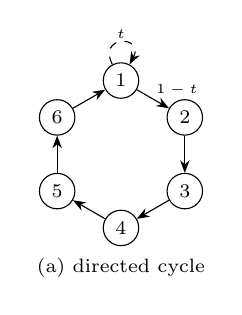
\begin{tikzpicture}[baseline=(c.base), scale=0.72]
        \foreach \i in {1,...,6} {
          \node[agent] (d\i) at ({90-60*(\i-1)}:1.3) {\i};
        }
        \node (c) at (0,0) {};
        \foreach \i/\j in {2/3,3/4,4/5,5/6,6/1} {
          \draw[edge] (d\i) -- (d\j);
        }
        \draw[edge] (d1) -- node[weight, above right] {$1-t$} (d2);
        % REVISED (2026-11-19, arrows: the dashed loop was narrow and hard to see). Was:
        % \draw[selfloop, dashed] (d1) to node[weight, above] {$t$} (d1);
        \draw[edge, dashed] (d1) to[out=118, in=62, looseness=5, min distance=4mm]
          node[weight, above] {$t$} (d1);
        \node at (0,-2.0) {\scriptsize (a) directed cycle};
      \end{tikzpicture}
      \hspace{1mm}
      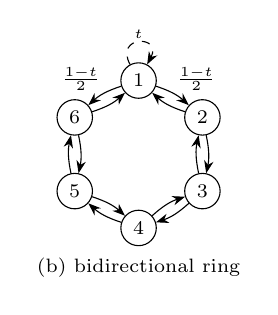
\begin{tikzpicture}[baseline=(c.base), scale=0.72]
        \foreach \i in {1,...,6} {
          \node[agent] (b\i) at ({90-60*(\i-1)}:1.3) {\i};
        }
        \node (c) at (0,0) {};
        \foreach \i/\j in {2/3,3/4,4/5,5/6} {
          \draw[edge] (b\i) to[bend left=12] (b\j);
          \draw[edge] (b\j) to[bend left=12] (b\i);
        }
        \draw[edge] (b2) to[bend left=12] (b1);
        \draw[edge] (b6) to[bend right=12] (b1);
        \draw[edge] (b1) to[bend left=12] node[weight, above right] {$\frac{1-t}{2}$} (b2);
        \draw[edge] (b1) to[bend right=12] node[weight, above left] {$\frac{1-t}{2}$} (b6);
        % REVISED (2026-11-19, arrows: the dashed loop was narrow and hard to see). Was:
        % \draw[selfloop, dashed] (b1) to node[weight, above] {$t$} (b1);
        \draw[edge, dashed] (b1) to[out=118, in=62, looseness=5, min distance=4mm]
          node[weight, above] {$t$} (b1);
        \node at (0,-2.0) {\scriptsize (b) bidirectional ring};
      \end{tikzpicture}

      \vspace{2mm}
      % REVISED (2026-11-19, notes of 19/11: the weights of the unlabelled edges; on the ring
      % agents 2 and 6 listen to agent 1 with weight 1/2 for every t). Was:
      % {\scriptsize Figure 1. Edge $i \to j$: agent $i$ is influenced by agent $j$\\
      % (course convention).}
      {\scriptsize Figure 1. Edge $i \to j$: agent $i$ is influenced by agent $j$ (course
      convention). Unlabelled edges: weight $1$ in (a), $1/2$ in (b).\par}

      % ADDED (2026-11-16, notes: the properties of the networks depend on t).
      % REVISED (2026-11-19, notes of 19/11: the cases of t come after the parametrization: the
      % table appears at the second step).
      \begin{uncoverenv}<2->
      \vspace{1mm}% REVISED (2026-11-19, layout). Was: \vspace{2mm}
      {\scriptsize
      \renewcommand{\arraystretch}{1.1}
      \begin{tabular}{@{}lccc@{}}
        \toprule
        Both networks & $t = 0$ & $0 < t < 1$ & $t = 1$ \\
        \midrule
        strongly connected & yes & yes & no \\
        aperiodic          & no  & yes & -- \\
        doubly-stochastic  & yes & no  & no \\
        \bottomrule
      \end{tabular}

      \smallskip
      --: not strongly connected, periodicity not defined (Definition~1.2).\par}
      \end{uncoverenv}
    % REVISED (2026-11-16, notes: the properties hold for t = 0 only, with the period of
    % each network; for t > 0 see the table under Figure 1). Was:
    % \column{0.52\textwidth}
    %   \small
    %   \begin{itemize}
    %     \item $n = 6$. Cycle: $a_{i,i+1} = 1$. Ring: $a_{i,i-1} = a_{i,i+1} = 1/2$
    %           (indices modulo $6$).
    %     \item Strongly connected and \alert{periodic} (period $6$ and $2$),
    %           doubly-stochastic: $\frac16\mathbf{1}_6$ is the left eigenvector associated
    %           with the eigenvalue $1$, no agent favoured.
    %     \item Only the row of agent~$1$ changes, $t \in [0,1]$:
    %           \[ a_1(t)^\top = (1-t)\, a_1^\top + t\, e_1^\top \;\to\; A(t), \]
    %           so $t = a_{11}$, the \alert{self-weight} of agent~$1$: from the original
    %           network ($t = 0$) to agent~$1$ stubborn ($t = 1$).
    %     \item $x(0) = (0,\, 0.2,\, 0.4,\, 0.6,\, 0.8,\, 1)^\top$, unless stated otherwise.
    %   \end{itemize}
    % REVISED (2026-11-11, terms: for t = 0 there is no consensus, so 1/6 1_6 is only the
    % left eigenvector of the eigenvalue 1, not a social power; indices modulo 6; x(0)
    % changes in Figures 7 and 12). Was:
    % \column{0.52\textwidth}
    %   \small
    %   \begin{itemize}
    %     \item $n = 6$. Cycle: $a_{i,i+1} = 1$. Ring: $a_{i,i\pm1} = 1/2$.
    %     \item Strongly connected and \alert{periodic} (period $6$ and $2$), doubly
    %           stochastic: $w = \frac16\mathbf{1}_6$, no agent favoured.
    %     \item Only agent~$1$ changes, with self-weight $t$:
    %           \[ a_1(t)^\top = (1-t)\, a_1^\top + t\, e_1^\top \;\to\; A(t), \]
    %           from the original network ($t = 0$) to agent~$1$ stubborn ($t = 1$).
    %     \item Always $x(0) = (0,\, 0.2,\, 0.4,\, 0.6,\, 0.8,\, 1)^\top$.
    %   \end{itemize}
    % REVISED (2026-11-19, notes of 19/11: first the networks and how they are parametrized,
    % then the case t = 0, which was described before t was defined; the parametrization
    % in words, with the row of agent 1 of each network). Was:
    % \column{0.52\textwidth}
    %   \small
    %   \begin{itemize}
    %     \item $n = 6$. Directed cycle: $a_{i,i+1} = 1$. Bidirectional ring:
    %           $a_{i,i-1} = a_{i,i+1} = 1/2$ (indices modulo $6$).
    %     \item For $t = 0$ both networks are strongly connected and \alert{periodic}, with
    %           period $6$ (directed cycle) and $2$ (bidirectional ring), and
    %           doubly-stochastic: in both, $\frac16\mathbf{1}_6$ is the left eigenvector
    %           associated with the eigenvalue $1$, and no agent is favoured.
    %     \item Only the row of agent~$1$ changes, $t \in [0,1]$:
    %           \[ a_1(t)^\top = (1-t)\, a_1^\top + t\, e_1^\top \;\to\; A(t), \]
    %           so $t = a_{11}$, the \alert{self-weight} of agent~$1$: from the original
    %           networks ($t = 0$) to agent~$1$ stubborn ($t = 1$).
    %     \item $x(0) = (0,\, 0.2,\, 0.4,\, 0.6,\, 0.8,\, 1)^\top$, unless stated otherwise.
    %   \end{itemize}
    % REVISED (2026-11-19, layout). Was: \column{0.52\textwidth}
    \column{0.54\textwidth}
      \footnotesize
      % REVISED (2026-11-21, layout: with the notation in full the column overflowed; the
      % setup on the first step, the case t = 0 on the second, with the rule recalled).
      \only<1>{%
      \begin{itemize}
        \setlength{\itemsep}{1pt}% ADDED (2026-11-19, layout)
        \item $n = 6$. Directed cycle: $a_{i,i+1} = 1$. Bidirectional ring:
              $a_{i,i-1} = a_{i,i+1} = 1/2$ (indices modulo $6$).
        % REVISED (2026-11-21, notes of 21/11: the notation of the rows said in full,
        % a_1(0) instead of a_1, e_1 defined, the original rows written out). Was:
        % \item Agent~$1$ gives weight $t \in [0,1]$ to itself and scales its original
        %       weights by $1 - t$: $a_1(t)^\top = (1-t)\, a_1^\top + t\, e_1^\top$, with
        %       $a_1^\top$ the row of agent~$1$ at $t = 0$. The other rows do not change;
        %       $A(t)$ is the resulting matrix.
        % \item Directed cycle: $a_1(t)^\top = (t,\, 1-t,\, 0,\, 0,\, 0,\, 0)$;
        %       bidirectional ring: $a_1(t)^\top = \bigl(t,\, \frac{1-t}{2},\, 0,\, 0,\, 0,\,
        %       \frac{1-t}{2}\bigr)$. So $t = a_{11}$, the \alert{self-weight} of agent~$1$:
        %       from the original networks ($t = 0$) to agent~$1$ stubborn ($t = 1$).
        \item Agent~$1$ gives weight $t \in [0,1]$ to itself and scales its original
              weights by $1 - t$, with the same rule on both networks:
              \[ a_1(t)^\top = (1-t)\, a_1(0)^\top + t\, e_1^\top, \]
              with $a_1(0)^\top$ the row of agent~$1$ in the original network and
              $e_1^\top = (1, 0, \dots, 0)$. The other rows do not change: $A(t)$ is the
              resulting matrix, $a_1(t)^\top$ its row of agent~$1$.
      \end{itemize}
      % REVISED (2026-11-21, notes of 21/11: the two rows in a small table).
      {\centering\scriptsize
      \renewcommand{\arraystretch}{1.25}
      \begin{tabular}{@{}lcc@{}}
        \toprule
        & $a_1(0)^\top$ & $a_1(t)^\top$ \\
        \midrule
        directed cycle & $(0, 1, 0, 0, 0, 0)$ & $(t,\, 1-t,\, 0,\, 0,\, 0,\, 0)$ \\
        bidirectional ring & $(0, \frac12, 0, 0, 0, \frac12)$
          & $\bigl(t,\, \frac{1-t}{2},\, 0,\, 0,\, 0,\, \frac{1-t}{2}\bigr)$ \\
        \bottomrule
      \end{tabular}\par}
      \begin{itemize}
        \setlength{\itemsep}{1pt}
        \item So $t = a_{11}$, the \alert{self-weight} of agent~$1$: from the original
              networks ($t = 0$) to agent~$1$ stubborn ($t = 1$).
        \item $x(0) = (0,\, 0.2,\, 0.4,\, 0.6,\, 0.8,\, 1)^\top$, unless stated otherwise.
      \end{itemize}}%
      \only<2>{%
      \begin{itemize}
        \item Row of agent~$1$: $a_1(t)^\top = (1-t)\, a_1(0)^\top + t\, e_1^\top$,
              $t \in [0,1]$, the same rule on both networks; the other rows as in the
              original networks.
        \item For $t = 0$ both networks are strongly connected and \alert{periodic}, with
              period $6$ (directed cycle) and $2$ (bidirectional ring), and
              doubly-stochastic: in both, $\frac16\mathbf{1}_6$ is the left eigenvector
              associated with the eigenvalue $1$, and no agent is favoured.
      \end{itemize}}
  \end{columns}
  \detailbuttons{\go{bk-graphs}{Graphs}}
\end{frame}

\begin{frame}[label=m-fdg-conv]{One self-weight brings agreement}
  \begin{columns}[T]
    \column{0.58\textwidth}
      \centering
      \includegraphics[width=\linewidth]{fdg_convergence.eps}

      % REVISED (2026-11-11, terms: the conditions of each case written in full; "on a
      % strongly connected network", as in the report). Was:
      % {\scriptsize Figure 2. Top: directed cycle; bottom: ring. Agent~$1$ dotted.}
      % \column{0.40\textwidth}
      %   \footnotesize
      %   \begin{itemize}
      %     \item $t = 0$: periodic, \alert{no convergence} (case ii).
      %     \item $0 < t < 1$: the self-loop makes $G$ aperiodic, $A(t)$ primitive
      %           (Corollary~1.12): \alert{consensus} (case i).
      %     \item $t = 1$: agent~$1$ stubborn, consensus on $x_1(0) = 0$ (case iii); in $5$
      %           steps on the cycle.
      %     \item Spectrum: for $t = 0$ eigenvalues $\neq 1$ on the unit circle, for $t > 0$
      %           strictly inside.
      %   \end{itemize}
      %   \vspace{1mm}
      %   \sociallycol{One agent that gives weight to its current opinion, without being stubborn,
      % is enough for the whole group to agree.}
      {\scriptsize Figure 2. Columns: $t = 0, \frac12, 1$. Top: directed cycle; bottom:
      bidirectional ring. Agent~$1$ marked with dots.}
    \column{0.40\textwidth}
      \footnotesize
      \begin{itemize}
        \item $t = 0$: periodic: \alert{no convergence} (case (ii)).
        \item $0 < t < 1$: strongly connected with a self-loop, $A(t)$ primitive
              (Corollary~1.12): \alert{consensus} (case (i)).
        \item $t = 1$: agent~$1$ stubborn, the only globally reachable node:
              \alert{consensus} on $x_1(0) = 0$ (case (iii)).
        % REVISED (2026-11-18, precision): the eigenvalue 1 stays on the unit circle. Was:
        % \item Spectrum: $t = 0$, some eigenvalues $\neq 1$ on the unit circle; $t > 0$,
        %       all strictly inside the unit disk.
        \item Spectrum: $t = 0$, some eigenvalues $\neq 1$ on the unit circle; $t > 0$,
              all eigenvalues $\neq 1$ strictly inside the unit disk.
      \end{itemize}
      \sociallycol{One agent that gives weight to its current opinion, without being
  stubborn, is enough, on a strongly connected network, for the whole group to agree.}
  \end{columns}
  \detailbuttons{\go{bk-spectra}{Spectra}}
\end{frame}

\begin{frame}[label=m-fdg-sp]{Social power grows gradually}
  \begin{columns}[T]
    \column{0.52\textwidth}
      \centering
      \includegraphics[width=\linewidth]{fdg_social_power.eps}

      % REVISED (2026-11-11, terms: w(t) is a social power only for t in (0,1], where
      % there is a consensus; w_1 -> 1/6 is a limit for t -> 0). Was:
      % {\scriptsize Figure 3. Dots: directed cycle; crosses: ring.}
      % \column{0.46\textwidth}
      %   \footnotesize
      %   \begin{itemize}
      %     \item On both networks
      %           \[ w(t) = \frac{(1,\ 1-t,\ \dots,\ 1-t)^\top}{1 + 5(1-t)}. \]
      %     \item $w_1$ grows from $1/6$ to $1$; at $t = \frac12$: $w_1 = \frac27$,
      %           $w_i = \frac17$.
      %     \item Consensus value $w(t)^\top x(0) = \dfrac{3(1-t)}{6-5t}$, i.e.\ $3/7$ at
      %           $t = \frac12$.
      %     \item The network decides \emph{how} the opinions converge, not \emph{where}.
      %   \end{itemize}
      {\scriptsize Figure 3. Top: $w_1$, $w_2$; bottom: consensus value. Dots: directed
      cycle; crosses: bidirectional ring.}
    \column{0.46\textwidth}
      \footnotesize
      \begin{itemize}
        \item For $t \in (0,1]$ (consensus), on both networks
              \[ w(t) = \frac{(1,\ 1-t,\ \dots,\ 1-t)^\top}{1 + 5(1-t)}. \]
        \item $w_1$ grows from $1/6$ ($t \to 0$) to $1$ ($t = 1$); at $t = \frac12$:
              $w_1 = \frac27$, $w_i = \frac17$ for $i \neq 1$.
        % REVISED (2026-11-21, notes of 21/11: the consensus value depends on x(0), w(t)
        % does not). Was:
        % \item Consensus value $w(t)^\top x(0) = \dfrac{3(1-t)}{6-5t}$, i.e.\ $3/7$ at
        %       $t = \frac12$.
        \item Consensus value, for $x(0) = (0,\, 0.2,\, \dots,\, 1)^\top$:
              $w(t)^\top x(0) = \dfrac{3(1-t)}{6-5t}$, i.e.\ $3/7$ at $t = \frac12$.
        \item Same values on both networks: the network decides \emph{how} the opinions
              converge, not \emph{where}.
      \end{itemize}
      \vspace{1mm}
      % REVISED (2026-11-16, terms: for t = 0 there is no consensus). Was:
      % \sociallycol{Inertia earns influence little by little: for $t < 1$ every initial opinion
      % still enters the consensus.}
      \sociallycol{Inertia earns influence little by little: for $0 < t < 1$ every initial
  opinion still enters the consensus.}
  \end{columns}
  \detailbuttons{\go{bk-socialpower}{Derivation}}
\end{frame}

% ADDED (2026-11-16, notes): why the two networks have the same social power, first the
% intuition and then the check of Section 2.2.3 of the report. Everything holds only for
% t in (0,1], where there is a consensus. The intuition is our reading of that check.
% REVISED (2026-11-17, preview): the column "Check (report, Section 2.2.3)" was
% misleading; the balance, said in full, is the whole argument (existence and, by
% uniqueness, the social power); the algebra stays in the backup "Derivation". Was:
% \begin{frame}[label=m-fdg-why]{Why the same social power}
%   \compactblocks
%   \footnotesize
%   For $t \in (0,1]$ the model reaches a consensus, and the social power solves
%   $w_j = \sum_{i} w_i\, a_{ij}(t)$ ($w^\top A(t) = w^\top$): each agent passes its social
%   power on to the agents it listens to, in proportion to the weights, and $w_j$ is what
%   agent~$j$ collects.
%   \begin{columns}[T]
%     \column{0.48\textwidth}
%       \begin{block}{Intuition}
%         \footnotesize
%         \begin{itemize}
%           \item $A(0)$ is doubly-stochastic: every agent is listened to with total weight
%                 $1$. The balance holds when every agent passes on the same amount.
%           \item Agents $2, \dots, 6$ have no self-loop and pass on all of their $b$;
%                 agent~$1$ keeps the share $t$ and passes on $(1-t)\,w_1$.
%           \item Hence $(1-t)\,w_1 = b$: agent~$1$ weighs $1/(1-t)$ times any other agent
%                 ($\frac27$ against $\frac17$ at $t = \frac12$).
%           \item Only \emph{how much} agent~$1$ keeps matters, not \emph{whom} it listens
%                 to: the same $w(t)$ on both networks.
%         \end{itemize}
%       \end{block}
%     \column{0.48\textwidth}
%       \begin{block}{Check (report, Section 2.2.3)}
%         \footnotesize
%         Substitute $w = (w_1, b, \dots, b)$ in $w^\top A(t) = w^\top$, with
%         $a_{1j}(t) = (1-t)\,a_{1j}(0)$ for $j \neq 1$, $a_{11}(0) = 0$, and the columns of
%         $A(0)$ summing to $1$:
%         \begin{itemize}
%           \item $j \neq 1$: $w_j = (1-t)\,w_1\,a_{1j}(0) + b\,\bigl(1 - a_{1j}(0)\bigr)$,
%                 which equals $b$ for every $j \neq 1$ iff $b = (1-t)\,w_1$;
%           \item $j = 1$: $w_1 = t\,w_1 + b$, again $b = (1-t)\,w_1$;
%           \item $w_1 + 5b = 1$ gives $w(t)$ of the previous slide; $t = 1$ gives
%                 $w = e_1$.
%           \item As $t \to 0$, $w(t) \to \frac16\mathbf{1}_6$. At $t = 0$ there is no
%                 consensus: $\frac16\mathbf{1}_6$ is only the left eigenvector of $A(0)$
%                 associated with the eigenvalue $1$.
%         \end{itemize}
%       \end{block}
%   \end{columns}
% \end{frame}
% TODO (2026-11-18, notes of Leonardo): to be redone and reworked. Kept for now, but it
% does not feel his own: the balance with b = "what every agent passes on" is not in the
% report, where b is the common social power of agents 2-6 (w = (w_1, b, ..., b)
% substituted in w^T A(t) = w^T, Section 2.2.3).
% REVISED (2026-11-18, notes of Leonardo): the balance reading ("each agent passes its
% social power on to the agents it listens to") replaced by the rule w_j = sum_i w_i a_ij
% (row j of w^T A = w^T) and the intuition agreed on 18/11: at t = 0 the columns of A(0)
% sum to 1, so the structure favours no agent; for t > 0 only the row of agent 1 changes,
% in the same way in both networks; then the check of the report (Section 2.2.3).
% DONE (2026-11-18): the TODO above is done. Was:
% \begin{frame}[label=m-fdg-why]{Why the same social power}
%   \compactblocks
%   \footnotesize
%   For $t \in (0,1]$ there is a consensus, and $w$ is the unique solution of
%   $w^\top A(t) = w^\top$ with $\mathbf{1}_6^\top w = 1$.
%   \begin{columns}[T]
%     \column{0.52\textwidth}
%       \begin{block}{$w^\top A(t) = w^\top$ read as a balance}
%         \footnotesize
%         \begin{itemize}
%           \item $w_j = \sum_i w_i\, a_{ij}(t)$: each agent passes its social power on to
%                 the agents it listens to, in proportion to the weights; $w_j$ is what
%                 agent~$j$ collects, its own share included.
%           \item In $A(0)$ every agent is listened to with total weight $1$
%                 (doubly-stochastic).
%           \item Changing $t$, agent~$1$ changes only how much it keeps; it passes on the
%                 rest with the weights of $A(0)$.
%           \item So, if every agent passes on the same amount $b$, every agent collects
%                 exactly $b$.
%         \end{itemize}
%       \end{block}
%     \column{0.44\textwidth}
%       \begin{block}{Hence}
%         \footnotesize
%         \begin{itemize}
%           \item Agents $2, \dots, 6$ keep nothing: $w_j = b$.
%           \item Agent~$1$ keeps $t\,w_1$: $w_1 = t\,w_1 + b$, i.e.\ $b = (1-t)\,w_1$.
%           \item With $w_1 + 5b = 1$: the $w(t)$ of the previous slide. The solution is
%                 unique, so it is the social power.
%           \item Agent~$1$ weighs $1/(1-t)$ times any other agent ($\frac27$ against
%                 $\frac17$ at $t = \frac12$).
%         \end{itemize}
%       \end{block}
%   \end{columns}
%   \begin{alertblock}{Only \emph{how much} agent~$1$ keeps matters, not \emph{whom} it listens to}
%     \footnotesize
%     The same $w(t)$ on both networks. As $t \to 0$, $w(t) \to \frac16\mathbf{1}_6$; at
%     $t = 0$ there is no consensus: $\frac16\mathbf{1}_6$ is only the left eigenvector of $A(0)$.
%   \end{alertblock}
% \end{frame}
% REVISED (2026-11-21, notes of 21/11: the slide repeated the computation of the report
% (the guess with b). Now a short chain that only recalls what the report contains: same
% social power = same limit of the powers (Theorem 2.2); what the two matrices have in
% common; hence the same w(t)). Was:
% \begin{frame}[label=m-fdg-why,t]{Why the same social power}
%   % [t]: the two steps start at the same height
%   \compactblocks
%   \footnotesize
%   \only<1>{%
%   \begin{columns}[T]
%     \column{0.47\textwidth}
%       \begin{block}{The rule behind $w$}
%         \footnotesize
%         $w^\top A = w^\top$, row $j$: \quad $w_j = \sum_i w_i\, a_{ij}$.
%
%         \smallskip
%         The weight of $x_j(0)$ in the consensus is the sum, over the agents $i$ that
%         listen to $j$ ($j$ itself included, if $a_{jj} > 0$), of the weight $a_{ij}$ with
%         which $i$ listens to $j$, times the weight $w_i$ of $x_i(0)$.
%       \end{block}
%     \column{0.51\textwidth}
%       \begin{block}{$t = 0$: the structure favours no agent}
%         \footnotesize
%         \begin{itemize}
%           \item In $A(0)$ every column sums to $1$ (doubly-stochastic): for every agent
%                 $j$, the weights with which the agents listen to $j$ sum to $1$. Directed
%                 cycle: $j$ is listened to only by agent $j-1$, with weight $1$. Ring: by
%                 agents $j-1$ and $j+1$, with weight $1/2$ each.
%           \item Hence equal weights satisfy the rule: $\frac16\mathbf{1}_6$ in both
%                 networks.
%           \item At $t = 0$ there is no consensus: $\frac16\mathbf{1}_6$ is not a social
%                 power, only the starting point (the limit of $w(t)$ as $t \to 0$).
%         \end{itemize}
%       \end{block}
%   \end{columns}
%
%   \medskip
%   For $t > 0$ only the row of agent~$1$ changes, in the same way in both networks:
%   weight $t$ on its own opinion, $1 - t$ on the opinions it listened to, in the same
%   proportions as before.}%
%   \only<2>{%
%   Suppose agents $2, \dots, 6$ all have the same weight $b$.\par
%   \vspace{-1.5mm}
%   \begin{columns}[T]
%     \column{0.41\textwidth}
%       \begin{block}{Agent~$1$}
%         \footnotesize
%         \begin{itemize}
%           \item The agents that listen to agent~$1$ are those of $t = 0$, with total
%                 weight $1$; in addition, agent~$1$ keeps weight $t$ on its own opinion.
%           \item Hence $w_1 = t\,w_1 + b$, so $w_1 > b$: the consensus value moves
%                 towards $x_1(0)$.
%         \end{itemize}
%       \end{block}
%     \column{0.57\textwidth}
%       \begin{block}{Agents $2, \dots, 6$}
%         \footnotesize
%         \begin{itemize}
%           \item Those that agent~$1$ does not listen to are listened to as at $t = 0$:
%                 they receive $b$.
%           \item Those that agent~$1$ listens to (cycle: $2$; ring: $2$ and $6$) receive
%                 from agent~$1$ the share $(1-t)\,a_{1j}\,w_1 = a_{1j}\,b$ ($a_{1j}$ as in
%                 $A(0)$), because $(1-t)\,w_1 = b$: the same share they received at
%                 $t = 0$ from an agent of weight $b$. They receive $b$ too.
%           \item The rule holds for every agent: the guess is consistent.
%         \end{itemize}
%       \end{block}
%   \end{columns}
%   \vspace{-2mm}
%   \begin{alertblock}{Hence the same $w(t)$ on both networks}
%     \footnotesize Only two facts are used: the columns of $A(0)$ sum to $1$, and the row
%     of agent~$1$ changes in the same way. How many agents listen to an agent, and in which
%     direction, does not enter: agent~$3$ receives $b \cdot 1$ on the cycle,
%     $b \cdot \frac12 + b \cdot \frac12$ on the ring. The network decides how the opinions
%     converge (Figure~2), not where.
%   \end{alertblock}
%   {\scriptsize Check (report, Section~2.2.3): substituting $w = (w_1, b, \dots, b)$ in
%   $w^\top A(t) = w^\top$, all the equations reduce to $b = (1-t)\,w_1$; with
%   $w_1 + 5b = 1$, the $w(t)$ of the previous slide, unique for $t > 0$ (eigenvalue $1$
%   simple).\par}}
% \end{frame}
% REVISED (2026-11-23, notes of 23/11: one slide instead of three steps). Was:
% \begin{frame}[label=m-fdg-why,t]{Why the same social power}
%   % REVISED (2026-11-21, notes of 21/11: a sequential chain, in two steps: the fact and
%   % the question; then what the limit depends on, the same starting point, the same
%   % change, hence the same limit).
%   \compactblocks
%   \small
%   \only<1>{%
%   \begin{block}{The fact}
%     \small
%     Same social power on the two networks $\iff$ same limit of the powers: by (A2) of
%     Theorem~2.2, for $t \in (0,1]$,
%     \[ \lim_{k \to \infty} A(t)^k = \mathbf{1}_6\, w(t)^\top . \]
%     No $x(0)$ here: $w(t)$ depends only on $A(t)$, and $x(0)$ enters only the consensus
%     value $w(t)^\top x(0)$.
%   \end{block}
%   \begin{block}{The puzzle}
%     \small
%     The two matrices $A(t)$ are different: on the directed cycle every agent listens to one
%     agent, on the bidirectional ring to two. Their spectra are different too.
%   \end{block}
%   \medskip
%   \alert{What do they have in common that gives the same limit?}}%
%   \only<2>{%
%   \begin{block}{Step by step}
%     \small
%     \begin{enumerate}
%       \item \textbf{What the limit depends on.} For $t > 0$ the eigenvalue $1$ is simple
%             and the others lie strictly inside the unit disk, so by Theorem~2.2 the limit is
%             $\mathbf{1}_6\, w(t)^\top$, with $w(t)^\top A(t) = w(t)^\top$. The other
%             eigenvalues do not enter: same limit $\iff$ same $w(t)$.
%       \item \textbf{The same starting point.} At $t = 0$ both matrices are
%             doubly-stochastic: every agent is listened to with total weight $1$, and
%             $w = \frac16\mathbf{1}_6$: all agents count the same.
%       \item \textbf{The same change.} For $t > 0$ only the row of agent~$1$ changes, with
%             the same rule on both networks: agent~$1$ keeps $t$ for itself and listens to
%             the others with $1 - t$ times its old weights.
%     \end{enumerate}
%   \end{block}}%
%   \only<3>{%
%   \begin{block}{Step by step}
%     \small
%     \begin{enumerate}
%       \setcounter{enumi}{3}
%       \item \textbf{The equation for $w(t)$.} Column $j$ of $w(t)^\top A(t) = w(t)^\top$
%             reads $w_j = \sum_i w_i\, a_{ij}(t)$. Suppose agents $2, \dots, 6$ have the
%             same social power $b$, as at $t = 0$.
%             \begin{itemize}
%               \item Column $1$: agent~$1$ listens to itself with weight $t$, and the others
%                     listen to it with total weight $1$, as at $t = 0$. So
%                     $w_1 = t\, w_1 + b$, i.e.\ $b = (1-t)\, w_1$.
%               \item Column $j \neq 1$: agent~$1$ listens to $j$ with weight
%                     $(1-t)\, a_{1j}(0)$; multiplied by $w_1 = b/(1-t)$, this gives
%                     $b\, a_{1j}(0)$, the same term as at $t = 0$, when agent~$1$ had the
%                     same social power $b$ as the others. So every column $j \neq 1$ is as at
%                     $t = 0$ and gives $w_j = b$: the supposition holds, on both networks,
%                     whether agent~$1$ listens to one agent or to two.
%             \end{itemize}
%       \item \textbf{Hence the same $w(t)$} $\propto (1,\, 1-t,\, \dots,\, 1-t)$ on both
%             networks, unique because the eigenvalue $1$ is simple: the same limit
%             $\mathbf{1}_6\, w(t)^\top$, the same social power. What differs between the two
%             networks decides how the opinions converge, not where.
%     \end{enumerate}
%   \end{block}}
% \end{frame}
\begin{frame}[label=m-fdg-why]{Why the same social power}
  \small
  Same social power on the two networks $\iff$ same limit of the powers: by (A2) of
  Theorem~2.2, for $t \in (0,1]$, $\lim_{k \to \infty} A(t)^k = \mathbf{1}_6\, w(t)^\top$,
  with $w(t)^\top A(t) = w(t)^\top$; no $x(0)$ here. Yet the two matrices are different:
  on the directed cycle every agent listens to one agent, on the bidirectional ring to two.

  \medskip
  \begin{enumerate}
    \setlength{\itemsep}{4pt}
    \item \textbf{The same starting point.} At $t = 0$ both matrices are doubly-stochastic:
          every agent is listened to with total weight $1$, and $w = \frac16\mathbf{1}_6$.
    \item \textbf{The same change.} For $t > 0$ only the row of agent~$1$ changes, with the
          same rule on both networks.
    \item \textbf{Hence the same $w(t)$.} Column $j$ of $w(t)^\top A(t) = w(t)^\top$ reads
          $w_j = \sum_i w_i\, a_{ij}(t)$. With agents $2, \dots, 6$ at the same $b$, as at
          $t = 0$: column~$1$ gives $w_1 = t\, w_1 + b$, i.e.\ $b = (1-t)\, w_1$; in every
          column $j \neq 1$ the term of agent~$1$ is $(1-t)\, a_{1j}(0)\, w_1 = b\,
          a_{1j}(0)$, as at $t = 0$, so $w_j = b$. Then
          $w(t) \propto (1,\, 1-t,\, \dots,\, 1-t)$ on both networks, unique because the
          eigenvalue $1$ is simple.
  \end{enumerate}

  \medskip
  \alert{What differs between the two networks decides how the opinions converge, not
  where.}
\end{frame}

% REVISED (2026-11-16, notes): the bridge is now in two steps (overlays), with the
% ring of Figure 1. Was:
% % ADDED (2026-11-16, order): bridge between the two models. Why no FDG example shows a
% % disagreement (a choice, as in the Introduction of the report), Remark 2.7, and the
% % idea of the FJ model.
% \begin{frame}[label=m-bridge]{From stubborn agents to prejudices}
%   \compactblocks
%   \begin{alertblock}{What the FDG examples show}
%     \footnotesize
%     In every FDG example $C(G)$ has a single sink: the whole network when $G$ is strongly
%     connected ($t < 1$), agent~$1$ when it is stubborn ($t = 1$). Hence no convergence or
%     consensus, cases (i)--(iii), and \emph{never} a disagreement, which needs $n_s \geq 2$
%     sinks (Theorem~2.4). This is a choice: the two models are compared on the same small
%     networks and with the same resisting agent, agent~$1$, so that every difference comes
%     from the model and not from the data.
%   \end{alertblock}
%   \begin{block}{Remark 2.7 (More than one stubborn agent)}
%     \footnotesize
%     If two or more agents are stubborn, each of them is a sink of $C(G)$ made of a single,
%     aperiodic node. If every other agent is influenced, directly or through
%     intermediaries, by at least one stubborn agent, these are the only sinks, and the
%     group converges (Corollary~2.6) to a disagreement (Theorem~2.4): every stubborn agent
%     keeps its own initial opinion, and every other agent converges to a convex
%     combination of the opinions of the stubborn agents it is influenced by (see
%     also [5]). Since there is no single consensus value, the social power is no longer
%     defined.
%   \end{block}
%   \small
%   \begin{minipage}{0.76\textwidth}
%     Several agents anchored to different fixed opinions: the starting point of the
%     \alert{FJ model}, in which every agent can resist \emph{partially}.
%   \end{minipage}
%   \detailbuttons{\go{bk-stubborn}{Stubborn agents}}
% \end{frame}

% REVISED (2026-11-16, notes): the bridge drew the stubborn opinions as inputs, which
% the FDG model does not have; it is now the single slide "Two stubborn agents" with
% the open question, and the second rewriting is the answer on m-back-question. Was:
% % ADDED (2026-11-16, notes): the bridge in two steps, on the bidirectional ring.
% % Step 1: two stubborn agents, two aperiodic sinks, disagreement, no social power, and why
% % the FDG part does not simulate it (reasons 1 and 2). Step 2: the two stubborn agents
% % removed from the group become fixed opinions of the agents that listened to them (the
% % second rewriting of the report, Figure 8, here with two stubborn agents), then the FJ
% % model. Reason 3 is on the slide m-six-sinks.
% \begin{frame}[label=m-bridge]{From stubborn agents to prejudices}
%   \begin{columns}[T]
%     \column{0.40\textwidth}
%       \centering
%       \only<1>{%
%       \begin{tikzpicture}[scale=0.85]
%         \foreach \i in {1,...,6} {
%           \node[agent] (r\i) at ({90-60*(\i-1)}:1.3) {\i};
%         }
%         \node[agent, fill=red_unipd!15] at (r1) {1};
%         \node[agent, fill=red_unipd!15] at (r4) {4};
%         \draw[edge] (r2) to[bend left=12] (r3);
%         \draw[edge] (r3) to[bend left=12] (r2);
%         \draw[edge] (r5) to[bend left=12] (r6);
%         \draw[edge] (r6) to[bend left=12] (r5);
%         \draw[edge] (r2) -- (r1);
%         \draw[edge] (r6) -- (r1);
%         \draw[edge] (r3) -- (r4);
%         \draw[edge] (r5) -- (r4);
%         \draw[selfloop] (r1) to node[weight, above] {$1$} (r1);
%         \draw[edge] (r4) to[out=-115, in=-65, looseness=6, min distance=4mm]
%           node[weight, below] {$1$} (r4);
%       \end{tikzpicture}
%
%       {\scriptsize Bidirectional ring with agents $1$ and $4$ stubborn; unlabelled edges
%       have weight $1/2$.}}%
%       \only<2>{%
%       \begin{tikzpicture}[scale=0.85]
%         \foreach \i in {2,3,5,6} {
%           \node[agent] (s\i) at ({90-60*(\i-1)}:1.3) {\i};
%         }
%         \node[font=\scriptsize] (f1) at (90:1.3) {$x_1(0)$};
%         \node[font=\scriptsize] (f4) at (-90:1.3) {$x_4(0)$};
%         \draw[edge] (s2) to[bend left=12] (s3);
%         \draw[edge] (s3) to[bend left=12] (s2);
%         \draw[edge] (s5) to[bend left=12] (s6);
%         \draw[edge] (s6) to[bend left=12] (s5);
%         \draw[edge] (f1) -- (s2);
%         \draw[edge] (f1) -- (s6);
%         \draw[edge] (f4) -- (s3);
%         \draw[edge] (f4) -- (s5);
%       \end{tikzpicture}
%
%       {\scriptsize Agents $1$ and $4$ removed: their opinions enter agents $2, 6$ and
%       $3, 5$ as fixed values. Every arrow has weight $1/2$.}}
%     \column{0.58\textwidth}
%       \footnotesize
%       \only<1>{%
%       \textbf{Two stubborn agents}
%       \begin{itemize}
%         % REVISED (2026-11-16, notes: link with Figure 2). Was:
%         % \item $a_{11} = a_{44} = 1$: $C(G)$ has two sinks, $\{1\}$ and $\{4\}$, both
%         %       aperiodic because of their self-loops.
%         \item As in Figure~2 with $t = 1$, agent~$1$ is stubborn; now agent~$4$, opposite
%               to it, is stubborn too: $a_{11} = a_{44} = 1$.
%         \item $C(G)$ has two sinks, $\{1\}$ and $\{4\}$, both aperiodic because of their
%               self-loops.
%         \item Theorem~2.4: \alert{disagreement}. Agents $1$ and $4$ keep their opinions;
%               agents $2, 3, 5, 6$ converge to convex combinations of $x_1(0)$ and
%               $x_4(0)$ (Remark~2.7).
%         \item The rows of $\lim_{k \to \infty} A^k$ differ: no single vector plays the
%               role of $w$, and \alert{the social power is not defined}.
%       \end{itemize}
%       \smallskip
%       Not simulated in the FDG part, by choice: (1)~the FDG model is already covered in
%       the course, so its part is kept short; (2)~the social power, the answer to our
%       third question, requires a consensus. The disagreement will appear again in the FJ
%       part.}%
%       \only<2>{%
%       \textbf{Out of the group: fixed opinions}
%       \begin{itemize}
%         % REVISED (2026-11-16, notes: link with Figure 8 of the report). Was:
%         % \item A stubborn agent never changes its opinion: remove it, and its opinion
%         %       becomes a \alert{fixed opinion} of the agents that listened to it.
%         \item A stubborn agent never changes its opinion: remove it, and its opinion
%               becomes a \alert{fixed opinion} of the agents that listened to it, as in
%               Figure~8 of the report (there with agent~$1$ only).
%         \item Agent~$2$ now updates as $x_2(k+1) = \frac12\, x_3(k) + \frac12\, x_1(0)$,
%               and agents $3, 5, 6$ likewise: the same trajectories as before.
%         \item A fixed opinion of an agent is its \alert{prejudice}; the weight it gives to
%               it is its \alert{attachment}, here $1/2$.
%       \end{itemize}
%       \smallskip
%       Remark~2.7 is the starting point of the \alert{FJ model}: every agent may be anchored
%       to a prejudice of its own, with an attachment between $0$ and $1$, so that it can
%       resist the others \emph{partially}.}
%   \end{columns}
%   \detailbuttons{\go{bk-stubborn}{Stubborn agents}\ \go{bk-rewritings2}{Figure 8}}
% \end{frame}

% ADDED (2026-11-16, notes): end of the FDG part. Two stubborn agents on the ring: G and
% C(G) with the same layout, Theorem 2.4, no social power, why we stop here, and the
% question, first on this network and then in general. No inputs, no prejudices, no FJ
% model: the answer comes in the FJ part, on the slide m-back-question.
\begin{frame}[label=m-bridge]{Two stubborn agents}
  \begin{columns}[T]
    \column{0.42\textwidth}
      \centering
      % REVISED (2026-11-18, arrows): scale 0.52 -> 0.62, loop labels on the right and
      % captions higher, so that the slide keeps its height. Was:
      % \begin{tikzpicture}[scale=0.52]
      \begin{tikzpicture}[scale=0.62]
        % (a) G: bidirectional ring with agents 1 and 4 stubborn
        \foreach \i in {1,...,6} {
          \node[agent] (r\i) at ({90-60*(\i-1)}:1.3) {\i};
        }
        \node[agent, fill=red_unipd!15] at (r1) {1};
        \node[agent, fill=red_unipd!15] at (r4) {4};
        \draw[edge] (r2) to[bend left=12] (r3);
        \draw[edge] (r3) to[bend left=12] (r2);
        \draw[edge] (r5) to[bend left=12] (r6);
        \draw[edge] (r6) to[bend left=12] (r5);
        \draw[edge] (r2) -- (r1);
        \draw[edge] (r6) -- (r1);
        \draw[edge] (r3) -- (r4);
        \draw[edge] (r5) -- (r4);
        % REVISED (2026-11-18, arrows): loop labels on the right. Was:
        % \draw[selfloop] (r1) to node[weight, above] {$1$} (r1);
        % \draw[edge] (r4) to[out=-115, in=-65, looseness=6, min distance=4mm]
        %   node[weight, below] {$1$} (r4);
        % \node at (0,-3.05) {\scriptsize (a) $G$};
        \draw[selfloop] (r1) to node[weight, right] {$1$} (r1);
        \draw[edge] (r4) to[out=-115, in=-65, looseness=6, min distance=4mm]
          node[weight, right] {$1$} (r4);
        \node at (0,-2.75) {\scriptsize (a) $G$};
        % (b) C(G), same layout
        \begin{scope}[shift={(4.9,0)}]
          \node[agent, fill=red_unipd!15] (c1) at (90:1.3) {1};
          \node[agent, fill=red_unipd!15] (c4) at (-90:1.3) {4};
          \node[draw, rounded corners=2pt, font=\scriptsize, inner sep=2pt] (c23)
            at (0:1.4) {$\{2,3\}$};
          \node[draw, rounded corners=2pt, font=\scriptsize, inner sep=2pt] (c56)
            at (180:1.4) {$\{5,6\}$};
          \draw[edge] (c23) -- (c1);
          \draw[edge] (c23) -- (c4);
          \draw[edge] (c56) -- (c1);
          \draw[edge] (c56) -- (c4);
          % REVISED (2026-11-18, arrows): same height as (a). Was:
          % \node at (0,-3.05) {\scriptsize (b) $C(G)$: two sinks};
          \node at (0,-2.75) {\scriptsize (b) $C(G)$: two sinks};
        \end{scope}
      \end{tikzpicture}

      {\scriptsize Unlabelled edges of $G$: weight $1/2$.}
    \column{0.56\textwidth}
      \footnotesize
      \begin{itemize}
        \item As in Figure~2 with $t = 1$, agent~$1$ is stubborn; now also agent~$4$,
              opposite to it: $a_{11} = a_{44} = 1$.
        \item $C(G)$: two sinks, $\{1\}$ and $\{4\}$, aperiodic (self-loops).
              Theorem~2.4: \alert{disagreement}; $2, 3, 5, 6$ converge to convex
              combinations of $x_1(0)$ and $x_4(0)$ (Remark~2.7).
        \item Rows of $\lim_{k \to \infty} A^k$ differ: \alert{the social power is not
              defined}.
        \item We stop here: (1)~the FDG model is seen in the course; (2)~the social power
              requires a consensus.
      \end{itemize}
  \end{columns}
  \begin{minipage}{0.84\textwidth}
    \begin{alertblock}{A question we will come back to}
      \small
      Agents $1$ and $4$ never change their opinions: are they members of the group, or
      fixed opinions from outside that the others listen to?

      \smallskip
      In general: if an agent's opinion remains unchanged independent of the others'
      opinions, is it a member of the group, or a fixed opinion from outside that the
      others listen to?
    \end{alertblock}
  \end{minipage}
  \detailbuttons{\go{bk-stubborn}{Stubborn agents}}
\end{frame}

% ===========================================================================
\section{The Friedkin--Johnsen model}
% ===========================================================================

% REVISED (2026-11-11, terms: equation numbers; names of W, lambda_i and u as in the
% report; lambda_i = 0 gives x_i(k) = u_i for k >= 1, stubborn only if u_i = x_i(0);
% original FJ assumptions). Was:
% \begin{frame}[label=m-fj-model]{The FJ model}
%   \[ x(k+1) = \Lambda W x(k) + (I - \Lambda)\, u, \qquad
%      x_i(k+1) = \lambda_i \textstyle\sum_{j} w_{ij}\, x_j(k) + (1-\lambda_i)\, u_i \]
%   \begin{columns}[T]
%     \column{0.5\textwidth}
%       \small
%       \begin{itemize}
%         \item $W$: row-stochastic, social influences (the role of $A$).
%         \item $\Lambda = \operatorname{diag}(\lambda_i)$, $\lambda_i \in [0,1]$:
%               susceptibility.
%         \item $u$: constant \alert{prejudices}; $1 - \lambda_i$: \alert{attachment} of
%               agent $i$ to $u_i$.
%       \end{itemize}
%     \column{0.48\textwidth}
%       \small
%       \begin{itemize}
%         \item $\lambda_i = 1$: FDG rule ($\Lambda = I$ excluded).
%         \item $\lambda_i < 1$: agent $i$ \alert{prejudiced}.
%         \item $\lambda_i = 0$, $u_i = x_i(0)$: agent $i$ \alert{stubborn}.
%       \end{itemize}
%   \end{columns}
\begin{frame}[label=m-fj-model]{The FJ model}
  \[ x(k+1) = \Lambda W x(k) + (I - \Lambda)\, u \;\; (4), \qquad
     x_i(k+1) = \lambda_i \textstyle\sum_{j} w_{ij}\, x_j(k) + (1-\lambda_i)\, u_i
     \;\; (5) \]
  \begin{columns}[T]
    \column{0.5\textwidth}
      \footnotesize
      \begin{itemize}
        \item $W$: row-stochastic, the \emph{matrix of social influences}, weighted
              adjacency matrix of $G$ (the role of $A$).
        \item $\Lambda = \operatorname{diag}(\lambda_1, \dots, \lambda_n)$,
              $\lambda_i \in [0,1]$: \emph{susceptibility} of agent $i$ to social
              influence.
        % REVISED (2026-11-16, notes: what a prejudice is, in words). Was:
        % \item $u$: constant vector of the agents' \alert{prejudices}; $1 - \lambda_i$:
        %       \alert{attachment} of agent $i$ to its prejudice.
        \item $u$: constant vector of the agents' \alert{prejudices}, fixed opinions that
              the agents listen to; $1 - \lambda_i$: \alert{attachment} of agent $i$ to its
              prejudice.
      \end{itemize}
    \column{0.48\textwidth}
      \footnotesize
      \begin{itemize}
        \item $\lambda_i = 1$: agent $i$ follows the FDG rule. $\Lambda = I$ is the FDG
              model with $A = W$, so $\Lambda \neq I$ from now on.
        \item $\lambda_i < 1$: agent $i$ \alert{prejudiced}.
        \item $\lambda_i = 0$: $x_i(k) = u_i$ for all $k \geq 1$; \alert{stubborn}
              (Definition~2.5) only if, in addition, $u_i = x_i(0)$.
        \item Original FJ model: $u = x(0)$ and $1 - \lambda_i = w_{ii}$. As in [5], not
              imposed here.
      \end{itemize}
  \end{columns}
  \vspace{3mm}
  \socially{A self-weight ties an agent to its \emph{current} opinion, which still moves
  towards the others; a prejudice ties it to a \emph{fixed} opinion, which never moves.}
\end{frame}

% REVISED (2026-11-11, terms): "P-dependent agents: always asymptotically stable" was
% wrong, since asymptotic stability is a property of a system: Theorem 3.2 states it for
% the subsystem (6). The definitions of convergence and asymptotic stability of the FJ
% model, Definition 3.1, Theorem 3.2 and Corollary 3.3 are now as in the report; the
% intuition with the error (10) stays in the backup slide bk-fj-stab, and the backup
% slide bk-fj-thm, which repeated Definition 3.1 and Theorem 3.2, is removed. Was:
% \begin{frame}[label=m-fj-conv]{Convergence in the FJ model}
%   \small
%   \textbf{P-dependent} (Definition~3.1 [5]): prejudiced, or influenced through a walk by a
%   prejudiced agent: \emph{a prejudice reaches it}.
%   \begin{block}{Theorem 3.2 [5], in words}
%     \footnotesize
%     P-dependent agents: always asymptotically stable, $\rho(\Lambda^{11}W^{11}) < 1$. The
%     model converges iff all agents are P-dependent or the P-independent ones (an FDG model
%     with $W^{22}$) converge, i.e.\ $W^{22}$ regular. Final opinions: convex combinations of
%     the prejudices and of the final opinions of the P-independent agents.
%   \end{block}
%   \begin{block}{Corollary 3.3 [5], in words}
%     \footnotesize
%     Asymptotically stable iff all agents are P-dependent (e.g.\ $\Lambda \neq I$ and $G$
%     strongly connected); then $x(\infty) = Vu$, $V = (I - \Lambda W)^{-1}(I - \Lambda)$.
%   \end{block}
%   \textbf{Intuition:} $e(k+1) = \Lambda W e(k)$; deviations leave only through prejudiced
%   agents. \alert{No aperiodicity needed.}
%   \detailbuttons{\go{bk-fj-thm}{Theorem 3.2}\ \go{bk-fj-stab}{Stability}}
% \end{frame}
% REVISED (2026-11-17, preview): split in two frames, m-fj-conv (all agents
% P-dependent, with the intuition written on the slide) and m-fj-conv2 (the general
% case, Theorem 3.2, with the meaning of W22 written on the slide). Was:
% \begin{frame}[label=m-fj-conv]{Convergence in the FJ model}
%   \compactblocks
%   \scriptsize
%   The FJ model (4) \emph{converges} if the limit $x(\infty) = \lim_{k \to +\infty} x(k)$
%   exists for every initial condition $x(0)$, and it is \emph{asymptotically stable} if
%   $\Lambda W$ is convergent, i.e.\ $\rho(\Lambda W) < 1$ (Definition~1.7,
%   Theorem~1.8) [5].
%   \begin{columns}[T]
%     \column{0.40\textwidth}
%       \begin{block}{Definition 3.1 (P-dependent agents) [5]}
%         Agent $i$ is \emph{P-dependent} if it is prejudiced or influenced by some
%         prejudiced agent $j$, that is, a walk from $i$ to $j$ in the graph $G$ exists.
%         Otherwise, the agent is \emph{P-independent}.
%       \end{block}
%       Agents $1, \dots, r$ P-dependent ($r \geq 1$, since $\Lambda \neq I$), agents
%       $r+1, \dots, n$ P-independent: $W^{21} = 0$, $\Lambda^{22} = I$, and [5]
%       \[ \begin{aligned}
%            x^1(k+1) &= \Lambda^{11}\bigl[W^{11} x^1(k) + W^{12} x^2(k)\bigr]\\
%                     &\quad + (I - \Lambda^{11})\, u^1, \hspace{2em} (6)\\
%            x^2(k+1) &= W^{22} x^2(k). \hspace{2em} (7)
%          \end{aligned} \]
%       (7): an FDG model, which no prejudice reaches.
%
%       \smallskip
%       \alert{No aperiodicity is needed} when all agents are P-dependent.
%     \column{0.58\textwidth}
%       \begin{block}{Theorem 3.2 [5]}
%         Let the community have $r \geq 1$ P-dependent agents and $n - r \geq 0$
%         P-independent ones. Then, the subsystem (6) is asymptotically stable, i.e.\
%         $\Lambda^{11} W^{11}$ is Schur stable $\rho(\Lambda^{11} W^{11}) < 1$. The model
%         (4) is convergent if and only if $r = n$ or (7) is convergent, i.e.\ $W^{22}$ is
%         regular. In this case
%         \[ x^1(\infty) = V \begin{bmatrix} u^1 \\ x^2(\infty) \end{bmatrix}, \;
%            V \triangleq (I_r - \Lambda^{11} W^{11})^{-1}
%            \begin{bmatrix} I_r - \Lambda^{11} & \Lambda^{11} W^{12} \end{bmatrix}.
%            \; (8) \]
%         The matrix $V$ is stochastic, i.e.\ the final opinion of any agent is a convex
%         combination of the prejudices and final opinions of P-independent agents.
%       \end{block}
%       \begin{block}{Corollary 3.3 [5]}
%         The Friedkin--Johnsen model (4) is asymptotically stable if and only if all
%         agents are P-dependent. Then, $V = (I - \Lambda W)^{-1}(I - \Lambda)$. This holds,
%         in particular, if $\Lambda < I_n$ or $\Lambda \neq I_n$ and $G$ is strongly
%         connected ($W$ is irreducible).
%       \end{block}
%   \end{columns}
%   \detailbuttons{\go{bk-fj-stab}{Stability}\ \go{bk-fj-stab2}{Spectrum}}
% \end{frame}
% REVISED (2026-11-19, notes of 19/11: order of the report, Section 3.1.2. Corollary 3.3
% gave V before Theorem 3.2 defines it, and the intuition used the V of the corollary.
% Now: definitions, P-dependent agents and the decomposition (6)-(7) here; Theorem 3.2 on
% m-fj-conv2; Corollary 3.3 as the case r = n, with the intuition, on m-fj-conv3).
% Was:
% \begin{frame}[label=m-fj-conv]{Convergence in the FJ model}
%   \compactblocks
%   \small
%   The FJ model (4) \emph{converges} if the limit $x(\infty) = \lim_{k \to +\infty} x(k)$
%   exists for every initial condition $x(0)$, and it is \emph{asymptotically stable} if
%   $\Lambda W$ is convergent, i.e.\ $\rho(\Lambda W) < 1$ (Definition~1.7,
%   Theorem~1.8) [5].
%   \begin{columns}[T]
%     \column{0.48\textwidth}
%       \begin{block}{Definition 3.1 (P-dependent agents) [5]}
%         \footnotesize
%         Agent $i$ is \emph{P-dependent} if it is prejudiced or influenced by some
%         prejudiced agent $j$, that is, a walk from $i$ to $j$ in the graph $G$ exists.
%         Otherwise, the agent is \emph{P-independent}.
%       \end{block}
%     \column{0.48\textwidth}
%       \begin{block}{Corollary 3.3 [5]}
%         \footnotesize
%         The Friedkin--Johnsen model (4) is asymptotically stable if and only if all
%         agents are P-dependent. Then, $V = (I - \Lambda W)^{-1}(I - \Lambda)$. This holds,
%         in particular, if $\Lambda < I_n$ or $\Lambda \neq I_n$ and $G$ is strongly
%         connected ($W$ is irreducible).
%       \end{block}
%   \end{columns}
%   \begin{alertblock}{Intuition}
%     \footnotesize
%     The deviation from the equilibrium, $e(k) = x(k) - Vu$, obeys
%     $e(k+1) = \Lambda W\, e(k)$: $u$ does not appear. $\Lambda W$ decides whether the
%     opinions converge, $u$ decides where. A prejudiced agent keeps only a fraction
%     $\lambda_i$ of the deviations it listens to: they die out only if every agent is
%     influenced by a prejudiced agent. \alert{No aperiodicity is needed.}
%   \end{alertblock}
%   \detailbuttons{\go{bk-fj-stab}{Stability}}
% \end{frame}
\begin{frame}[label=m-fj-conv]{Convergence in the FJ model}
  \compactblocks
  \small
  The FJ model (4) \emph{converges} if the limit $x(\infty) = \lim_{k \to +\infty} x(k)$
  exists for every initial condition $x(0)$, and it is \emph{asymptotically stable} if
  $\Lambda W$ is convergent, i.e.\ $\rho(\Lambda W) < 1$ (Definition~1.7,
  Theorem~1.8) [5].
  \begin{block}{Definition 3.1 (P-dependent agents) [5]}
    \footnotesize
    Agent $i$ is \emph{P-dependent} if it is prejudiced or influenced by some
    prejudiced agent $j$, that is, a walk from $i$ to $j$ in the graph $G$ exists.
    Otherwise, the agent is \emph{P-independent}.
  \end{block}
  \footnotesize
  A P-independent agent is not prejudiced ($\lambda_i = 1$) and is not influenced by any
  P-dependent agent. Since $\Lambda \neq I$, at least one agent is P-dependent. Numbering
  the P-dependent agents $1, \dots, r$ ($r \geq 1$) and the P-independent ones
  $r+1, \dots, n$, and splitting $x$, $u$, $W$, $\Lambda$ accordingly: $W^{21} = 0$,
  $\Lambda^{22} = I$, and [5]
  \begin{align*}
    x^1(k+1) &= \Lambda^{11}\bigl[W^{11} x^1(k) + W^{12} x^2(k)\bigr]
                + (I - \Lambda^{11})\, u^1, \tag{6}\\
    x^2(k+1) &= W^{22} x^2(k). \tag{7}
  \end{align*}
  $W^{22}$ says how the P-independent agents listen to each other; it is row-stochastic,
  since $W$ is row-stochastic and $W^{21} = 0$. Hence (7) is an FDG model among the
  P-independent agents, which no prejudice reaches; the P-dependent agents receive the
  opinions of the P-independent ones as an additional input.
\end{frame}

% ADDED (2026-11-17, preview): second half of the old frame m-fj-conv, the general case
% with P-independent agents (Theorem 3.2), with the meaning of W22 written on the slide.
% REVISED (2026-11-19, notes of 19/11: Theorem 3.2 alone, after the decomposition (6)-(7)
% of m-fj-conv; the box says where aperiodicity enters, as in the report). Was:
% \begin{frame}[label=m-fj-conv2]{Convergence with P-independent agents}
%   \compactblocks
%   \small
%   \begin{columns}[T]
%     \column{0.40\textwidth}
%       Agents $1, \dots, r$ P-dependent ($r \geq 1$, since $\Lambda \neq I$), agents
%       $r+1, \dots, n$ P-independent: $W^{21} = 0$, $\Lambda^{22} = I$, and [5]
%       \[ \begin{aligned}
%            x^1(k+1) &= \Lambda^{11}\bigl[W^{11} x^1(k) + W^{12} x^2(k)\bigr]\\
%                     &\quad + (I - \Lambda^{11})\, u^1, \hspace{2em} (6)\\
%            x^2(k+1) &= W^{22} x^2(k). \hspace{2em} (7)
%          \end{aligned} \]
%       $W^{22}$: how the P-independent agents listen to each other. (7) is an FDG model,
%       which no prejudice reaches.
%     \column{0.58\textwidth}
%       \begin{block}{Theorem 3.2 [5]}
%         \scriptsize
%         Let the community have $r \geq 1$ P-dependent agents and $n - r \geq 0$
%         P-independent ones. Then, the subsystem (6) is asymptotically stable, i.e.\
%         $\Lambda^{11} W^{11}$ is Schur stable $\rho(\Lambda^{11} W^{11}) < 1$. The model
%         (4) is convergent if and only if $r = n$ or (7) is convergent, i.e.\ $W^{22}$ is
%         regular. In this case
%         \[ x^1(\infty) = V \begin{bmatrix} u^1 \\ x^2(\infty) \end{bmatrix}, \;
%            V \triangleq (I_r - \Lambda^{11} W^{11})^{-1}
%            \begin{bmatrix} I_r - \Lambda^{11} & \Lambda^{11} W^{12} \end{bmatrix}.
%            \; (8) \]
%         The matrix $V$ is stochastic, i.e.\ the final opinion of any agent is a convex
%         combination of the prejudices and final opinions of P-independent agents.
%       \end{block}
%   \end{columns}
%   \begin{alertblock}{Aperiodicity is needed again, but only for the P-independent agents}
%     \footnotesize
%     The FJ model converges if and only if all agents are P-dependent, or the FDG model (7)
%     of the P-independent agents converges.
%   \end{alertblock}
%   \detailbuttons{\go{bk-fj-stab2}{Spectrum}}
% \end{frame}
\begin{frame}[label=m-fj-conv2]{Convergence with P-independent agents}
  \compactblocks
  \begin{block}{Theorem 3.2 [5]}
    \footnotesize
    Let the community have $r \geq 1$ P-dependent agents and $n - r \geq 0$
    P-independent ones. Then, the subsystem (6) is asymptotically stable, i.e.\
    $\Lambda^{11} W^{11}$ is Schur stable $\rho(\Lambda^{11} W^{11}) < 1$. The model
    (4) is convergent if and only if $r = n$ or (7) is convergent, i.e.\ $W^{22}$ is
    regular. In this case
    \[ x^1(\infty) = V \begin{bmatrix} u^1 \\ x^2(\infty) \end{bmatrix}, \qquad
       V \triangleq (I_r - \Lambda^{11} W^{11})^{-1}
       \begin{bmatrix} I_r - \Lambda^{11} & \Lambda^{11} W^{12} \end{bmatrix}.
       \qquad (8) \]
    The matrix $V$ is stochastic, i.e.\ the final opinion of any agent is a convex
    combination of the prejudices and final opinions of P-independent agents.
  \end{block}
  \begin{alertblock}{Aperiodicity is needed again, but only for the P-independent agents}
    \footnotesize
    The FJ model converges if and only if all agents are P-dependent, or the FDG model (7)
    of the P-independent agents converges. By the Rosetta stone, (7) converges if and only
    if all the sinks of the condensation digraph of the subgraph of the P-independent
    agents are aperiodic.
  \end{alertblock}
  \detailbuttons{\go{bk-fj-stab2}{Spectrum}}
\end{frame}

% ADDED (2026-11-19, notes of 19/11): Corollary 3.3 as the case r = n of Theorem 3.2, with the
% intuition of the report (equation (10)); before, on m-fj-conv, ahead of Theorem 3.2.
\begin{frame}[label=m-fj-conv3]{All agents P-dependent}
  \compactblocks
  \small
  Here $r = n$ in Theorem~3.2: no P-independent agents, and the subsystem (6) is the whole
  model.
  \begin{block}{Corollary 3.3 [5]}
    \footnotesize
    The Friedkin--Johnsen model (4) is asymptotically stable if and only if all
    agents are P-dependent. Then, $V = (I - \Lambda W)^{-1}(I - \Lambda)$. This holds,
    in particular, if $\Lambda < I_n$ or $\Lambda \neq I_n$ and $G$ is strongly
    connected ($W$ is irreducible).
  \end{block}
  % ADDED (2026-11-22, notes of 21/11): why all agents must be P-dependent; shown later.
  {\footnotesize With P-independent agents the model may still converge, but it is not
  asymptotically stable: the limit depends on their initial opinions, as we will see in
  «Where no prejudice arrives».\par}
  With $r = n$, (8) gives, for every $x(0)$, \ $x(\infty) = Vu$ \ (9), with $V$ as in
  Corollary~3.3.
  % REVISED (2026-11-23, notes of 23/11: a shorter intuition). Was:
  % \begin{alertblock}{Intuition}
  %   \footnotesize
  %   $Vu$ is an equilibrium of (4), since $(I - \Lambda W)V = I - \Lambda$. The deviation
  %   $e(k) = x(k) - Vu$ obeys $e(k+1) = \Lambda W\, e(k)$ (10): $u$ does not appear.
  %   $\Lambda W$ decides whether the opinions converge, $u$ decides where. At each step
  %   agent $i$ keeps a fraction $\lambda_i$ of the weighted average of the deviations it
  %   listens to: the deviations leave the group only through the prejudiced agents, and
  %   vanish only if every agent is influenced, directly or through intermediaries, by one
  %   of them. \alert{No aperiodicity is needed}, unlike in the FDG model.
  % \end{alertblock}
  \begin{alertblock}{Intuition}
    \footnotesize
    $Vu$ is the equilibrium of (4), since $(I - \Lambda W)V = I - \Lambda$. The deviation
    $e(k) = x(k) - Vu$ obeys $e(k+1) = \Lambda W\, e(k)$ (10), where $u$ does not appear.
    The model is asymptotically stable, so $e(k) \to 0$ for every $x(0)$.
  \end{alertblock}
  \detailbuttons{\go{bk-fj-stab}{Stability}}
\end{frame}

\begin{frame}[label=m-fj-final]{Final opinions and the augmented graph}
  \begin{columns}[T]
    % REVISED (2026-11-11, terms): in the FJ model consensus is defined for a given u
    % and characterized only when all agents are P-dependent; case (iv) of the augmented
    % model holds when all its sinks are aperiodic, and with all agents P-dependent the
    % only sinks are the virtual agents. Was:
    % \column{0.56\textwidth}
    %   \small
    %   All P-dependent: $x_i(\infty) = \sum_j v_{ij}\, u_j$.
    %   \begin{itemize}
    %     \item The initial opinions are \alert{forgotten}.
    %     \item Only prejudices of prejudiced agents count.
    %     \item \alert{Consensus iff all prejudiced agents share the same prejudice}.
    %   \end{itemize}
    %   \textbf{Augmented graph [5].} A prejudice is a virtual stubborn agent $i'$:
    %   \[ \bar A = \begin{bmatrix} \Lambda W & I - \Lambda \\ 0 & I \end{bmatrix} \]
    %   FDG model on $2n$ agents; virtual agents are aperiodic sinks: case (iv).
    \column{0.56\textwidth}
      \footnotesize
      All agents P-dependent: $x(\infty) = Vu$ (9), i.e.\
      $x_i(\infty) = \sum_{j} v_{ij}\, u_j$:
      \begin{itemize}
        % REVISED (2026-11-23, notes of 23/11). Was:
        % \item the initial opinions are \alert{forgotten}: $x(0)$ does not appear in
        %       $x(\infty)$;
        \item $x(0)$ does not appear in $x(\infty)$;
        \item only the prejudices of prejudiced agents count ($\lambda_j = 1$: column $j$
              of $V$ is zero);
        \item for a given $u$, \alert{consensus} ($x(\infty) = \gamma\,\mathbf{1}_n$) iff
              all the prejudiced agents have the same prejudice.
      \end{itemize}
      % REVISED (2026-11-16, notes: link to the bridge, read backwards). Was:
      % \textbf{Augmented model [5].} Agent $i$ gets a virtual stubborn agent $i'$,
      % $x_{i'}(k) = u_i$ for all $k$:
      % REVISED (2026-11-16, notes: the new bridge has no inputs). Was:
      % \textbf{Augmented model [5]}, the bridge read backwards: agent $i$ gets a virtual
      % stubborn agent $i'$, with $x_{i'}(k) = u_i$ for all $k$:
      \textbf{Augmented model [5].} Agent $i$ gets a virtual stubborn agent $i'$, with
      $x_{i'}(k) = u_i$ for all $k$:
      \[ \bar A = \begin{bmatrix} \Lambda W & I - \Lambda \\ 0 & I \end{bmatrix}
         \quad (11), \]
      % REVISED (2026-11-16, order: link back to the disagreement of Theorem 2.4). Was:
      % row-stochastic: an FDG model on $2n$ agents. Each virtual agent is an aperiodic
      % sink; with all agents P-dependent they are the only sinks: \alert{case (iv)}, with
      % limit (9).
      % REVISED (2026-11-19, notes of 19/11: the disagreement of the augmented model, which the
      % example of Figure 4 does not show, is discussed on m-back-question). Was:
      % row-stochastic: an FDG model on $2n$ agents. Each virtual agent is an aperiodic
      % sink; with all agents P-dependent they are the only sinks: \alert{case (iv)}, the
      % disagreement of Theorem~2.4, with limit (9).
      row-stochastic: an FDG model on $2n$ agents. Each virtual agent is stubborn: a sink
      of the augmented graph, aperiodic because of its self-loop.
    \column{0.42\textwidth}
      \centering
      % REVISED (2026-11-18, arrows): scale 0.55 -> 0.63. Was:
      % \begin{tikzpicture}[baseline=(c.base), scale=0.55]
      \begin{tikzpicture}[baseline=(c.base), scale=0.63]
        \foreach \i in {1,...,6} {
          \node[agent] (p\i) at ({90-60*(\i-1)}:1.3) {\i};
        }
        \node (c) at (0,0) {};
        \foreach \i/\j in {2/3,3/4,4/5,5/6,6/1} {
          \draw[edge] (p\i) -- (p\j);
        }
        \draw[edge] (p1) -- node[weight, above right] {$\lambda_1$} (p2);
        % REVISED (2026-11-18, arrows): u_1 lower, so that the slide keeps its height. Was:
        % \draw[edge] (0,2.7) node[above, font=\scriptsize] {$u_1$}
        \draw[edge] (0,2.45) node[above, font=\scriptsize] {$u_1$}
          -- node[weight, right] {$1-\lambda_1$} (p1);
        \node at (0,-2.0) {\scriptsize (a) FJ model};
      \end{tikzpicture}
      % REVISED (2026-11-18, arrows): scale 0.55 -> 0.63. Was:
      % \begin{tikzpicture}[baseline=(c.base), scale=0.55]
      \begin{tikzpicture}[baseline=(c.base), scale=0.63]
        \foreach \i in {1,...,6} {
          \node[agent] (a\i) at ({90-60*(\i-1)}:1.3) {\i};
        }
        \node (c) at (0,0) {};
        \foreach \i/\j in {2/3,3/4,4/5,5/6,6/1} {
          \draw[edge] (a\i) -- (a\j);
        }
        \draw[edge] (a1) -- node[weight, above right] {$\lambda_1$} (a2);
        % REVISED (2026-11-18, arrows): 1' lower, as u_1. Was:
        % \node[agent, dashed, minimum size=5.5mm] (v1) at (0,2.7) {$1'$};
        \node[agent, dashed, minimum size=5.5mm] (v1) at (0,2.45) {$1'$};
        \draw[edge] (a1) -- node[weight, right] {$1-\lambda_1$} (v1);
        \draw[selfloop] (v1) to node[weight, above] {$1$} (v1);
        \node at (0,-2.0) {\scriptsize (b) augmented graph};
      \end{tikzpicture}

      {\scriptsize Figure 4. Agent~$1$ the only prejudiced agent.}

      % REVISED (2026-11-18, arrows): no extra space, the buttons stay below the block.
      % Was: \vspace{1mm}
      \raggedright
      % REVISED (2026-11-11, layout: green block in the right column). Was:
      % \socially{A prejudice behaves as an extra agent that never changes its opinion,
      % placed beside the prejudiced agent.}
      \sociallycol{A prejudice behaves as an extra agent that never changes its opinion,
      placed beside the prejudiced agent.}
  \end{columns}
  \detailbuttons{\go{bk-fj-consensus}{Consensus}\ \go{bk-augmented}{Augmented}}
\end{frame}

% MOVED (2026-11-18, order): from after m-back-question (notes of 18/11). The theory part
% ends with the definition; the answer to the question then leads straight to the
% examples.
\begin{frame}[label=m-fj-centrality]{Influence centrality}
  \compactblocks
  \small
  \begin{itemize}
    % REVISED (2026-11-23, notes of 23/11: the sentence on the sinks removed; as in the
    % report, Section 3.1.3). Was:
    % \item The social power requires a consensus, which in the FJ model is not a property
    %       of the model but depends on $u$; the augmented model has at least $n$ sinks, so
    %       for $n \geq 2$ it never reaches a consensus.
    \item The social power requires a consensus for every $x(0)$. In the FJ model
          $x(\infty) = Vu$ does not depend on $x(0)$, and whether the final opinions
          coincide depends on $u$.
    \item As in [5]: asymptotically stable FJ model with $u = x(0)$, the traditional
          assumption of the FJ theory. It gives the initial opinions a role:
          $x(\infty) = V x(0)$.
  \end{itemize}
  \begin{block}{Influence centrality [5]}
    \[ c = n^{-1} V^\top \mathbf{1}_n, \qquad
       \bar x = \frac{1}{n} \sum_{i=1}^{n} x_i(\infty) = c^\top x(0) \qquad (12) \]
    \footnotesize $c_i$, the \emph{influence centrality} of agent $i$: the mean weight of its
    initial opinion in determining the group members' final opinions, i.e.\ the mean of
    column $i$ of $V$. $V$ is stochastic, so $c \geq 0$ and $c^\top\mathbf{1}_n = 1$, like $w$.
  \end{block}
\end{frame}

% REVISED (2026-11-17, preview): moved here from after m-state-input; the
% question is repeated on the slide; the answer starts from the augmented model read
% backwards; "a member of the group" no longer refers to the slide m-state-input,
% which now comes later. Was:
% \begin{frame}[label=m-back-question]{Back to the question}
%   \begin{columns}[T]
%     \column{0.46\textwidth}
%       \centering
%       \begin{tikzpicture}[scale=0.55]
%         % (a) the FDG model of the slide m-bridge
%         \foreach \i in {1,...,6} {
%           \node[agent] (q\i) at ({90-60*(\i-1)}:1.3) {\i};
%         }
%         \node[agent, fill=red_unipd!15] at (q1) {1};
%         \node[agent, fill=red_unipd!15] at (q4) {4};
%         \draw[edge] (q2) to[bend left=12] (q3);
%         \draw[edge] (q3) to[bend left=12] (q2);
%         \draw[edge] (q5) to[bend left=12] (q6);
%         \draw[edge] (q6) to[bend left=12] (q5);
%         \draw[edge] (q2) -- (q1);
%         \draw[edge] (q6) -- (q1);
%         \draw[edge] (q3) -- (q4);
%         \draw[edge] (q5) -- (q4);
%         \draw[selfloop] (q1) to node[weight, above] {$1$} (q1);
%         \draw[edge] (q4) to[out=-115, in=-65, looseness=6, min distance=4mm]
%           node[weight, below] {$1$} (q4);
%         \node at (0,-3.05) {\scriptsize (a) FDG model};
%         % (b) the FJ model on agents 2, 3, 5, 6 (second rewriting)
%         \begin{scope}[shift={(4.9,0)}]
%           \foreach \i in {2,3,5,6} {
%             \node[agent] (s\i) at ({90-60*(\i-1)}:1.3) {\i};
%           }
%           \node[font=\scriptsize] (f1) at (90:1.5) {$x_1(0)$};
%           \node[font=\scriptsize] (f4) at (-90:1.5) {$x_4(0)$};
%           \draw[edge] (s2) to[bend left=12] (s3);
%           \draw[edge] (s3) to[bend left=12] (s2);
%           \draw[edge] (s5) to[bend left=12] (s6);
%           \draw[edge] (s6) to[bend left=12] (s5);
%           \draw[edge] (f1) -- (s2);
%           \draw[edge] (f1) -- (s6);
%           \draw[edge] (f4) -- (s3);
%           \draw[edge] (f4) -- (s5);
%           \node at (0,-3.05) {\scriptsize (b) FJ model};
%         \end{scope}
%       \end{tikzpicture}
%
%       {\scriptsize (b) Agents $1$ and $4$ removed: their opinions enter as prejudices,
%       with weight $1 - \lambda_i = 1/2$. As in Figure~4(a), the edges carry the weights
%       of $\Lambda W$: $\lambda_2 w_{23} = 1/2$, since $w_{23} = 1$. Every arrow has
%       weight $1/2$.}
%     \column{0.52\textwidth}
%       \footnotesize
%       Second rewriting of the report (Figure~8, there with agent~$1$ only): remove the
%       stubborn agents; their opinions become the prejudices of the agents that listened
%       to them,
%       \[ x_2(k+1) = \tfrac12\, x_3(k) + \tfrac12\, x_1(0): \quad
%          \lambda_2 = \tfrac12,\ u_2 = x_1(0), \]
%       and likewise $u_6 = x_1(0)$, $u_3 = u_5 = x_4(0)$, all with $\lambda_i = 1/2$:
%       the same trajectories.
%       \begin{alertblock}{Answer: both readings hold}
%         \footnotesize
%         \emph{A member of the group}: the rewriting of [5] of the previous slide,
%         $\lambda_i = 0$, $u_i = x_i(0)$.\\
%         \emph{A fixed opinion from outside}: a prejudice of the agents that listen to it,
%         as here.\\
%         Both give the same trajectories. The disagreement of the two stubborn agents is
%         the disagreement of agents anchored to different prejudices.
%       \end{alertblock}
%   \end{columns}
%   \detailbuttons{\go{bk-rewritings2}{Figure 8}}
% \end{frame}
\begin{frame}[label=m-back-question,t]{Back to the question}
  % [t]: the figure and the question do not move between the two steps
  \compactblocks
  \begin{alertblock}{The question of the slide «Two stubborn agents»}
    \footnotesize
    Agents $1$ and $4$ never change their opinions: are they members of the group, or
    fixed opinions from outside that the others listen to?
  \end{alertblock}
  \begin{columns}[T]
    \column{0.46\textwidth}
      \centering
      % REVISED (2026-11-17, arrows): scale 0.44 -> 0.66; at 0.44 the agents almost touched and
      % the arrows had no room. Was:
      % \begin{tikzpicture}[scale=0.44]
      \begin{tikzpicture}[scale=0.66]
        % (a) the FDG model of the slide m-bridge
        \foreach \i in {1,...,6} {
          \node[agent] (q\i) at ({90-60*(\i-1)}:1.3) {\i};
        }
        \node[agent, fill=red_unipd!15] at (q1) {1};
        \node[agent, fill=red_unipd!15] at (q4) {4};
        \draw[edge] (q2) to[bend left=12] (q3);
        \draw[edge] (q3) to[bend left=12] (q2);
        \draw[edge] (q5) to[bend left=12] (q6);
        \draw[edge] (q6) to[bend left=12] (q5);
        \draw[edge] (q2) -- (q1);
        \draw[edge] (q6) -- (q1);
        \draw[edge] (q3) -- (q4);
        \draw[edge] (q5) -- (q4);
        \draw[selfloop] (q1) to node[weight, above] {$1$} (q1);
        \draw[edge] (q4) to[out=-115, in=-65, looseness=6, min distance=4mm]
          node[weight, below] {$1$} (q4);
        % REVISED (2026-11-17, arrows): label closer to the graph. Was:
        % \node at (0,-3.05) {\scriptsize (a) FDG model};
        \node at (0,-2.75) {\scriptsize (a) FDG model};
        % (b) the FJ model on agents 2, 3, 5, 6 (second rewriting)
        % REVISED (2026-11-17, arrows): shift 4.9 -> 4.6. Was:
        % \begin{scope}[shift={(4.9,0)}]
        \begin{scope}[shift={(4.6,0)}]
          \foreach \i in {2,3,5,6} {
            \node[agent] (s\i) at ({90-60*(\i-1)}:1.3) {\i};
          }
          % REVISED (2026-11-17, arrows): the prejudices further from agents 2, 3, 5, 6. Was:
          % \node[font=\scriptsize] (f1) at (90:1.5) {$x_1(0)$};
          % \node[font=\scriptsize] (f4) at (-90:1.5) {$x_4(0)$};
          \node[font=\scriptsize] (f1) at (90:1.85) {$x_1(0)$};
          \node[font=\scriptsize] (f4) at (-90:1.85) {$x_4(0)$};
          \draw[edge] (s2) to[bend left=12] (s3);
          \draw[edge] (s3) to[bend left=12] (s2);
          \draw[edge] (s5) to[bend left=12] (s6);
          \draw[edge] (s6) to[bend left=12] (s5);
          \draw[edge] (f1) -- (s2);
          \draw[edge] (f1) -- (s6);
          \draw[edge] (f4) -- (s3);
          \draw[edge] (f4) -- (s5);
          % REVISED (2026-11-17, arrows): same height as (a). Was:
          % \node at (0,-3.05) {\scriptsize (b) FJ model};
          \node at (0,-2.75) {\scriptsize (b) FJ model};
        \end{scope}
      \end{tikzpicture}

      {\scriptsize (b) Every arrow has weight $1/2$: the prejudices $1 - \lambda_i$, the
      edges $\lambda_2 w_{23}$ ($w_{23} = 1$), as in Figure~4(a).}
    \column{0.52\textwidth}
      \footnotesize
      \only<1>{%
      The augmented model reads a prejudice as a virtual stubborn agent; read backwards,
      a stubborn agent is a prejudice of the agents that listen to it. Removing $1$ and
      $4$ (report, Figure~8, there with agent~$1$ only):
      \[ x_2(k+1) = \tfrac12\, x_3(k) + \tfrac12\, x_1(0): \ \lambda_2 = \tfrac12,\
         u_2 = x_1(0); \]
      likewise $u_6 = x_1(0)$, $u_3 = u_5 = x_4(0)$, all with $\lambda_i = \tfrac12$:
      the same trajectories.}%
      \only<2>{%
      \begin{alertblock}{Answer: both readings hold}
        \footnotesize
        \emph{A member of the group}: an FJ agent with $\lambda_i = 0$, $u_i = x_i(0)$,
        i.e.\ stubborn, the others with $\lambda_i = 1$.

        \smallskip
        \emph{A fixed opinion from outside}: a prejudice of the agents that listen to it,
        as here.

        \smallskip
        Both give the same trajectories: the disagreement of the two stubborn agents is
        the disagreement of agents anchored to different prejudices.
      \end{alertblock}}
  \end{columns}
  \detailbuttons{\go{bk-rewritings2}{Figure 8}}
\end{frame}

% REVISED (2026-11-11, terms): why the social power cannot be used, as in the report;
% the influence centrality and Lemma 3.5 as in the report; what "fully regular" means.
% Was:
% \begin{frame}[label=m-fj-centrality]{Influence centrality}
%   \small
%   \begin{itemize}
%     \item The social power needs a consensus: in the FJ model it depends on $u$, and the
%           augmented graph has $\geq n$ sinks.
%     \item As in [5]: asymptotically stable, $u = x(0)$ (traditional FJ), so
%           $x(\infty) = V x(0)$.
%   \end{itemize}
%   \begin{block}{Influence centrality [5]}
%     \[ c = n^{-1} V^\top \mathbf{1}_n, \qquad
%        \bar x = \tfrac1n \textstyle\sum_{i} x_i(\infty) = c^\top x(0) \]
%     \footnotesize $c_i$: mean weight of $x_i(0)$ in the final opinions;
%     $c \geq 0$, $c^\top\mathbf{1}_n = 1$, like $w$.
%   \end{block}
%   \begin{block}{Lemma 3.5 [5], in words}
%     \footnotesize With $\Lambda = \alpha I$ and $W$ fully regular, $c_\alpha \to w$ as
%     $\alpha \to 1^-$; for $\alpha = 0$, $V = I$ and $c_0 = \frac1n\mathbf{1}_n$.
%   \end{block}
%   \detailbuttons{\go{bk-centrality}{Lemma 3.5}}
% \end{frame}
% REVISED (2026-11-17, preview): only the definition; the case alpha = 0 and Lemma 3.5
% moved to the slide m-lemma, where they are used. Was:
% \begin{frame}[label=m-fj-centrality]{Influence centrality}
%   \compactblocks
%   \footnotesize
%   \begin{itemize}
%     \item The social power requires a consensus, which in the FJ model is not a property
%           of the model but depends on $u$; the augmented model has at least $n$ sinks, so
%           for $n \geq 2$ it never reaches a consensus.
%     \item As in [5]: asymptotically stable FJ model with $u = x(0)$, the traditional
%           assumption of the FJ theory; then $x(\infty) = V x(0)$.
%   \end{itemize}
%   \begin{block}{Influence centrality [5]}
%     \[ c = n^{-1} V^\top \mathbf{1}_n, \qquad
%        \bar x = \frac{1}{n} \sum_{i=1}^{n} x_i(\infty) = c^\top x(0) \qquad (12) \]
%     \scriptsize $c_i$, the \emph{influence centrality} of agent $i$: the mean weight of its
%     initial opinion in determining the group members' final opinions. $V$ is stochastic,
%     so $c \geq 0$ and $c^\top\mathbf{1}_n = 1$, like $w$.
%   \end{block}
%   With $\Lambda = \alpha I_n$, $\alpha \in [0,1)$: $V_\alpha$ and $c_\alpha$; for
%   $\alpha = 0$, $V = I$ and $c_0 = n^{-1}\mathbf{1}_n$ [5].
%   \begin{block}{Lemma 3.5 [5]}
%     \scriptsize Let $W$ be a fully regular matrix and $w$ stand for the vector of French's
%     social power, corresponding to the FDG model (1) with $A = W$. Then,
%     $w = \lim_{\alpha \to 1-0} c_\alpha$.
%   \end{block}
%   \begin{minipage}{0.76\textwidth}
%     \scriptsize $W$ \alert{fully regular} (Definition~1.9):
%     $\lim_{k \to \infty} W^k = \mathbf{1}_n w^\top$, i.e.\ the FDG model with $A = W$
%     reaches a consensus [5].
%   \end{minipage}
%   \detailbuttons{\go{bk-centrality}{Lemma 3.5}}
% \end{frame}
% MOVED (2026-11-18, order): the active frame m-fj-centrality is now right after
% m-fj-final, before m-back-question (notes of 18/11).

% ADDED (2026-11-18, notes of 18/11): the networks of the examples drawn, before the
% table. The FJ networks are built by analogy with the FDG ones: same edges and weights,
% the self-weight becomes the weight of a prejudice. Not a rewriting of one model as the
% other, except for t = 1 in (a)-(b), the rewriting of [5]. (d) is the network whose
% augmented graph is drawn in m-six-sinks, with the same layout.
% REVISED (2026-11-19, notes of 19/11: the bidirectional ring has its own slide,
% m-fj-graphs-ring; the two titles say which network, on one line). Was:
% \begin{frame}[label=m-fj-graphs]{The networks of the examples}
\begin{frame}[label=m-fj-graphs]{Example networks: directed cycle}
  \noindent
  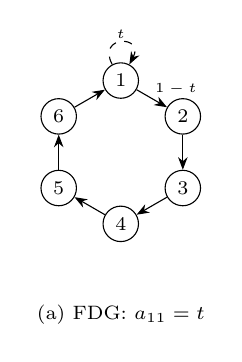
\begin{tikzpicture}[baseline=(c.base), scale=0.7]
    \foreach \i in {1,...,6} {
      \node[agent] (na\i) at ({90-60*(\i-1)}:1.3) {\i};
    }
    \node (c) at (0,0) {};
    \foreach \i/\j in {2/3,3/4,4/5,5/6,6/1} {
      \draw[edge] (na\i) -- (na\j);
    }
    \draw[edge] (na1) -- node[weight, above right] {$1-t$} (na2);
    % REVISED (2026-11-19, arrows: the dashed loop was narrow and hard to see). Was:
    % \draw[selfloop, dashed] (na1) to node[weight, right] {$t$} (na1);
    \draw[edge, dashed] (na1) to[out=118, in=62, looseness=5, min distance=4mm]
      node[weight, above] {$t$} (na1);
    \node at (0,-2.95) {\scriptsize (a) FDG: $a_{11} = t$};
  \end{tikzpicture}\hfill
  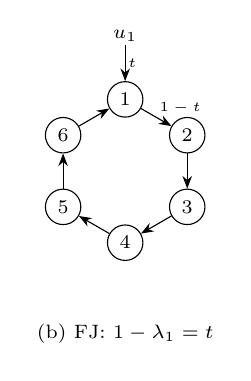
\begin{tikzpicture}[baseline=(c.base), scale=0.7]
    \foreach \i in {1,...,6} {
      \node[agent] (nb\i) at ({90-60*(\i-1)}:1.3) {\i};
    }
    \node (c) at (0,0) {};
    \foreach \i/\j in {2/3,3/4,4/5,5/6,6/1} {
      \draw[edge] (nb\i) -- (nb\j);
    }
    \draw[edge] (nb1) -- node[weight, above right] {$1-t$} (nb2);
    \node[font=\scriptsize, inner sep=1pt] (ub1) at (90:2.45) {$u_1$};
    \draw[edge] (ub1) -- node[weight, right] {$t$} (nb1);
    \node at (0,-2.95) {\scriptsize (b) FJ: $1 - \lambda_1 = t$};
  \end{tikzpicture}\hfill
  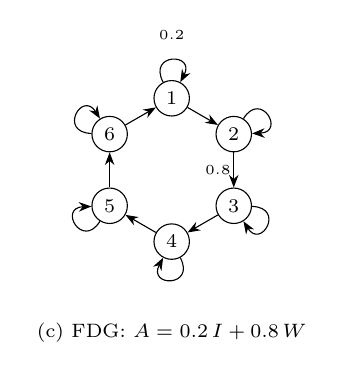
\begin{tikzpicture}[baseline=(c.base), scale=0.7]
    \foreach \i in {1,...,6} {
      \pgfmathsetmacro{\ang}{90-60*(\i-1)}
      \pgfmathsetmacro{\angout}{\ang+28}
      \pgfmathsetmacro{\angin}{\ang-28}
      \node[agent] (nc\i) at (\ang:1.3) {\i};
      \draw[edge] (nc\i) to[out=\angout, in=\angin, looseness=5, min distance=4mm] (nc\i);
    }
    \node (c) at (0,0) {};
    \foreach \i/\j in {1/2,3/4,4/5,5/6,6/1} {
      \draw[edge] (nc\i) -- (nc\j);
    }
    \draw[edge] (nc2) -- node[weight, left] {$0.8$} (nc3);
    \node[weight] at (90:2.45) {$0.2$};
    \node at (0,-2.95) {\scriptsize (c) FDG: $A = 0.2\,I + 0.8\,W$};
  \end{tikzpicture}\hfill
  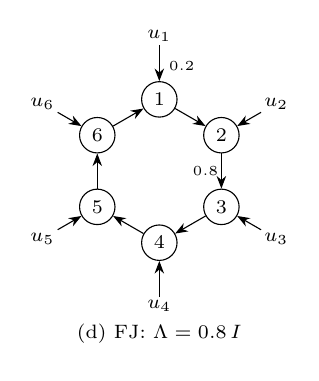
\begin{tikzpicture}[baseline=(c.base), scale=0.7]
    \foreach \i in {1,...,6} {
      \pgfmathsetmacro{\ang}{90-60*(\i-1)}
      \node[agent] (nd\i) at (\ang:1.3) {\i};
      \node[font=\scriptsize, inner sep=1pt] (ud\i) at (\ang:2.45) {$u_{\i}$};
      \draw[edge] (ud\i) -- (nd\i);
    }
    \node (c) at (0,0) {};
    \foreach \i/\j in {1/2,3/4,4/5,5/6,6/1} {
      \draw[edge] (nd\i) -- (nd\j);
    }
    \draw[edge] (nd2) -- node[weight, left] {$0.8$} (nd3);
    \node[weight] at (78:1.95) {$0.2$};
    \node at (0,-2.95) {\scriptsize (d) FJ: $\Lambda = 0.8\,I$};
  \end{tikzpicture}

  \smallskip
  % REVISED (2026-11-19, notes of 19/11: the ring is drawn on the next slide). Was:
  % {\scriptsize Directed cycle of Figure~1(a); the bidirectional ring in the same way. FJ
  % model: $W = A(0)$, $u = x(0)$. Unlabelled edges: weight $1$ in (a), (b) and $0.8$ in
  % (c), (d), where every self-loop and every prejudice has weight $0.2$.\par}
  % REVISED (2026-11-22, notes of 22/11: the FJ panels draw the weights of Lambda W, as in
  % the report (Figures 5, 8, 11); the caption said only W = A(0)). Was:
  % {\scriptsize Directed cycle of Figure~1(a). FJ model: $W = A(0)$, $u = x(0)$. Unlabelled
  % edges: weight $1$ in (a), (b) and $0.8$ in (c), (d), where every self-loop and every
  % prejudice has weight $0.2$.\par}
  {\scriptsize Directed cycle of «Two networks, one agent». FJ model: $W = A(0)$, without self-loops,
  and $u = x(0)$. In (b), (d) the edges are those of $G$ and carry the weights of
  $\Lambda W$, $\lambda_i w_{ij}$, as in the report: e.g.\ in (b) $w_{12} = 1$ and
  $\lambda_1 w_{12} = 1 - t$. The arrows from $u_i$, of weight $1 - \lambda_i$, are not edges
  of $G$. Unlabelled edges: weight $1$ in (a), (b) and $0.8$ in (c), (d), where every
  self-loop and every prejudice has weight $0.2$.\par}

  \medskip
  \footnotesize
  \begin{itemize}
    % REVISED (2026-11-22, notes of 22/11: which weights are the same, and why no
    % self-loop in W). Was:
    % \item Same edges and weights: the weight that the FDG model puts on the
    %       \alert{current opinion} (self-loop) is put, in the FJ model, on a
    %       \alert{prejudice} (arrow from $u_i$, not an edge of $G$).
    \item Same edges, and the same weights in $A(t)$ and $\Lambda W$: the weight that the
          FDG model puts on the \alert{current opinion} (self-loop) is put, in the FJ
          model, on a \alert{prejudice}. Hence no self-loop in $W$: one mechanism per
          model, and $t = 1 - \lambda_1$ (both $1$ for a stubborn agent).
    % MOVED (2026-11-22, layout): the two items below are on m-fj-graphs-ring, valid for
    % both networks.
  \end{itemize}
  % ADDED (2026-11-23): button to the slide moved to backup.
  \detailbuttons{\go{m-fj-matrices}{$W$ and $\Lambda$}}
\end{frame}

% ADDED (2026-11-19, notes of 19/11: the bidirectional ring was missing): the same four
% networks as m-fj-graphs, on the bidirectional ring of Figure 1(b).
\begin{frame}[label=m-fj-graphs-ring]{Example networks: bidirectional ring}
  \noindent
  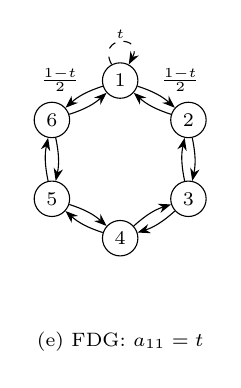
\begin{tikzpicture}[baseline=(c.base), scale=0.77]
    \foreach \i in {1,...,6} {
      \node[agent] (ra\i) at ({90-60*(\i-1)}:1.3) {\i};
    }
    \node (c) at (0,0) {};
    \foreach \i/\j in {2/3,3/4,4/5,5/6} {
      \draw[edge] (ra\i) to[bend left=12] (ra\j);
      \draw[edge] (ra\j) to[bend left=12] (ra\i);
    }
    \draw[edge] (ra2) to[bend left=12] (ra1);
    \draw[edge] (ra6) to[bend right=12] (ra1);
    \draw[edge] (ra1) to[bend left=12] node[weight, above right] {$\frac{1-t}{2}$} (ra2);
    \draw[edge] (ra1) to[bend right=12] node[weight, above left] {$\frac{1-t}{2}$} (ra6);
    % REVISED (2026-11-19, arrows: the dashed loop was narrow and hard to see). Was:
    % \draw[selfloop, dashed] (ra1) to node[weight, above] {$t$} (ra1);
    \draw[edge, dashed] (ra1) to[out=118, in=62, looseness=5, min distance=4mm]
      node[weight, above] {$t$} (ra1);
    \node at (0,-3.0) {\scriptsize (e) FDG: $a_{11} = t$};
  \end{tikzpicture}\hfill
  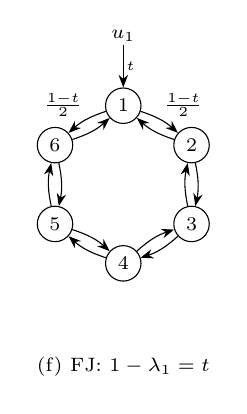
\begin{tikzpicture}[baseline=(c.base), scale=0.77]
    \foreach \i in {1,...,6} {
      \node[agent] (rb\i) at ({90-60*(\i-1)}:1.3) {\i};
    }
    \node (c) at (0,0) {};
    \foreach \i/\j in {2/3,3/4,4/5,5/6} {
      \draw[edge] (rb\i) to[bend left=12] (rb\j);
      \draw[edge] (rb\j) to[bend left=12] (rb\i);
    }
    \draw[edge] (rb2) to[bend left=12] (rb1);
    \draw[edge] (rb6) to[bend right=12] (rb1);
    \draw[edge] (rb1) to[bend left=12] node[weight, above right] {$\frac{1-t}{2}$} (rb2);
    \draw[edge] (rb1) to[bend right=12] node[weight, above left] {$\frac{1-t}{2}$} (rb6);
    \node[font=\scriptsize, inner sep=1pt] (urb1) at (90:2.45) {$u_1$};
    \draw[edge] (urb1) -- node[weight, right] {$t$} (rb1);
    \node at (0,-3.0) {\scriptsize (f) FJ: $1 - \lambda_1 = t$};
  \end{tikzpicture}\hfill
  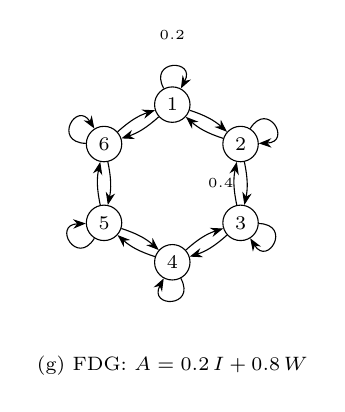
\begin{tikzpicture}[baseline=(c.base), scale=0.77]
    \foreach \i in {1,...,6} {
      \pgfmathsetmacro{\ang}{90-60*(\i-1)}
      \pgfmathsetmacro{\angout}{\ang+28}
      \pgfmathsetmacro{\angin}{\ang-28}
      \node[agent] (rc\i) at (\ang:1.3) {\i};
      \draw[edge] (rc\i) to[out=\angout, in=\angin, looseness=5, min distance=4mm] (rc\i);
    }
    \node (c) at (0,0) {};
    \foreach \i/\j in {1/2,2/3,3/4,4/5,5/6,6/1} {
      \draw[edge] (rc\i) to[bend left=12] (rc\j);
      \draw[edge] (rc\j) to[bend left=12] (rc\i);
    }
    \node[weight] at (90:2.45) {$0.2$};
    \node[weight] at (0:0.8) {$0.4$};
    \node at (0,-3.0) {\scriptsize (g) FDG: $A = 0.2\,I + 0.8\,W$};
  \end{tikzpicture}\hfill
  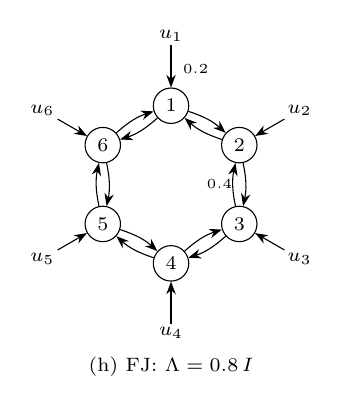
\begin{tikzpicture}[baseline=(c.base), scale=0.77]
    \foreach \i in {1,...,6} {
      \pgfmathsetmacro{\ang}{90-60*(\i-1)}
      \node[agent] (rd\i) at (\ang:1.3) {\i};
      \node[font=\scriptsize, inner sep=1pt] (urd\i) at (\ang:2.45) {$u_{\i}$};
      \draw[edge] (urd\i) -- (rd\i);
    }
    \node (c) at (0,0) {};
    \foreach \i/\j in {1/2,2/3,3/4,4/5,5/6,6/1} {
      \draw[edge] (rd\i) to[bend left=12] (rd\j);
      \draw[edge] (rd\j) to[bend left=12] (rd\i);
    }
    \node[weight] at (78:1.95) {$0.2$};
    \node[weight] at (0:0.8) {$0.4$};
    \node at (0,-3.0) {\scriptsize (h) FJ: $\Lambda = 0.8\,I$};
  \end{tikzpicture}

  \smallskip
  % REVISED (2026-11-22, notes of 22/11: the FJ panels draw the weights of Lambda W; panels
  % (e)-(h), so that they differ from those of the directed cycle). Was:
  % {\scriptsize Bidirectional ring of Figure~1(b). FJ model: $W = A(0)$, $u = x(0)$.
  % Unlabelled edges: weight $1/2$ in (a), (b) and $0.4$ in (c), (d), where every self-loop
  % and every prejudice has weight $0.2$. In (a), (b) agents $2$ and $6$ listen to agent~$1$
  % with weight $1/2$ for every $t$.\par}
  {\scriptsize Bidirectional ring of «Two networks, one agent». FJ model: $W = A(0)$, without self-loops,
  and $u = x(0)$. In (f), (h) the edges are those of $G$ and carry the weights of
  $\Lambda W$, $\lambda_i w_{ij}$: e.g.\ in (f) $w_{12} = \frac12$ and
  $\lambda_1 w_{12} = \frac{1-t}{2}$. The arrows from $u_i$, of weight $1 - \lambda_i$, are
  not edges of $G$. Unlabelled edges: weight $1/2$ in (e), (f) and $0.4$ in (g), (h), where
  every self-loop and every prejudice has weight $0.2$. In (e), (f) agents $2$ and $6$
  listen to agent~$1$ with weight $1/2$ for every $t$.\par}

  % MOVED (2026-11-22, layout): from m-fj-graphs; they hold for both networks.
  \smallskip
  \footnotesize
  \begin{itemize}
    \item Not a rewriting of one model as the other: the analogous FJ network, built to
          compare the two models.
    \item Only for $t = 1$, (b) and (f) are the rewritings of [5] of (a) and (e): $\lambda_1 = 0$,
          $u_1 = x_1(0)$, the same trajectories (Back to the question).
  \end{itemize}
\end{frame}

% ADDED (2026-11-17, preview): before the FJ examples, the two models on the networks of
% Figure 1, with the same weight on a different object (notes of 17/11).
% ADDED (2026-11-22, notes of 22/11: W and Lambda of the FJ model in matrix form, on their
% own slide, before the update equations; the report writes these matrices in Section 3.2.2:
% A(1/2) and Lambda W, A = 0.2 I + 0.8 W and Lambda W = 0.8 W).
% MOVED (2026-11-23, notes of 23/11: to backup.tex, to save time). Was:
% \begin{frame}[label=m-fj-matrices]{FJ on the same networks: $W$ and $\Lambda$}
%   \footnotesize
%   % REVISED (2026-11-22, notes of 22/11: W is the FDG matrix A(0), strongly connected and
%   % periodic). Was:
%   % $W = A(0)$: the networks of «Two networks, one agent», without self-loops. Prejudices
%   % $u = x(0) = (0, 0.2, \dots, 1)^\top$, as in the original FJ model.
%   $W = A(0)$: the networks of «Two networks, one agent», without self-loops, strongly
%   connected and periodic. With $\Lambda = I$ the FJ model is the FDG model with $A(0)$: the
%   opinions do not converge. Prejudices $u = x(0) = (0, 0.2, \dots, 1)^\top$, as in the
%   original FJ model.
%
%   {\setlength{\arraycolsep}{3.5pt}\renewcommand{\arraystretch}{0.8}%
%   \begin{columns}[c]
%     \column{0.44\textwidth}
%       \centering
%       Directed cycle: \
%       $W = \begin{bmatrix}
%         0&1&0&0&0&0\\ 0&0&1&0&0&0\\ 0&0&0&1&0&0\\ 0&0&0&0&1&0\\ 0&0&0&0&0&1\\ 1&0&0&0&0&0
%       \end{bmatrix}$
%     \column{0.52\textwidth}
%       \centering
%       Bidirectional ring: \
%       $W = \dfrac12 \begin{bmatrix}
%         0&1&0&0&0&1\\ 1&0&1&0&0&0\\ 0&1&0&1&0&0\\ 0&0&1&0&1&0\\ 0&0&0&1&0&1\\ 1&0&0&0&1&0
%       \end{bmatrix}$
%   \end{columns}}
%
%   \smallskip
%   \scriptsize
%   \renewcommand{\arraystretch}{1.1}
%   \begin{tabular}{@{}lllll@{}}
%     \toprule
%     & \textbf{FJ}: $\Lambda$ & $I - \Lambda$ & $\Lambda W$ & \textbf{FDG}: $A$ \\
%     \midrule
%     Agent~$1$ stubborn & $\operatorname{diag}(0, 1, \dots, 1)$
%       & $\operatorname{diag}(1, 0, \dots, 0)$ & $W$ with row~$1$ times $0$ & $A(1)$ \\
%     Agent~$1$ with weight $t$ & $\operatorname{diag}(1-t, 1, \dots, 1)$
%       & $\operatorname{diag}(t, 0, \dots, 0)$ & $W$ with row~$1$ times $1-t$ & $A(t)$ \\
%     Every agent with weight $0.2$ & $0.8\,I$ & $0.2\,I$ & $0.8\,W$ & $0.2\,I + 0.8\,W$ \\
%     \bottomrule
%   \end{tabular}
%
%   \smallskip
%   \footnotesize
%   \begin{itemize}
%     \setlength{\itemsep}{1pt}
%     \item $\Lambda W$ multiplies row~$i$ of $W$ by $\lambda_i$: its entries are the weights
%           on the edges of the FJ graphs (b), (d), (f), (h).
%     \item In the three cases $A$ and $\Lambda W$ have the same weights on the others. The rest of row~$i$,
%           $1 - \lambda_i$, is on the current opinion $x_i(k)$ in the FDG model (diagonal of
%           $A$), on the prejudice $u_i$ in the FJ model (out of the matrix):
%           $A = \Lambda W + (I - \Lambda)$.
%     % ADDED (2026-11-22, notes of 22/11: one prejudice is enough).
%     \item \alert{One prejudiced agent is enough}: $G$ is strongly connected, so every agent
%           has a path to agent~$1$ and is P-dependent; by Corollary~3.3 the FJ model is
%           asymptotically stable. No aperiodicity is needed. In the FDG model the same
%           change of one agent, a self-weight $t > 0$, gives consensus by making $G$
%           aperiodic.
%   \end{itemize}
% \end{frame}

% ADDED (2026-11-22, notes of 22/11: the matrices of the case «every agent with weight
% 0.2», as in the report, Section 3.2.2: A = 0.2 I + 0.8 W and Lambda W = 0.8 W).
% MOVED (2026-11-23, notes of 23/11: to backup.tex, to save time). Was:
% \begin{frame}[label=m-fj-matrices-all]{Every agent with weight $0.2$: the matrices}
%   \footnotesize
%   $\Lambda = 0.8\,I$, $I - \Lambda = 0.2\,I$, $u = x(0)$: every agent gives weight $0.2$ to
%   its current opinion in the FDG model, to its prejudice in the FJ model.
%   % ADDED (2026-11-22, notes of 22/11: why this case; report, Section 3.2.2).
%   \alert{Why this case:} with one prejudice the FJ model still reaches a consensus,
%   $u_1\mathbf{1}_6$; with a different prejudice for every agent it disagrees on the same
%   strongly connected network on which the FDG model can only agree. This is the main
%   difference between the two models.
%
%   \smallskip
%
%   \smallskip
%   {\setlength{\arraycolsep}{3pt}\renewcommand{\arraystretch}{0.85}\scriptsize
%   \begin{tabular}{@{}r@{\ \ }c@{\qquad}c@{}}
%     & \textbf{FDG}: $A = 0.2\,I + 0.8\,W$ & \textbf{FJ}: $\Lambda W = 0.8\,W$ \\ \noalign{\vskip 3pt}
%     directed cycle &
%     $\begin{bmatrix}
%       0.2&0.8&0&0&0&0\\ 0&0.2&0.8&0&0&0\\ 0&0&0.2&0.8&0&0\\ 0&0&0&0.2&0.8&0\\
%       0&0&0&0&0.2&0.8\\ 0.8&0&0&0&0&0.2
%     \end{bmatrix}$ &
%     $\begin{bmatrix}
%       0&0.8&0&0&0&0\\ 0&0&0.8&0&0&0\\ 0&0&0&0.8&0&0\\ 0&0&0&0&0.8&0\\
%       0&0&0&0&0&0.8\\ 0.8&0&0&0&0&0
%     \end{bmatrix}$ \\ \noalign{\vskip 6pt}
%     bidirectional ring &
%     $\begin{bmatrix}
%       0.2&0.4&0&0&0&0.4\\ 0.4&0.2&0.4&0&0&0\\ 0&0.4&0.2&0.4&0&0\\ 0&0&0.4&0.2&0.4&0\\
%       0&0&0&0.4&0.2&0.4\\ 0.4&0&0&0&0.4&0.2
%     \end{bmatrix}$ &
%     $\begin{bmatrix}
%       0&0.4&0&0&0&0.4\\ 0.4&0&0.4&0&0&0\\ 0&0.4&0&0.4&0&0\\ 0&0&0.4&0&0.4&0\\
%       0&0&0&0.4&0&0.4\\ 0.4&0&0&0&0.4&0
%     \end{bmatrix}$
%   \end{tabular}\par}
%
%   \footnotesize
%   \begin{itemize}
%     \setlength{\itemsep}{1pt}
%     \item $A$: row- and column-stochastic, i.e.\ doubly-stochastic, with a positive diagonal:
%           $G$ strongly connected and aperiodic, so consensus, with $w = \frac16\mathbf{1}_6$:
%           the average $0.5$ of $x(0)$.
%     \item $\Lambda W$: every row sums to $0.8$ (row-substochastic); every agent is
%           prejudiced, so all P-dependent: asymptotically stable, $x(\infty) = Vu$ (9).
%           The final opinions are closer to each other than the initial ones, but not
%           equal: the prejudices differ, so no consensus.
%   \end{itemize}
% \end{frame}

% REVISED (2026-11-22, notes of 22/11: the table did not show the entries of W, and the
% weight of the ring written as (1-t)(x_2(k) + x_6(k))/2 read as 1/2 instead of (1-t)/2.
% Now W is written out, and every cell is an update equation with the weight of each
% opinion written out, on both networks; W and Lambda in matrix form on the new slide
% m-fj-matrices, just before). Was:
% \begin{frame}[label=m-fj-networks]{FDG and FJ on the same networks}
%   \small
%   The networks of Figure~1 without self-loops, $W = A(0)$;
%   $x(0) = (0, 0.2, \dots, 1)^\top$; prejudices $u = x(0)$, as in the original FJ model.
%
%   \medskip
%   \scriptsize
%   \renewcommand{\arraystretch}{1.6}
%   \begin{tabular}{>{\raggedright\arraybackslash}p{0.19\textwidth}
%                   >{\raggedright\arraybackslash}p{0.36\textwidth}
%                   >{\raggedright\arraybackslash}p{0.37\textwidth}}
%     \toprule
%     & \textbf{FDG}: weight on the current opinion & \textbf{FJ}: weight on the prejudice \\
%     \midrule
%     Agent~$1$ stubborn (Figure~6) & $a_{11} = 1$: $A(1)$
%       & $\lambda_1 = 0$, $u_1 = x_1(0)$ \\
%     % REVISED (2026-11-19, notes of 19/11: the row of agent 1 written for both networks). Was:
%     % Agent~$1$ with weight $t$ (Figure~9: $t = 1/2$)
%     %   & $x_1(k+1) = t\,x_1(k) + (1-t)\textstyle\sum_j w_{1j}\,x_j(k)$
%     %   & $x_1(k+1) = (1-t)\textstyle\sum_j w_{1j}\,x_j(k) + t\,u_1$: $1 - \lambda_1 = t$ \\
%     Agent~$1$ with weight $t$ (Figure~9: $t = 1/2$)
%       & cycle: $x_1(k+1) = t\,x_1(k) + (1-t)\,x_2(k)$\newline
%         ring: $x_1(k+1) = t\,x_1(k) + (1-t)\,\bigl(x_2(k) + x_6(k)\bigr)/2$
%       & cycle: $x_1(k+1) = (1-t)\,x_2(k) + t\,u_1$\newline
%         ring: $x_1(k+1) = (1-t)\,\bigl(x_2(k) + x_6(k)\bigr)/2 + t\,u_1$\newline
%         $1 - \lambda_1 = t$ \\
%     Every agent with weight $0.2$ (Figure~10)
%       & $A = 0.2\,I + 0.8\,W$ & $\Lambda = 0.8\,I$ \\
%     \bottomrule
%   \end{tabular}
%
%   \smallskip
%   \footnotesize In the first two rows the other agents are as in $A(0)$ (FDG) and have
%   $\lambda_i = 1$ (FJ).
%   % ADDED (2026-11-19, notes of 19/11): the weights of the edges in the third row.
%   In the third row, networks (c), (d) and (g), (h), each edge weighs $0.8$ on the directed cycle and
%   $0.4$ on the bidirectional ring.
%   \socially{The same weight on a different object: the current opinion, which still moves
%   towards the others, or the prejudice, which never moves.}
% \end{frame}
% MOVED (2026-11-23, notes of 23/11: to backup.tex, to save time). Was:
% \begin{frame}[label=m-fj-networks]{FDG and FJ: the updates}
%   \footnotesize
%   Every cell is an update equation, with the weight of each opinion written out. In (5)
%   the weight of $x_j(k)$ in the update of agent~$i$ is $\lambda_i w_{ij}$, the entry
%   $(i,j)$ of $\Lambda W$.
%
%   \smallskip
%   \scriptsize
%   \renewcommand{\arraystretch}{1.3}
%   \begin{tabular}{@{}lll@{}}
%     \toprule
%     & \textbf{FDG}: self-weight $a_{ii}$ on the current opinion $x_i(k)$
%     & \textbf{FJ}: attachment $1 - \lambda_i$ to the prejudice $u_i$ \\
%     \midrule
%     \multicolumn{3}{@{}l}{\textbf{Agent~$1$ stubborn}: $a_{11} = 1$, $\lambda_1 = 0$
%       (Figure~6)} \\
%     both & $x_1(k+1) = x_1(k)$ & $x_1(k+1) = u_1 = x_1(0)$ \\
%     \midrule
%     \multicolumn{3}{@{}l}{\textbf{Agent~$1$ with weight $t$}: $a_{11} = t$,
%       $1 - \lambda_1 = t$ (graphs (a), (b), (e), (f); Figure~9: $t = \frac12$)} \\
%     cycle & $x_1(k+1) = t\,x_1(k) + (1-t)\,x_2(k)$
%       & $x_1(k+1) = (1-t)\,x_2(k) + t\,u_1$ \\
%     ring & $x_1(k+1) = t\,x_1(k) + \frac{1-t}{2}\,x_2(k) + \frac{1-t}{2}\,x_6(k)$
%       & $x_1(k+1) = \frac{1-t}{2}\,x_2(k) + \frac{1-t}{2}\,x_6(k) + t\,u_1$ \\
%     \midrule
%     \multicolumn{3}{@{}l}{\textbf{Every agent with weight $0.2$}: $A = 0.2\,I + 0.8\,W$,
%       $\Lambda = 0.8\,I$ (graphs (c), (d), (g), (h); Figure~10)} \\
%     cycle & $x_i(k+1) = 0.2\,x_i(k) + 0.8\,x_{i+1}(k)$
%       & $x_i(k+1) = 0.8\,x_{i+1}(k) + 0.2\,u_i$ \\
%     ring & $x_i(k+1) = 0.2\,x_i(k) + 0.4\,x_{i-1}(k) + 0.4\,x_{i+1}(k)$
%       & $x_i(k+1) = 0.4\,x_{i-1}(k) + 0.4\,x_{i+1}(k) + 0.2\,u_i$ \\
%     \bottomrule
%   \end{tabular}
%
%   \smallskip
%   \footnotesize In the first two cases the other agents are as in $A(0)$ in both models
%   ($\lambda_i = 1$).
%   \socially{The same weight on a different object: the current opinion, which still moves
%   towards the others, or the prejudice, which never moves.}
% \end{frame}

\begin{frame}[label=m-state-input]{Stubborn agent: state or input}
  \begin{columns}[T]
    \column{0.58\textwidth}
      \centering
      % REVISED (2026-11-11, terms: the FDG model with A(1) is convergent but not
      % asymptotically stable; captions with all the parameters). Was:
      % \only<1>{\includegraphics[width=\linewidth]{fj_stubborn_equivalence.eps}
      %
      % {\scriptsize Figure 6. Left: FDG with $A(1)$; right: FJ with $\lambda_1 = 0$,
      % $u = x(0)$.}}%
      % \only<2>{\includegraphics[width=\linewidth]{fj_stubborn_perturbation.eps}
      %
      % {\scriptsize Figure 7. Same models from $x_1(0) = 0.5$, $u$ unchanged.}}
      % \column{0.40\textwidth}
      %   \footnotesize
      %   \only<1>{%
      %   \begin{itemize}
      %     \item Rewriting [5]: $\lambda_i = 0$, $u_i = x_i(0)$ for the stubborn agents,
      %           $\lambda_i = 1$ for the others.
      %     \item \alert{Same trajectories}, not the same stability: FDG never
      %           asymptotically stable (eigenvalue $1$), FJ asymptotically stable
      %           (Corollary~3.3).
      %   \end{itemize}}%
      %   \only<2>{%
      %   \begin{itemize}
      %     \item FDG: agent~$1$ keeps $0.5$, the group follows it: never forgotten.
      %     \item FJ: agent~$1$ back to $u_1 = 0$ after one step, same limit $Vu$.
      %     \item Stubborn row: $e_1^\top$ in $A(1)$, $0$ in $\Lambda W$: the eigenvalue
      %           $1$ becomes $0$.
      %   \end{itemize}}
      \only<1>{\includegraphics[width=\linewidth]{fj_stubborn_equivalence.eps}

      {\scriptsize Figure 6. Left: FDG model with $A(1)$; right: FJ model with
      $\lambda_1 = 0$, $\lambda_i = 1$ for $i \neq 1$, $u = x(0)$.}}%
      \only<2>{\includegraphics[width=\linewidth]{fj_stubborn_perturbation.eps}

      {\scriptsize Figure 7. The same models from $x_1(0) = 0.5$, with $u$ unchanged.
      % ADDED (2026-11-22, notes of 22/11).
      \par\smallskip\textit{Note: in the FJ model agent~$1$ is no longer stubborn here:
      $\lambda_1 = 0$, but $u_1 = 0 \neq x_1(0) = 0.5$.}}}
    \column{0.40\textwidth}
      \footnotesize
      \only<1>{%
      \begin{itemize}
        \item Rewriting [5]: $\lambda_i = 0$, $u_i = x_i(0)$ for the stubborn agents,
              $\lambda_i = 1$ (any $u_i$) for the others.
        \item \alert{Same trajectories}, not the same stability: the FDG model is
              convergent but never asymptotically stable ($1 \in \operatorname{spec}(A)$,
              Theorem~1.6); the FJ model is asymptotically stable (Corollary~3.3).
      \end{itemize}}%
      \only<2>{%
      \begin{itemize}
        % REVISED (2026-11-19, notes of 19/11: what the two limits contain). Was:
        % \item FDG: agent~$1$ keeps $0.5$ and the group follows it: never forgotten.
        % \item FJ: agent~$1$ goes back to $u_1 = 0$ at the first step; same limit $Vu$.
        \item FDG: agent~$1$ keeps $0.5$ and the group follows it: the limit
              $x_1(0)\,\mathbf{1}_6$ ($w = e_1$) becomes $0.5\,\mathbf{1}_6$, never
              forgotten.
        \item FJ: agent~$1$ goes back to $u_1 = 0$ at the first step; the limit
              $x(\infty) = Vu$ does not contain $x(0)$: the same limit.
        \item Row of agent~$1$: $e_1^\top$ in $A(1)$, zero in $\Lambda W$: the eigenvalue
              $1$ of $A(1)$ becomes $0$ in $\Lambda W$.
      \end{itemize}}
      \vspace{1mm}
      % REVISED (2026-11-22, notes of 22/11: an unperturbed stubborn agent forgets nothing;
      % the difference is where its opinion is stored, seen when x(0) is moved). Was (as in
      % the report, Section 3.2.2):
      % \sociallycol{In the FDG model stubbornness is a memory in the state, never forgotten;
      % in the FJ model it is an external input, and the state forgets $x(0)$.}
      % REMOVED (2026-11-22, notes of 22/11: stubbornness in the FJ model is a condition on
      % both lambda_1 and u_1 = x_1(0); moving only x_1(0), agent 1 is no longer stubborn).
      % Was:
      % \sociallycol{In the FDG model the stubborn opinion is in the state: move it, and the
      % group follows. In the FJ model it is a fixed prejudice: move the state, and the group
      % ends where it did.}
  \end{columns}
  \detailbuttons{\go{bk-state-input}{Spectra}\ \go{bk-rewritings}{Rewritings}}
\end{frame}

% ADDED (2026-11-16, notes): the answer to the question of the slide m-bridge, with the
% second rewriting of the report (Section 3.2.1, Figure 8, there with agent 1 only)
% applied to the two stubborn agents. Both readings give the same trajectories.
% MOVED (2026-11-17, preview): the frame m-back-question is now right after
% m-fj-final (the augmented model, read backwards, gives the answer).

\begin{frame}[label=m-one-prej]{A single prejudice}
  \begin{columns}[T]
    \column{0.58\textwidth}
      \centering
      \includegraphics[width=\linewidth]{fj_one_prejudiced.eps}

      % REVISED (2026-11-11, terms: why all agents are P-dependent; "anchor" only in the
      % green block). Was:
      % {\scriptsize Figure 9. Weight $1/2$ on agent~$1$. Left: FDG $A(1/2)$; right: FJ
      % $1 - \lambda_1 = 1/2$.}
      % \column{0.40\textwidth}
      %   \footnotesize
      %   \begin{itemize}
      %     \item All P-dependent: FJ \alert{asymptotically stable on a periodic network},
      %           with no self-loop.
      %     \item $V = \mathbf{1}_6 e_1^\top$: $x(\infty) = u_1\mathbf{1}_6 = 0$ for every
      %           $1 - \lambda_1 > 0$; FDG stops at $3/7$.
      %     \item $c = e_1$: one anchor takes \alert{all} the influence centrality, against
      %           $w_1 = 2/7$.
      %   \end{itemize}
      {\scriptsize Figure 9. Weight $1/2$ on agent~$1$. Left: FDG model with $A(1/2)$;
      right: FJ model with $\lambda_1 = 1/2$, $\lambda_i = 1$ for $i \neq 1$,
      $u = x(0)$.}

      % ADDED (2026-11-18, notes of 18/11): why there is no figure for the other two
      % values of the attachment (as in the report, paragraph "A single prejudice").
      \smallskip
      {\scriptsize The other two values need no new figure: $1 - \lambda_1 = 0$ is the FDG
      model with $A(0)$ (Figure~2, $t = 0$), $1 - \lambda_1 = 1$ is agent~$1$ stubborn
      (Figure~6).}
    \column{0.40\textwidth}
      \footnotesize
      \begin{itemize}
        \item Strongly connected network: all agents P-dependent, \alert{asymptotically
              stable} (Corollary~3.3), although $G$ is periodic and has no self-loop.
        \item FJ: $V = \mathbf{1}_6 e_1^\top$, $x(\infty) = u_1\mathbf{1}_6 = 0$ for every
              attachment $1 - \lambda_1 > 0$. FDG: consensus value $3/7$.
        \item $c = e_1$ for every $\lambda_1 < 1$: agent~$1$ takes \alert{all} the
              influence centrality; in the FDG model, $w_1 = 2/7$ at $t = 1/2$.
      \end{itemize}
      \vspace{1mm}
      \sociallycol{One anchored agent that influences everybody decides where the whole group
  ends, however weak its attachment.}
  \end{columns}
  \detailbuttons{\go{bk-one-prej}{Matrices}}
\end{frame}

\begin{frame}[label=m-all-prej]{Every agent prejudiced}
  \begin{columns}[T]
    \column{0.58\textwidth}
      \centering
      \includegraphics[width=\linewidth]{fj_all_prejudiced.eps}

      % REVISED (2026-11-17, preview: the same attachment, different prejudices). Was:
%       {\scriptsize Figure 10. Weight $0.2$ for all. Left: FDG $A = 0.2I + 0.8W$; right:
%       FJ $\Lambda = 0.8I$, $u = x(0)$.}
      {\scriptsize Figure 10. Weight $0.2$ for all. Left: FDG $A = 0.2I + 0.8W$; right:
      FJ $\Lambda = 0.8I$, $u = x(0)$: the same attachment for every agent, different
      prejudices.}
    \column{0.40\textwidth}
      \footnotesize
      % REVISED (2026-11-11, terms: the results used; the FJ disagreement as case (iv) of
      % the augmented graph). Was:
      % \begin{itemize}
      %   \item FDG: primitive, doubly stochastic: \alert{consensus} on the average $0.5$
      %         (Corollary~2.3).
      %   \item FJ: $V = 0.2\,(I - 0.8W)^{-1} > 0$: every prejudice in every final opinion,
      %         with different weights: \alert{disagreement}.
      %   \item Strongly connected: FDG never disagrees; the FJ disagreement comes from the
      %         prejudices.
      % \end{itemize}
      \begin{itemize}
        \item FDG: $A$ primitive (Corollary~1.12), doubly-stochastic: \alert{consensus}
              on the average $0.5$ (Corollary~2.3).
        \item FJ: $\Lambda < I_6$, asymptotically stable (Corollary~3.3);
              $V = 0.2\,(I - 0.8W)^{-1}$ has all entries positive. The prejudices differ:
              \alert{disagreement}.
        % REVISED (2026-11-16, notes: the augmented graph of this example has its own
        % slide, m-six-sinks). Was:
        % \item Strongly connected: the FDG model never disagrees; the FJ disagreement comes
        %       from the prejudices, case (iv) of the augmented graph (Remark~2.7).
        \item Strongly connected: the FDG model never disagrees; the FJ disagreement comes
              from the prejudices (next slide).
      \end{itemize}
      \vspace{1mm}
      \sociallycol{Inertia gives way in the end, an anchor does not: different anchors keep the
  group divided, a cleavage of opinions [5].}
  \end{columns}
  \detailbuttons{\go{bk-all-prej}{Matrices}\ \go{m-six-sinks}{Six sinks}}
\end{frame}

% ADDED (2026-11-16, notes): the FJ model of Figure 10 as an FDG model on the augmented
% graph (11): six sinks, case (iv) of Table 1, the disagreement of Theorem 2.4 and
% Remark 2.7. The report says it after Figure 10 (Section 3.2.2): "In the augmented
% graph the six prejudices are six stubborn virtual agents with different opinions, as
% in Remark 2.7". Reason 3 for not simulating a disagreement in the FDG part.
% REVISED (2026-11-16, notes): the two graphs drawn larger, side by side and with the
% same layout, so that the condensation digraph is the augmented graph with the real
% agents collapsed into one node; the chain one, two, six stubborn agents. Was:
% \begin{frame}[label=m-six-sinks]{Six prejudices, six sinks}
%   \compactblocks
%   \begin{columns}[T]
%     \column{0.42\textwidth}
%       \centering
%       \begin{tikzpicture}[baseline=(c.base), scale=0.45]
%         \foreach \i in {1,...,6} {
%           \pgfmathsetmacro{\ang}{90-60*(\i-1)}
%           \pgfmathsetmacro{\angout}{\ang+28}
%           \pgfmathsetmacro{\angin}{\ang-28}
%           \node[agent] (g\i) at (\ang:1.15) {\i};
%           \node[agent, dashed, minimum size=5.5mm] (v\i) at (\ang:2.45) {\i$'$};
%           \draw[edge] (g\i) -- (v\i);
%           \draw[edge] (v\i) to[out=\angout, in=\angin, looseness=5, min distance=4mm]
%             (v\i);
%         }
%         \node (c) at (0,0) {};
%         \foreach \i/\j in {1/2,2/3,3/4,4/5,5/6,6/1} {
%           \draw[edge] (g\i) -- (g\j);
%         }
%       \end{tikzpicture}
%
%       {\scriptsize (a) Augmented graph of the directed cycle.}
%
%       \vspace{1mm}
%       \begin{tikzpicture}[scale=0.45]
%         \node[draw, rounded corners=2pt, font=\scriptsize, inner sep=2pt] (R) at (0,0)
%           {$\{1, \dots, 6\}$};
%         \foreach \i in {1,...,6} {
%           \node[agent, dashed, minimum size=5.5mm] (c\i) at ({-3.4+1.36*(\i-1)},-1.5)
%             {\i$'$};
%           \draw[edge] (R) -- (c\i);
%         }
%       \end{tikzpicture}
%
%       {\scriptsize (b) Its condensation digraph, the same on the ring.}
%     \column{0.56\textwidth}
%       \footnotesize
%       \begin{itemize}
%         \item Figure~10, $\Lambda = 0.8I$: each real agent $i$ listens with weight $0.2$ to
%               its virtual agent $i'$, stubborn at $u_i$, and with total weight $0.8$ to
%               the other real agents: an FDG model on $12$ agents (11).
%         \item $C(\bar G)$: the real agents form one strongly connected component, not a
%               sink; the virtual agents are six sinks, aperiodic because of their
%               self-loops. Theorem~2.4 with $n_s = 6$: \alert{case (iv)}, as in
%               Remark~2.7.
%         \item Real agents: $x(\infty) = Vu$, $V = 0.2\,(I - 0.8W)^{-1}$ with all entries
%               positive: every final opinion is a convex combination of all six prejudices.
%         \item Figure~9 also has six sinks, but only $1'$ is listened to: without the
%               other five, a single sink and a consensus.
%       \end{itemize}
%       \begin{minipage}{0.80\linewidth}
%         \begin{alertblock}{The FDG disagreement, not forgotten}
%           \footnotesize The augmented FJ model is an FDG model: here its disagreement
%           appears, with all six sinks listened to.
%         \end{alertblock}
%       \end{minipage}
%   \end{columns}
%   \detailbuttons{\go{bk-augmented}{Augmented}}
% \end{frame}

% REVISED (2026-11-18, notes of 18/11): the augmented graph had no room for its arrows
% (real agents at radius 0.57 cm). Now the graph has its own column, with the same layout
% as network (d) of m-fj-graphs; the text goes to the right column in three steps: the
% sinks (with the condensation digraph), the consequences, the twelve trajectories.
% Was:
% \begin{frame}[label=m-six-sinks]{Six prejudices, six sinks}
%   \compactblocks
%   \begin{columns}[T]
%     \column{0.64\textwidth}
%       \centering
%       \begin{tikzpicture}[scale=0.52]
%         % (a) augmented graph of the directed cycle, Lambda = 0.8 I
%         \fill[red_unipd!10] (0,0) circle (1.7);
%         \foreach \i in {1,...,6} {
%           \pgfmathsetmacro{\ang}{90-60*(\i-1)}
%           \node[agent, fill=white] (g\i) at (\ang:1.1) {\i};
%           \node[agent, dashed, fill=white, minimum size=5.5mm] (v\i) at (\ang:2.6)
%             {\i$'$};
%         }
%         \foreach \i/\j in {1/2,3/4,4/5,5/6,6/1} {
%           \draw[edge] (g\i) -- (g\j);
%         }
%         \draw[edge] (g2) -- node[weight, right] {$0.8$} (g3);
%         \foreach \i in {2,...,6} {
%           \draw[edge] (g\i) -- (v\i);
%         }
%         \draw[edge] (g1) -- node[weight, left] {$0.2$} (v1);
%         \foreach \i in {2,...,6} {
%           \pgfmathsetmacro{\ang}{90-60*(\i-1)}
%           \pgfmathsetmacro{\angout}{\ang+28}
%           \pgfmathsetmacro{\angin}{\ang-28}
%           \draw[edge] (v\i) to[out=\angout, in=\angin, looseness=5, min distance=4mm]
%             (v\i);
%         }
%         \draw[edge] (v1) to[out=118, in=62, looseness=5, min distance=4mm]
%           node[weight, above] {$1$} (v1);
%         \node at (0,-4.0) {\scriptsize (a) augmented graph};
%         % arrow
%         \node at (4.15,0) {\Large $\Rightarrow$};
%         \node[font=\tiny, align=center] at (4.15,-0.85) {collapse the\\ component};
%         % (b) condensation digraph, same layout
%         \begin{scope}[shift={(8.3,0)}]
%           \node[circle, fill=red_unipd!10, draw=red_unipd, inner sep=1pt,
%                 minimum size=1.55cm, font=\scriptsize] (R) at (0,0) {$\{1,\dots,6\}$};
%           \foreach \i in {1,...,6} {
%             \pgfmathsetmacro{\ang}{90-60*(\i-1)}
%             \node[agent, dashed, minimum size=5.5mm] (w\i) at (\ang:2.6) {\i$'$};
%             \draw[edge] (R) -- (w\i);
%           }
%           \node at (0,-4.0) {\scriptsize (b) condensation digraph: six sinks};
%         \end{scope}
%       \end{tikzpicture}
%     \column{0.34\textwidth}
%       \footnotesize
%       Figure~10 ($\Lambda = 0.8I$) as an FDG model on $12$ agents (11): total weight $0.8$
%       to the other real agents, $0.2$ to the virtual agent $i'$, stubborn at $u_i$.
%
%       \medskip
%       Real agents: one strongly connected component (shaded), not a sink. Virtual agents:
%       six sinks, aperiodic because of their self-loops.
%
%       \medskip
%       Theorem~2.4 with $n_s = 6$: \alert{case (iv)}, as in Remark~2.7. The same on the
%       bidirectional ring.
%   \end{columns}
%   % (old bottom row, kept as history)
%   % \vspace{1mm}
%   % \begin{columns}[T, totalwidth=0.88\textwidth]
%   % \column{0.43\textwidth}
%   % \footnotesize
%   % \begin{itemize}
%   % \item $x(\infty) = Vu$, $V = 0.2\,(I - 0.8W)^{-1}$ with all entries positive:
%   % every final opinion is a convex combination of all six prejudices.
%   % \item Figure~9: six sinks too, but only $1'$ is listened to; without the other
%   % five, a single sink and a consensus.
%   % \end{itemize}
%   % \column{0.43\textwidth}
%   % \begin{alertblock}{The FDG disagreement, not forgotten}
%   % \footnotesize One stubborn agent: consensus (Figure~2, $t = 1$). Two: disagreement
%   % (the bridge). Six virtual ones, all listened to: here, an FDG model with the
%   % disagreement of Theorem~2.4.
%   % \end{alertblock}
%   % \end{columns}
%   % \detailbuttons{\go{bk-augmented}{Augmented}}
%   % \end{frame}
%   % REVISED (2026-11-16, notes: two steps; the twelve trajectories of the augmented model
%   % and why every real agent leaves the line of its virtual agent; the chain with the
%   % slide titles). Was: the bottom row of step 1 only, with "(the bridge)".
%   \only<1>{%
%   \begin{columns}[T, totalwidth=0.88\textwidth]
%     \column{0.43\textwidth}
%       \footnotesize
%       \begin{itemize}
%         \item $x(\infty) = Vu$, $V = 0.2\,(I - 0.8W)^{-1}$ with all entries positive:
%               every final opinion is a convex combination of all six prejudices.
%         \item Figure~9: six sinks too, but only $1'$ is listened to; without the other
%               five, a single sink and a consensus.
%       \end{itemize}
%     \column{0.43\textwidth}
%       \begin{alertblock}{The FDG disagreement, not forgotten}
%         \footnotesize One stubborn agent: consensus (Figure~2, $t = 1$). Two:
%         disagreement (Two stubborn agents; Back to the question). Six virtual ones, all
%         listened to: here, an FDG model with the disagreement of Theorem~2.4.
%       \end{alertblock}
%   \end{columns}}%
%   \only<2>{%
%   \begin{minipage}{0.84\textwidth}
%     \footnotesize
%     \textbf{Twelve trajectories.} Figure~10 shows only the six real agents; in the
%     augmented model the six virtual agents stay at $u_i = x_i(0)$. Every real agent starts
%     on the line of its virtual agent and leaves it as soon as the opinions it listens to
%     (weight $0.8$) average to a different value: at once on the directed cycle; on the
%     ring, agents $2, \dots, 5$ later, when the change of agents $1$ and $6$ reaches them.
%     The weight $0.2$ on its virtual agent keeps pulling it back, and it settles at
%     $x(\infty) = Vu$, never on its own prejudice. In the FDG model the same $0.2$ is on
%     the current opinion: the agent follows the group to the consensus.
%   \end{minipage}}
%   \detailbuttons{\go{bk-augmented}{Augmented}}
% \end{frame}
% MOVED (2026-11-23, notes of 23/11: to backup.tex, to save time). Was:
% \begin{frame}[label=m-six-sinks,t]{Six prejudices, six sinks}
%   % [t]: the augmented graph does not move between the three steps
%   \compactblocks
%   \begin{columns}[T]
%     \column{0.36\textwidth}
%       \centering
%       \begin{tikzpicture}[scale=0.7]
%         \fill[red_unipd!10] (0,0) circle (1.85);
%         \foreach \i in {1,...,6} {
%           \pgfmathsetmacro{\ang}{90-60*(\i-1)}
%           \node[agent, fill=white] (g\i) at (\ang:1.3) {\i};
%           \node[agent, dashed, fill=white, minimum size=5mm] (v\i) at (\ang:2.6) {\i$'$};
%         }
%         \foreach \i/\j in {1/2,3/4,4/5,5/6,6/1} {
%           \draw[edge] (g\i) -- (g\j);
%         }
%         \draw[edge] (g2) -- node[weight, left] {$0.8$} (g3);
%         \foreach \i in {2,...,6} {
%           \draw[edge] (g\i) -- (v\i);
%         }
%         \draw[edge] (g1) -- node[weight, left] {$0.2$} (v1);
%         \foreach \i in {2,...,6} {
%           \pgfmathsetmacro{\ang}{90-60*(\i-1)}
%           \pgfmathsetmacro{\angout}{\ang+28}
%           \pgfmathsetmacro{\angin}{\ang-28}
%           \draw[edge] (v\i) to[out=\angout, in=\angin, looseness=5, min distance=4mm]
%             (v\i);
%         }
%         \draw[edge] (v1) to[out=118, in=62, looseness=5, min distance=4mm]
%           node[weight, right] {$1$} (v1);
%         \node at (0,-3.85) {\scriptsize (a) augmented graph of network (d)};
%       \end{tikzpicture}
%     \column{0.62\textwidth}
%       \footnotesize
%       \only<1>{%
%         {\centering
%           \begin{tikzpicture}[scale=0.62]
%             \node[circle, fill=red_unipd!10, draw=red_unipd, inner sep=0pt,
%                   minimum size=1.15cm, font=\scriptsize] (R) at (0,0) {$\{1,\dots,6\}$};
%             \foreach \i in {1,...,6} {
%               \pgfmathsetmacro{\ang}{90-60*(\i-1)}
%               \node[agent, dashed, minimum size=5mm] (w\i) at (\ang:1.85) {\i$'$};
%               \draw[edge] (R) -- (w\i);
%             }
%             \node[anchor=west, font=\scriptsize] at (2.7,0)
%               {(b) condensation digraph: six sinks};
%           \end{tikzpicture}\par}
%         \smallskip
%         Network (d) ($\Lambda = 0.8I$, Figure~10) as an FDG model on $12$ agents (11):
%         each prejudice $u_i$ becomes the virtual agent $i'$, stubborn at $u_i$; agent $i$
%         gives $0.8$ to the other real agents and $0.2$ to $i'$.
%
%         \smallskip
%         Real agents: one strongly connected component (shaded), not a sink. Virtual
%         agents: six sinks, aperiodic because of their self-loops.
%
%         \smallskip
%         Theorem~2.4 with $n_s = 6$: \alert{case (iv)}, as in Remark~2.7. The same on the
%         bidirectional ring.}%
%       \only<2>{%
%         \begin{itemize}
%           \item $x(\infty) = Vu$, $V = 0.2\,(I - 0.8W)^{-1}$ with all entries positive:
%                 every final opinion is a convex combination of all six prejudices.
%           \item Figure~9: six sinks too, but only $1'$ is listened to; without the other
%                 five, a single sink and a consensus.
%         \end{itemize}
%         \begin{alertblock}{The FDG disagreement, not forgotten}
%           \footnotesize One stubborn agent: consensus (Figure~2, $t = 1$). Two:
%           disagreement (Two stubborn agents; Back to the question). Six virtual ones, all
%           listened to: here, an FDG model with the disagreement of Theorem~2.4.
%         \end{alertblock}}%
%       \only<3>{%
%         \textbf{Twelve trajectories.} Figure~10 shows only the six real agents; in the
%         augmented model the six virtual agents stay at $u_i = x_i(0)$. Every real agent
%         starts on the line of its virtual agent and leaves it as soon as the opinions it
%         listens to (weight $0.8$) average to a different value: at once on the directed
%         cycle; on the ring, agents $2, \dots, 5$ later, when the change of agents $1$ and
%         $6$ reaches them. The weight $0.2$ on its virtual agent keeps pulling it back, and
%         it settles at $x(\infty) = Vu$, never on its own prejudice. In the FDG model the
%         same $0.2$ is on the current opinion: the agent follows the group to the
%         consensus.}
%   \end{columns}
%   \detailbuttons{\go{bk-augmented}{Augmented}}
% \end{frame}

% REVISED (2026-11-17, preview): three examples, each with what we expect (step 1),
% then the results (step 2). Was:
% \begin{frame}[label=m-aux]{Where no prejudice arrives}
%   % REVISED (2026-11-11, terms: the closed group is a sink of C(G)). Was:
%   % Agents $1, 2, 3$ form a closed group, agents $4, 5, 6$ a chain that listens to it. One
%   % prejudiced agent, $\lambda = 0.5$. P-dependent agents shaded.
%   \only<1>{%
%   \small
%   Agents $1, 2, 3$ form a closed group (a sink of $C(G)$), agents $4, 5, 6$ a chain that
%   listens to it. One prejudiced agent, $\lambda = 0.5$. P-dependent agents shaded.
%
%   \vspace{3mm}
%   \centering
%   \begin{tikzpicture}[scale=0.6, every node/.append style={transform shape}, pdep/.style={agent, fill=gray!30}]
%     \begin{scope}
%       \node[pdep] (a1) at (0,1.1) {1}; \node[pdep] (a2) at (-1.1,-0.5) {2};
%       \node[pdep] (a3) at (1.1,-0.5) {3}; \node[pdep] (a6) at (2.4,1.1) {6};
%       \node[pdep] (a5) at (3.8,1.1) {5}; \node[pdep] (a4) at (5.1,1.1) {4};
%       \draw[edge] (a1) -- (a2); \draw[edge] (a2) -- node[weight, below] {$0.5$} (a3); \draw[edge] (a3) -- (a1);
%       \draw[edge] (a4) -- (a5); \draw[edge] (a5) -- (a6); \draw[edge] (a6) -- (a1);
%       \draw[edge] (-1.1,-1.8) node[below, font=\scriptsize] {$u_2$} -- node[weight, left] {$0.5$} (a2);
%       \node[font=\normalsize] at (2.0,-2.9) {(a) $W_{\mathrm{p}}$, agent~$2$ prejudiced};
%     \end{scope}
%     \begin{scope}[xshift=8.3cm]
%       \node[agent] (a1) at (0,1.1) {1}; \node[agent] (a2) at (-1.1,-0.5) {2};
%       \node[agent] (a3) at (1.1,-0.5) {3}; \node[agent] (a6) at (2.4,1.1) {6};
%       \node[pdep] (a5) at (3.8,1.1) {5}; \node[pdep] (a4) at (5.1,1.1) {4};
%       \draw[edge] (a1) -- (a2); \draw[edge] (a2) -- (a3); \draw[edge] (a3) -- (a1);
%       \draw[edge] (a4) -- (a5); \draw[edge] (a5) -- node[weight, above] {$0.5$} (a6); \draw[edge] (a6) -- (a1);
%       \draw[edge] (3.8,2.4) node[above, font=\scriptsize] {$u_5$} -- node[weight, right] {$0.5$} (a5);
%       \node[font=\normalsize] at (2.0,-2.9) {(b) $W_{\mathrm{p}}$, agent~$5$ prejudiced};
%     \end{scope}
%     \begin{scope}[xshift=16.6cm]
%       \node[agent] (a1) at (0,1.1) {1}; \node[agent] (a2) at (-1.1,-0.5) {2};
%       \node[agent] (a3) at (1.1,-0.5) {3}; \node[agent] (a6) at (2.4,1.1) {6};
%       \node[pdep] (a5) at (3.8,1.1) {5}; \node[pdep] (a4) at (5.1,1.1) {4};
%       \draw[edge] (a1) to[bend left=20] (a2);
%       \draw[edge] (a2) -- node[weight, below] {$1/2$} (a3); \draw[edge] (a3) -- (a1);
%       \draw[edge] (a2) to[bend left=20] node[weight, below right] {$1/2$} (a1);
%       \draw[edge] (a4) -- (a5); \draw[edge] (a5) -- node[weight, above] {$0.5$} (a6); \draw[edge] (a6) -- (a1);
%       \draw[edge] (3.8,2.4) node[above, font=\scriptsize] {$u_5$} -- node[weight, right] {$0.5$} (a5);
%       \node[font=\normalsize] at (2.0,-2.9) {(c), (d) $W_{\mathrm{a}}$, agent~$5$ prejudiced};
%     \end{scope}
%   \end{tikzpicture}
%
%   \vspace{3mm}
%   \raggedright
%   {\small In $W_{\mathrm{p}}$ the closed group is a periodic cycle; in $W_{\mathrm{a}}$
%   the edge $2 \to 1$ makes it aperiodic. In (d) only $x_2(0)$ moves, from $0.5$ to $1$.}
%
%   \vspace{2mm}
%   {\scriptsize Figure 11.}
%   }%
%   \only<2>{%
%   \begin{columns}[T]
%     \column{0.54\textwidth}
%       \centering
%       \includegraphics[width=\linewidth]{fj_auxiliary.eps}
%
%       {\scriptsize Figure 12. $u = (0,\, 0.5,\, 1,\, 0.2,\, 0.9,\, 0.6)^\top$.}
%     \column{0.44\textwidth}
%       \footnotesize
%       % REVISED (2026-11-11, terms: the result behind each panel; "remembers" only in the
%       % green block). Was:
%       % \begin{itemize}
%       %   \item[(a)] Prejudice in the closed group: \alert{asymptotically stable}, all at
%       %         $0.5$.
%       %   \item[(b)] Outside, periodic closed group: $W^{22}$ not regular, \alert{no
%       %         convergence}.
%       %   \item[(c)] Aperiodic: \alert{convergent, not asymptotically stable}; $1,2,3,6$ at
%       %         $0.4$, $4,5$ at $0.65$.
%       %   \item[(d)] $x_2(0) = 1$: $0.6$ and $0.75$: the closed group \alert{remembers}.
%       % \end{itemize}
%       \begin{itemize}
%         \item[(a)] Agent~$2$ in the closed group, $r = n$: \alert{asymptotically stable}
%               (Corollary~3.3), all at $u_2 = 0.5$, although the cycle is periodic.
%         \item[(b)] $r = 2$: the closed group $\{1,2,3\}$ is periodic, so $W^{22}$ is not
%               regular: \alert{not convergent} (Theorem~3.2).
%         \item[(c)] $W^{22}$ regular: \alert{convergent} (Theorem~3.2), \alert{not
%               asymptotically stable} (Corollary~3.3); $1,2,3,6$ at $0.4$, $4,5$ at $0.65$.
%         \item[(d)] $x_2(0) = 1$, $u$ unchanged: $0.6$ and $0.75$. The limit depends on the
%               initial opinions of the P-independent agents.
%       \end{itemize}
%       \vspace{1mm}
%       \sociallycol{Agents that no prejudice reaches form an FDG model of their own: they need
%   aperiodicity and remember their initial opinions.}
%   \end{columns}}
%   \detailbuttons{\go{bk-aux}{Blocks}\ \go{bk-aux-table}{Table 2}}
% \end{frame}
\begin{frame}[label=m-aux]{Where no prejudice arrives}
  \only<1>{%
  \small
  Agents $1, 2, 3$ form a closed group (a sink of $C(G)$), agents $4, 5, 6$ a chain that
  listens to it. One prejudiced agent, $\lambda = 0.5$. P-dependent agents shaded.

  \centering
  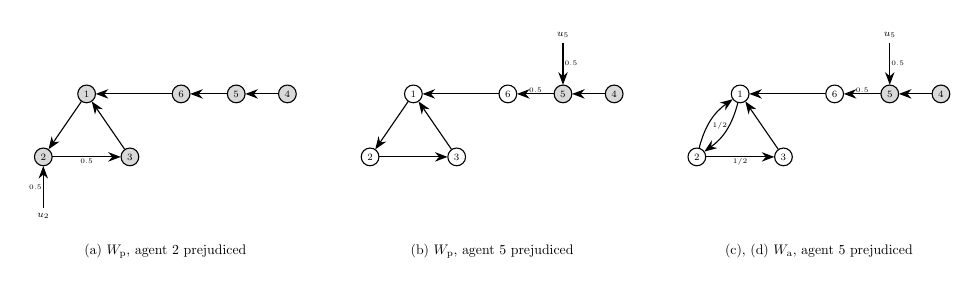
\begin{tikzpicture}[scale=0.5, every node/.append style={transform shape}, pdep/.style={agent, fill=gray!30}]
    \begin{scope}
      \node[pdep] (a1) at (0,1.1) {1}; \node[pdep] (a2) at (-1.1,-0.5) {2};
      \node[pdep] (a3) at (1.1,-0.5) {3}; \node[pdep] (a6) at (2.4,1.1) {6};
      \node[pdep] (a5) at (3.8,1.1) {5}; \node[pdep] (a4) at (5.1,1.1) {4};
      \draw[edge] (a1) -- (a2); \draw[edge] (a2) -- node[weight, below] {$0.5$} (a3); \draw[edge] (a3) -- (a1);
      \draw[edge] (a4) -- (a5); \draw[edge] (a5) -- (a6); \draw[edge] (a6) -- (a1);
      \draw[edge] (-1.1,-1.8) node[below, font=\scriptsize] {$u_2$} -- node[weight, left] {$0.5$} (a2);
      \node[font=\normalsize] at (2.0,-2.9) {(a) $W_{\mathrm{p}}$, agent~$2$ prejudiced};
    \end{scope}
    \begin{scope}[xshift=8.3cm]
      \node[agent] (a1) at (0,1.1) {1}; \node[agent] (a2) at (-1.1,-0.5) {2};
      \node[agent] (a3) at (1.1,-0.5) {3}; \node[agent] (a6) at (2.4,1.1) {6};
      \node[pdep] (a5) at (3.8,1.1) {5}; \node[pdep] (a4) at (5.1,1.1) {4};
      \draw[edge] (a1) -- (a2); \draw[edge] (a2) -- (a3); \draw[edge] (a3) -- (a1);
      \draw[edge] (a4) -- (a5); \draw[edge] (a5) -- node[weight, above] {$0.5$} (a6); \draw[edge] (a6) -- (a1);
      \draw[edge] (3.8,2.4) node[above, font=\scriptsize] {$u_5$} -- node[weight, right] {$0.5$} (a5);
      \node[font=\normalsize] at (2.0,-2.9) {(b) $W_{\mathrm{p}}$, agent~$5$ prejudiced};
    \end{scope}
    \begin{scope}[xshift=16.6cm]
      \node[agent] (a1) at (0,1.1) {1}; \node[agent] (a2) at (-1.1,-0.5) {2};
      \node[agent] (a3) at (1.1,-0.5) {3}; \node[agent] (a6) at (2.4,1.1) {6};
      \node[pdep] (a5) at (3.8,1.1) {5}; \node[pdep] (a4) at (5.1,1.1) {4};
      \draw[edge] (a1) to[bend left=20] (a2);
      \draw[edge] (a2) -- node[weight, below] {$1/2$} (a3); \draw[edge] (a3) -- (a1);
      \draw[edge] (a2) to[bend left=20] node[weight, below right] {$1/2$} (a1);
      \draw[edge] (a4) -- (a5); \draw[edge] (a5) -- node[weight, above] {$0.5$} (a6); \draw[edge] (a6) -- (a1);
      \draw[edge] (3.8,2.4) node[above, font=\scriptsize] {$u_5$} -- node[weight, right] {$0.5$} (a5);
      \node[font=\normalsize] at (2.0,-2.9) {(c), (d) $W_{\mathrm{a}}$, agent~$5$ prejudiced};
    \end{scope}
  \end{tikzpicture}

  {\scriptsize Figure 11.}

  \raggedright
  \begin{minipage}{0.86\textwidth}
  \footnotesize
  \begin{itemize}
    \item \textbf{Example 1}, (a): agent~$2$ prejudiced, inside the closed group (a periodic
          cycle): all agents P-dependent. \emph{Expected}: asymptotically stable, all at $u_2$.
    \item \textbf{Example 2}, (b): agent~$5$ prejudiced, outside: the closed group is
          P-independent and periodic. \emph{Expected}: no convergence.
    \item \textbf{Example 3}, (c): as Example 2, plus the edge $2 \to 1$: the closed group
          is aperiodic. \emph{Expected}: convergent, not asymptotically stable, with a limit
          that depends on the initial opinions of the P-independent agents; (d) changes only
          $x_2(0)$.
  \end{itemize}
  \end{minipage}
  }%
  \only<2>{%
  \begin{columns}[T]
    \column{0.54\textwidth}
      \centering
      \includegraphics[width=\linewidth]{fj_auxiliary.eps}

      {\scriptsize Figure 12. $u = (0,\, 0.5,\, 1,\, 0.2,\, 0.9,\, 0.6)^\top$.}
    \column{0.44\textwidth}
      \footnotesize
      \begin{itemize}
        \item[(a)] \textbf{Example 1}: $r = n$, \alert{asymptotically stable}
              (Corollary~3.3), all at $u_2 = 0.5$, although the cycle is periodic.
        \item[(b)] \textbf{Example 2}: $r = 2$, the closed group $\{1,2,3\}$ is periodic,
              so $W^{22}$ is not regular: \alert{not convergent} (Theorem~3.2).
        \item[(c)] \textbf{Example 3}: $W^{22}$ regular: \alert{convergent}
              (Theorem~3.2), \alert{not asymptotically stable} (Corollary~3.3);
              $1,2,3,6$ at $0.4$, $4,5$ at $0.65$.
        \item[(d)] $x_2(0) = 1$, $u$ unchanged: $0.6$ and $0.75$. The limit depends on the
              initial opinions of the P-independent agents.
      \end{itemize}
      \vspace{1mm}
      \sociallycol{Agents that no prejudice reaches form an FDG model of their own: they need
  aperiodicity and remember their initial opinions.}
  \end{columns}}
  \detailbuttons{\go{bk-aux}{Blocks}\ \go{bk-aux-table}{Table 2}}
\end{frame}

% REVISED (2026-11-17, preview): two steps; step 1 says what is compared, why and how
% (the two measures, Lemma 3.5 and the case alpha = 0 moved here from m-fj-centrality,
% what we expect), step 2 the figure. Was:
% \begin{frame}[label=m-lemma]{Centrality meets social power}
%   \begin{columns}[T]
%     \column{0.58\textwidth}
%       \centering
%       \includegraphics[width=\linewidth]{fj_lemma24.eps}
%
%       % REVISED (2026-11-11, terms: why A(1/2) is fully regular; the range of alpha;
%       % "inertia" only in the green block). Was:
%       % {\scriptsize Figure 13. $W = A(1/2)$, $\Lambda = \alpha I$, $u = x(0)$. Dashed:
%       % $w_1 = 2/7$, $w_2 = 1/7$.}
%       % \column{0.40\textwidth}
%       %   \footnotesize
%       %   \begin{itemize}
%       %     \item $A(1/2)$ primitive, hence fully regular: Lemma~3.5 applies.
%       %     \item $c_1$: from $1/6$ ($\alpha = 0$) to $w_1 = 2/7$; $c_2$ down to
%       %           $w_2 = 1/7$.
%       %     \item On the cycle $c_2$ first dips below $w_2$.
%       %     \item Opening up to the others, the inertia of agent~$1$ counts more.
%       %   \end{itemize}
%       %   \vspace{1mm}
%       %   \sociallycol{Social power: who leads a group that agrees. Influence centrality: who weighs
%       % most in a group that keeps disagreeing. The second becomes the first as the anchors are
%       % released.}
%       {\scriptsize Figure 13. $W = A(1/2)$, $\Lambda = \alpha I$,
%       $\alpha \in [0, 0.995]$, $u = x(0)$. Dashed: $w_1 = 2/7$, $w_2 = 1/7$; dotted:
%       $1/6$.}
%     \column{0.40\textwidth}
%       \footnotesize
%       \begin{itemize}
%         \item $W = A(1/2)$: primitive (Corollary~1.12), hence fully regular: Lemma~3.5
%               applies.
%         \item $c_1$ grows from $1/6$ ($\alpha = 0$, $V = I$) to $w_1 = 2/7$; $c_2$
%               decreases to $w_2 = 1/7$.
%         \item On the directed cycle $c_2$ first goes below $w_2$.
%       \end{itemize}
%       \vspace{1mm}
%       \sociallycol{As the agents open up to the others, the inertia of agent~$1$ counts
%   more. Social power: who leads a group that agrees; influence centrality: who weighs most
%   in a group that keeps disagreeing. The second becomes the first as the anchors are
%   released.}
%   \end{columns}
%   \detailbuttons{\go{bk-lemma-numbers}{Numbers}}
% \end{frame}
% REVISED (2026-11-22): [t], the three steps have different heights.
\begin{frame}[label=m-lemma,t]{Centrality meets social power}
  \compactblocks
  \only<1>{%
  \footnotesize
  \begin{columns}[T]
    \column{0.50\textwidth}
      Two measures of how much the initial opinion of each agent weighs:
      \begin{itemize}
        \item the \alert{social power} $w_i$ (FDG): the share of agent~$i$ in the opinion
              the group agrees on; it requires a consensus;
        \item the \alert{influence centrality} $c_i$ (FJ): how much $x_i(0)$ weighs, on
              average, in final opinions that may differ; it requires
              $\rho(\Lambda W) < 1$ and $u = x(0)$.
      \end{itemize}
      $w$ weighs the initial state of a model that remembers $x(0)$, $c$ the input of a
      model that forgets it: we compare them in parallel, not directly.
    \column{0.46\textwidth}
      % REVISED (2026-11-22, notes of 22/11: the entries of c_alpha). Was:
      % With $\Lambda = \alpha I_n$, $\alpha \in [0,1)$: $V_\alpha$ and $c_\alpha$ [5].
      With $\Lambda = \alpha I_n$, $\alpha \in [0,1)$: $V_\alpha$ and
      $c_\alpha = \bigl(c_1(\alpha), \dots, c_n(\alpha)\bigr)^\top$ [5], with $c_i(\alpha)$
      the influence centrality of agent~$i$.
      \begin{block}{Lemma 3.5 [5]}
        \scriptsize Let $W$ be a fully regular matrix and $w$ stand for the vector of French's
        social power, corresponding to the FDG model (1) with $A = W$. Then,
        $w = \lim_{\alpha \to 1-0} c_\alpha$.
      \end{block}
      {\scriptsize $W$ \alert{fully regular} (Definition~1.9):
      $\lim_{k \to \infty} W^k = \mathbf{1}_n w^\top$, i.e.\ the FDG model with $A = W$
      reaches a consensus [5].}
  \end{columns}
  % MOVED (2026-11-22, notes of 22/11: to the new step 2, with the model made explicit). Was:
  % \begin{alertblock}{Here $W = A(1/2)$, primitive (Corollary~1.12), hence fully regular, and $u = x(0)$}
  % \footnotesize
  % Expected: for $\alpha = 0$ every agent keeps its initial opinion, $V = I$ and
  % $c_0 = \frac16\mathbf{1}_6$; as $\alpha \to 1$, $c_\alpha \to w = \frac17\,(2, 1, 1, 1, 1, 1)^\top$,
  % the social power of the FDG model with $A = A(1/2)$.
  % \end{alertblock}
  }%
  % ADDED (2026-11-22, notes of 22/11: which model Figure 13 uses, with its matrices).
  \only<2>{%
  \footnotesize
  % REVISED (2026-11-22, notes of 22/11: a new case, said as such).
  % REVISED (2026-11-23, notes of 23/11: a lighter step: the case, the matrix of the
  % directed cycle, what we expect).
  \alert{A new case}: the FJ model on $W = A(\frac12)$, the networks of «Two networks, one
  agent» with $t = \frac12$ (agent~$1$ with a self-loop $\frac12$), with every agent
  prejudiced, $\Lambda = \alpha I$, and $u = x(0)$. $A(\frac12)$ is primitive, hence fully
  regular, as the lemma requires.

  \smallskip
  % REVISED (2026-11-23): only the directed cycle; the two bullets go to the speech. Was:
%   {\setlength{\arraycolsep}{3pt}\renewcommand{\arraystretch}{0.8}%
%   \scriptsize
%   \begin{columns}[c]
%     \column{0.47\textwidth}
%       \centering
%       Directed cycle: \
%       $W = A(\tfrac12) = \begin{bmatrix}
%         \frac12&\frac12&0&0&0&0\\ 0&0&1&0&0&0\\ 0&0&0&1&0&0\\ 0&0&0&0&1&0\\
%         0&0&0&0&0&1\\ 1&0&0&0&0&0
%       \end{bmatrix}$
%     \column{0.51\textwidth}
%       \centering
%       Bidirectional ring: \
%       $W = A(\tfrac12) = \begin{bmatrix}
%         \frac12&\frac14&0&0&0&\frac14\\ \frac12&0&\frac12&0&0&0\\ 0&\frac12&0&\frac12&0&0\\
%         0&0&\frac12&0&\frac12&0\\ 0&0&0&\frac12&0&\frac12\\ \frac12&0&0&0&\frac12&0
%       \end{bmatrix}$
%   \end{columns}}
%
%   \smallskip
%   \begin{itemize}
%     \setlength{\itemsep}{1pt}
%     \item Unlike the earlier FJ examples ($W = A(0)$), $W$ has the self-loop $\frac12$ of
%           agent~$1$: the lemma needs $W$ fully regular; $A(0)$ is periodic, $A(\frac12)$ is
%           primitive (Corollary~1.12), hence fully regular.
%     \item $I - \Lambda = (1 - \alpha) I$: every agent with the same attachment
%           $1 - \alpha$; $\Lambda W = \alpha\, A(\frac12)$. For
%           $\alpha = 0.8$ it is the attachment $0.2$ of «Every agent with weight $0.2$», but
%           on $A(\frac12)$ instead of $A(0)$.
%   \end{itemize}
%
  {\setlength{\arraycolsep}{4pt}\renewcommand{\arraystretch}{0.9}%
  \[ \text{Directed cycle:}\quad W = A(\tfrac12) = \begin{bmatrix}
       \frac12&\frac12&0&0&0&0\\ 0&0&1&0&0&0\\ 0&0&0&1&0&0\\ 0&0&0&0&1&0\\
       0&0&0&0&0&1\\ 1&0&0&0&0&0
     \end{bmatrix} \]}
  \smallskip
  \begin{alertblock}{Expected}
    \footnotesize
    For $\alpha = 0$ every agent keeps its initial opinion, $V = I$ and
    $c_0 = \frac16\mathbf{1}_6$ ($c_\alpha$ at $\alpha = 0$); as $\alpha \to 1$, $c_\alpha \to w = \frac17\,(2, 1, 1, 1, 1, 1)^\top$,
    the social power of the FDG model with $A = A(\frac12)$, the same on both networks:
    $w_1 = 2/7$ for agent~$1$, the only one with a self-loop; $w_i = 1/7$ for agents
    $2, \dots, 6$.
  \end{alertblock}
  }%
  \only<3>{%
  \begin{columns}[T]
    \column{0.55\textwidth}
      \centering
      \includegraphics[width=\linewidth]{fj_lemma24.eps}

      {\scriptsize Figure 13. $W = A(1/2)$, $\Lambda = \alpha I$,
      $\alpha \in [0, 0.995]$, $u = x(0)$. Dashed: $w_1 = 2/7$, $w_2 = 1/7$; dotted:
      $1/6$.}
    \column{0.43\textwidth}
      \footnotesize
      % REVISED (2026-11-22, notes of 22/11: c_1, c_2 are entries of c_alpha). Was:
      % \begin{itemize}
      %   \item $c_1$ grows from $1/6$ ($\alpha = 0$) to $w_1 = 2/7$; $c_2$ decreases to
      %         $w_2 = 1/7$.
      %   \item On the directed cycle $c_2$ first goes below $w_2$.
      % \end{itemize}
      % REVISED (2026-11-22, notes of 22/11: which agents are drawn).
      $c_1 = c_1(\alpha)$, $c_2 = c_2(\alpha)$: entries of $c_\alpha$ (index = agent, not
      $\alpha$).
      \begin{itemize}
        \setlength{\itemsep}{0pt}
        \item Agent~$1$: from $1/6$ up to $w_1 = 2/7 > 1/6$.
        \item Agent~$2$: from $1/6$ down to $w_2 = 1/7 < 1/6$ (directed cycle: first
              below).
        \item Only agents~$1$ and~$2$ are drawn: agents $3, \dots, 6$ behave like
              agent~$2$, and drawing them would overload the figure.
      \end{itemize}
      \sociallycol{As the agents open up to the others, the inertia of agent~$1$ counts
  more. Social power: who leads a group that agrees; influence centrality: who weighs most
  in a group that keeps disagreeing. The second becomes the first as the anchors are
  released.}
  \end{columns}}
  % REVISED (2026-11-22): button to the closed forms in backup. Was:
  % \detailbuttons{\go{bk-centrality}{Lemma 3.5}\ \go{bk-lemma-numbers}{Numbers}}
  \detailbuttons{\go{bk-centrality}{Lemma 3.5}\ \go{bk-lemma-numbers}{Numbers}\ \go{bk-lemma-V}{Closed form}}
\end{frame}

% ===========================================================================
\section{Conclusions}
% ===========================================================================

\begin{frame}[label=m-table]{FDG and FJ side by side}
  \centering
  \footnotesize
  \renewcommand{\arraystretch}{1.2}
  \begin{tabular}{@{}>{\raggedright\arraybackslash}p{2.9cm}
                  >{\raggedright\arraybackslash}p{4.9cm}
                  >{\raggedright\arraybackslash}p{5.2cm}@{}}
    \toprule
    & FDG model & FJ model \\
    \midrule
    Resistance & self-weight $a_{ii}$: inertia & attachment $1 - \lambda_i$: anchor \\
    Stubborn agent & $a_{ii} = 1$ (matrix only) & $\lambda_i = 0$, $u_i = x_i(0)$ (matrix
                                                   and input) \\
    Its opinion & a state & an input \\
    % REVISED (2026-11-11, terms: wording of Table 3). Was:
    % Asymptotic stability & never (eigenvalue $1$) & iff all agents P-dependent \\
    % Strongly connected & consensus or no convergence & disagreement if the prejudices
    %                                                     that count differ \\
    % Aperiodicity & always needed & only for P-independent agents \\
    % Measure of power & social power $w$: needs consensus & influence centrality $c$: needs
    %                                                         $\rho(\Lambda W) < 1$,
    %                                                         $u = x(0)$ \\
    Asymptotic stability & never (eigenvalue $1$) & iff all agents are P-dependent,
                                                      i.e.\ $\rho(\Lambda W) < 1$ \\
    Strongly connected & consensus or no convergence, never disagreement
                       & disagreement whenever the prejudices that count differ \\
    Aperiodicity & always needed & needed only for the P-independent agents \\
    Measure of power & social power $w$: requires a consensus
                     & influence centrality $c$: requires $\rho(\Lambda W) < 1$ and
                       $u = x(0)$ \\
    \bottomrule
  \end{tabular}

  \vspace{2mm}
  {\scriptsize Condensed from Table~3.}
  \detailbuttons{\go{bk-table}{Table 3}}
\end{frame}

% REVISED (2026-11-11, terms: the conditions of each message, as in the report). Was:
% \begin{frame}[label=m-messages]{Take-home messages}
%   \begin{alertblock}{1.\ Inertia and anchor}
%     \small A self-weight slows an agent down but lets it follow: one self-weight turns
%     oscillations into consensus. A prejudice never gives way: one anchor decides where the
%     group ends, different anchors keep it divided.
%   \end{alertblock}
%   \begin{alertblock}{2.\ State and input}
%     \small The same stubborn opinion is a state in the FDG model (never asymptotically
%     stable) and an input in the FJ model (asymptotically stable when the prejudices reach
%     everybody). The augmented graph turns inputs back into states.
%   \end{alertblock}
%   \begin{alertblock}{3.\ Power}
%     \small Social power grows gradually with the self-weight; one anchor takes all the
%     influence centrality; with $\Lambda = \alpha I$ the influence centrality tends to the
%     social power as $\alpha \to 1$.
%   \end{alertblock}
% \end{frame}
\begin{frame}[label=m-messages]{Take-home messages}
  \begin{alertblock}{1.\ Inertia and anchor}
    \small A self-weight slows an agent down but lets it follow: on a strongly connected
    periodic network, one self-weight $0 < a_{ii} < 1$ turns the oscillations into a
    consensus. A prejudice never gives way: one prejudiced agent that influences everybody
    decides where the group ends, different prejudices keep it divided.
  \end{alertblock}
  \begin{alertblock}{2.\ State and input}
    \small The same stubborn opinion is a state in the FDG model (never asymptotically
    stable) and an input in the FJ model (asymptotically stable when all agents are
    P-dependent). The augmented graph turns the inputs back into states.
  \end{alertblock}
  \begin{alertblock}{3.\ Power}
    \small The social power grows gradually with the self-weight; one prejudiced agent
    that influences everybody takes all the influence centrality; with
    $\Lambda = \alpha I$ and $W$ fully regular, $c_\alpha \to w$ as $\alpha \to 1$
    (Lemma~3.5).
  \end{alertblock}
\end{frame}

\begin{emptyframe}
  Thank you!
\end{emptyframe}

% ===========================================================================
% BACKUP SLIDES (not counted in the total; reached through the buttons)
% ===========================================================================
\appendix

% ===========================================================================
% BACKUP SLIDES
% Statements copied from the report (FINAL/report), with the report numbering.
% Every frame has a Back button to the main slide that links to it.
% ===========================================================================

% ---------------------------------------------------------------------------
% Preliminaries
% ---------------------------------------------------------------------------

% ADDED (2026-11-11, graphs): the notions on graphs of Section 1.1.1, as in the report,
% for the terms used on the main slides (strongly connected, globally reachable,
% periodic, sink, condensation digraph).
\begin{frame}[label=bk-graphs]{Graphs (Section 1.1.1)}
  \scriptsize
  A \emph{weighted digraph} $G = (V, E, \{a_{ij}\}_{(i,j) \in E})$ has node set
  $V = \{1, 2, \dots, n\}$, edge set $E \subseteq V \times V$ and a weight $a_{ij} > 0$ for
  each edge $(i,j) \in E$; an edge $(i,i)$ is a \emph{self-loop}. An edge $(i,j)$ means
  that agent $i$ is influenced by agent $j$: the convention of the course slides [1]; the
  tutorial [5] draws the edges in the opposite direction.
  \begin{block}{Definition 1.1 (Weighted adjacency matrix) [2]}
    Given a weighted digraph $G = (V, E, \{a_{ij}\}_{(i,j) \in E})$ of order $n$ the
    (weighted) adjacency matrix of $G$ is the $n \times n$ matrix $A$ in which:
    (i) for each edge $(i,j) \in E$ the $(i,j)$ entry of $A$ is equal to the edge weight
    $a_{ij}$, (ii) all other entries of $A$ are equal to zero.
  \end{block}
  A digraph is \emph{strongly connected} if there is a directed walk from any node to any
  other node, and a node is \emph{globally reachable} if it can be reached from any other
  node through a directed walk [2]. With our convention, a directed walk from $i$ to $j$
  means that agent $i$ is influenced by agent $j$, either directly or through
  intermediaries.
  \begin{block}{Definition 1.2 (Periodic digraph) [2]}
    A strongly connected digraph $G = (V, E)$ is \emph{periodic} if there exists an
    integer $k > 1$ (the period) that divides the length of every simple cycle of the
    digraph.
  \end{block}
  A strongly connected digraph that is not periodic is called \emph{aperiodic}; in
  particular, a strongly connected digraph with a self-loop is aperiodic, since the
  self-loop is a cycle of length $1$.
  % REVISED (2026-11-16, buttons: also reached from m-prelim). Was:
  % \detailbuttons{\go{bk-graphs-b}{Next}\ \ret[Back to the networks]{m-networks}\ \ret[Back to the FDG model]{m-fdg-model}}
  \detailbuttons{\go{bk-graphs-b}{Next}\ \ret[Back to preliminaries]{m-prelim}\ \ret[Back to the networks]{m-networks}\ \ret[Back to the FDG model]{m-fdg-model}}
\end{frame}

% ADDED (2026-11-11, graphs): second slide of Section 1.1.1.
\begin{frame}[label=bk-graphs-b]{Components and sinks}
  \scriptsize
  \begin{block}{Definition 1.3 (Strongly connected component) [1]}
    Given a (weighted) digraph $G$. A subgraph $S$ is a \emph{strongly connected
    component} of $G$ if $S$ is strongly connected and any other subgraph of $G$ strictly
    containing $S$ is not strongly connected.
  \end{block}
  \begin{block}{Definition 1.4 (Condensation digraph) [1]}
    The \emph{condensation digraph} $C(G)$ of a (weighted) digraph $G$ is obtained by
    collapsing each strongly connected component of $G$ into a single node. For any two
    distinct strongly connected components $S_k$ and $S_h$ there is an edge $(S_k, S_h)$
    in $C(G)$ iff there exists an edge $(i,j)$ in $G$ with $i \in S_k$ and $j \in S_h$.
  \end{block}
  \begin{itemize}
    \item A node with no outgoing edges is called a \emph{sink} [2]. A sink of $C(G)$ is a
          group of agents that are influenced only by members of the group itself: no
          agent outside the group can change their opinions.
    \item If $G$ contains a globally reachable node, then $C(G)$ has a unique sink [1].
    \item The subgraph of globally reachable nodes is always strongly connected [1], so
          its periodicity is well defined (condition (A3) of Theorem~2.2).
    \item A non-negative matrix $A$, $n \geq 2$, is irreducible if and only if its digraph
          is strongly connected [2].
  \end{itemize}
  % REVISED (2026-11-16, buttons: also reached from m-prelim). Was:
  % \detailbuttons{\ret[Back to graphs]{bk-graphs}\ \ret[Back to the networks]{m-networks}\ \ret[Back to the FDG model]{m-fdg-model}}
  \detailbuttons{\ret[Back to graphs]{bk-graphs}\ \ret[Back to preliminaries]{m-prelim}\ \ret[Back to the FDG model]{m-fdg-model}}
\end{frame}

\begin{frame}[label=bk-prelim]{Matrices (Section 1.1.2)}
  \scriptsize
  \begin{block}{Definition 1.5 (Non-negative and stochastic matrices) [3]}
    A matrix $A = [a_{ij}] \in \mathbb{R}^{n \times n}$ is
    (i) \emph{non-negative} (\emph{positive}) if $a_{ij} \geq 0$ ($a_{ij} > 0$, resp.) for
    all $i, j \in \{1, \dots, n\}$;
    (ii) \emph{row-stochastic} if it is non-negative and $A \mathbf{1}_n = \mathbf{1}_n$;
    (iii) \emph{column-stochastic} if it is non-negative and
    $A^\top \mathbf{1}_n = \mathbf{1}_n$;
    (iv) \emph{doubly-stochastic} if it is row- and column-stochastic.
  \end{block}
  \begin{block}{Theorem 1.6 (Spectral properties of row-stochastic matrices) [3]}
    For a row-stochastic matrix $A \in \mathbb{R}^{n \times n}$
    (i) $1 \in \operatorname{spec}(A)$;
    (ii) $\operatorname{spec}(A)$ is a subset of the unit disk and $\rho(A) = 1$.
  \end{block}
  \begin{block}{Definition 1.7 (Semi-convergent and convergent matrices) [3]}
    A matrix $A \in \mathbb{R}^{n \times n}$ is
    (i) \emph{semi-convergent} if $\lim_{k \to +\infty} A^k$ exists (finite);
    (ii) \emph{convergent} (or \emph{Schur stable}) if it is semi-convergent and
    $\lim_{k \to +\infty} A^k = 0_{n \times n}$.
  \end{block}
  % REVISED (2026-11-16, buttons: also reached from m-prelim). Was:
  % \detailbuttons{\go{bk-prelim-b}{Next}\ \ret{m-fdg-model}}
  \detailbuttons{\go{bk-prelim-b}{Next}\ \ret[Back to preliminaries]{m-prelim}\ \ret[Back to the FDG model]{m-fdg-model}}
\end{frame}

\begin{frame}[label=bk-prelim-b]{Spectral radius and regularity}
  \scriptsize
  \begin{block}{Theorem 1.8 (Convergence and spectral radius) [3]}
    Consider a matrix $A \in \mathbb{R}^{n \times n}$ and let
    $\rho(A) := \max\{|\lambda| \mid \lambda \in \operatorname{spec}(A)\}$ (spectral radius
    of $A$). Then:
    (i) $A$ convergent $\iff$ $\rho(A) < 1$;
    (ii) $A$ semi-convergent and not convergent $\iff$ $1$ is a semisimple eigenvalue of
    $A$ and all the other eigenvalues have modulus strictly less than $1$.
  \end{block}
  \begin{block}{Definition 1.9 (Regularity) [5]}
    We call the matrix $A$ \emph{regular} if the limit $A^\infty = \lim_{k \to \infty} A^k$
    exists and \emph{fully regular} if, additionally, the rows of $A^\infty$ are identical
    (that is, $A^\infty = \mathbf{1}_n w^\top$ for some $w \in \mathbb{R}^n$).
  \end{block}
  % REVISED (2026-11-11, buttons: also reached from m-fdg-consensus). Was:
  % \detailbuttons{\go{bk-prelim2}{Next}\ \ret{m-fdg-model}}
  \detailbuttons{\go{bk-prelim2}{Next}\ \ret[Back to the FDG model]{m-fdg-model}\ \ret[Back to consensus]{m-fdg-consensus}}
\end{frame}

\begin{frame}[label=bk-prelim2]{Primitive, substochastic}
  \scriptsize
  \begin{block}{Definition 1.10 (Irreducible and primitive matrices) [3]}
    A non-negative matrix $A \in \mathbb{R}^{n \times n}$, $n \geq 2$, is
    (i) \emph{irreducible} if $\sum_{k=0}^{n-1} A^k$ is a positive matrix;
    (ii) \emph{primitive} if there exists $k \in \mathbb{N}$ such that $A^k$ is positive;
    (iii) \emph{reducible} if it is not irreducible.
  \end{block}
  \begin{block}{Theorem 1.11 (Primitive matrices and digraphs) [2]}
    Let $G = (V, E, \{a_{ij}\}_{(i,j) \in E})$ be a weighted digraph of order $n \geq 2$
    with adjacency matrix $A$. The following statements are equivalent:
    (i) $A$ is primitive, (ii) $G$ is strongly connected and aperiodic.
  \end{block}
  \begin{block}{Corollary 1.12 (Primitive matrices and digraphs with self-loops) [2]}
    Let $G = (V, E, \{a_{ij}\}_{(i,j) \in E})$ be a weighted digraph of order $n \geq 2$
    with adjacency matrix $A$. If $G$ has at least one self-loop and is strongly connected,
    then $A$ is primitive.
  \end{block}
  % REVISED (2026-11-19, buttons: also reached from m-fdg-rosetta, Theorem 1.11). Was:
  % \detailbuttons{\go{bk-prelim3}{Next}\ \ret{m-fdg-model}}
  \detailbuttons{\go{bk-prelim3}{Next}\ \ret[Back to the FDG model]{m-fdg-model}\ \ret[Back to the Rosetta stone]{m-fdg-rosetta}}
\end{frame}

\begin{frame}[label=bk-prelim3]{Row-substochastic matrices}
  \scriptsize
  \begin{block}{Definition 1.13 (Row-substochastic matrix) [1]}
    A non-negative matrix $A \in \mathbb{R}^{n \times n}$ is \emph{row-substochastic} if
    its row-sums are at most $1$ and at least one row-sum is strictly less than $1$. That
    is: $A \mathbf{1}_n \leq \mathbf{1}_n$ and
    $\exists\, i \in \{1, \dots, n\}$ s.t.\ $e_i^\top A \mathbf{1}_n < 1$.
  \end{block}
  \begin{block}{Lemma 1.14 (Convergent row-substochastic matrices) [1]}
    Let $G$ be a weighted digraph with row-substochastic adjacency matrix $A$. Then, $A$
    is convergent if and only if $G$ contains directed walks from each node with
    (weighted) out-degree $1$ to a node with (weighted) out-degree strictly less than $1$.
  \end{block}
  \detailbuttons{\ret[Back to the FDG model]{m-fdg-model}\ \ret[Back to FJ stability]{bk-fj-stab}}
\end{frame}

% ---------------------------------------------------------------------------
% FDG model
% ---------------------------------------------------------------------------

% REMOVED (2026-11-11, fdg-theory): Definition 2.1 and Theorem 2.2 are now on the main
% slides m-fdg-model and m-fdg-consensus. Was:
% \begin{frame}[label=bk-fdg-thm]{Theorem 2.2 (consensus)}
%   \scriptsize
%   \begin{block}{Definition 2.1 (Convergence) [5]}
%     The FDG model (1) is convergent if for any initial condition $x(0)$ the limit exists
%     \[ x(\infty) = \lim_{k \to \infty} x(k) = \lim_{k \to \infty} A^k x(0). \]
%     A convergent model reaches a consensus if $x_1(\infty) = \dots = x_n(\infty)$ for any
%     initial opinion vector $x(0)$.
%   \end{block}
%   \begin{block}{Theorem 2.2 (Consensus in DT averaging systems) [1]}
%     Let $G$ be a weighted digraph with row-stochastic adjacency matrix $A$. The following
%     statements are equivalent:
%     \begin{itemize}
%       \item[(A1)] the eigenvalue $1$ is simple and all other eigenvalues $\mu$ satisfy
%                   $|\mu| < 1$;
%       \item[(A2)] $A$ is semi-convergent and $\lim_{k \to \infty} A^k = \mathbf{1}_n w^\top$
%                   where $w \in \mathbb{R}^n$ satisfies $w \geq 0$,
%                   $\mathbf{1}_n^\top w = 1$, and $w^\top A = w^\top$;
%       \item[(A3)] $G$ contains a globally reachable node and the subgraph of globally
%                   reachable nodes is aperiodic.
%     \end{itemize}
%     If any, and therefore all, of the previous conditions are satisfied, then
%     \begin{itemize}
%       \item[(i)]  $w$ is the left dominant eigenvector of $A$ and $w_i > 0$ iff node $i$ is
%                   globally reachable;
%       \item[(ii)] the solution of the DT averaging system satisfies
%                   $\lim_{k \to \infty} x(k) = \big(w^\top x(0)\big)\mathbf{1}_n$.
%     \end{itemize}
%   \end{block}
%   \detailbuttons{\go{bk-fdg-thm2}{Disagreement}\ \ret[Back to the FDG model]{m-fdg-model}\ \ret[Back to social power]{m-fdg-power}}
% \end{frame}

% REMOVED (2026-11-11, fdg-theory): Corollary 2.3, Theorem 2.4 and the group-by-group
% description are now on the main slides m-fdg-consensus and m-fdg-disagreement. Was:
% \begin{frame}[label=bk-fdg-thm2]{Average consensus, disagreement}
%   \scriptsize
%   \begin{block}{Corollary 2.3 (Average consensus) [1]}
%     If $A$ is doubly-stochastic and (A3) holds, then $w = \frac{1}{n}\mathbf{1}_n$ and
%     $\lim_{k \to +\infty} x(k) = \big(\frac{1}{n}\sum_{i=1}^{n} x_i(0)\big)\, \mathbf{1}_n$.
%   \end{block}
%   \begin{block}{Theorem 2.4 (Disagreement in DT averaging systems) [1]}
%     Let $G$ be a weighted digraph with row-stochastic adjacency matrix $A$. Assume that the
%     condensation digraph $C(G)$ has $n_s \geq 2$ sinks. The following statements are
%     equivalent:
%     \begin{itemize}
%       \item[(A1)] the eigenvalue $1$ is semi-simple with multiplicity $n_s$ and all other
%                   eigenvalues $\mu$ satisfy $|\mu| < 1$;
%       \item[(A2)] $A$ is semi-convergent;
%       \item[(A3)] each sink of $C(G)$ is aperiodic.
%     \end{itemize}
%     If any, and therefore all, of the previous conditions are satisfied, then the solution
%     of the DT averaging system satisfies
%     $\lim_{k \to \infty} x(k) = v \neq \alpha \mathbf{1}_n$, $\alpha \in \mathbb{R}$.
%   \end{block}
%   \textbf{Group by group [1].} Each sink evolves as an FDG model on its own and, being
%   aperiodic, reaches an internal consensus that depends only on the initial opinions of its
%   members; every agent outside the sinks converges to a convex combination of the consensus
%   values of the sinks.
%   \detailbuttons{\ret[Back to Theorem 2.2]{bk-fdg-thm}\ \ret[Back to the FDG model]{m-fdg-model}}
% \end{frame}

\begin{frame}[label=bk-rosetta]{Rosetta stone (Table 1)}
  \centering
  \scriptsize
  \renewcommand{\arraystretch}{1.3}
  \begin{tabular}{@{}c c c c >{\raggedright\arraybackslash}m{4.6cm} l@{}}
    \toprule
    Case & Example digraph & $A$ & $\operatorname{spec}(A)$ & Property of $A$ / of $G$ & Outcome \\
    \midrule
    (i)
      & 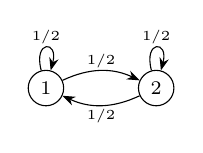
\begin{tikzpicture}[baseline=-0.6ex]
          \node[agent] (a) at (0,0) {1}; \node[agent] (b) at (1.4,0) {2};
          \draw[edge] (a) to[bend left=25] node[weight, above] {1/2} (b);
          \draw[edge] (b) to[bend left=25] node[weight, below] {1/2} (a);
          \draw[selfloop] (a) to node[weight, above] {1/2} (a);
          \draw[selfloop] (b) to node[weight, above] {1/2} (b);
        \end{tikzpicture}
      & $\left[\begin{smallmatrix} 1/2 & 1/2 \\ 1/2 & 1/2 \end{smallmatrix}\right]$
      & $\{1,\, 0\}$
      & $A$ primitive / $G$ strongly connected and aperiodic
      & consensus \\
    (ii)
      & 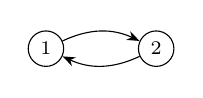
\begin{tikzpicture}[baseline=-0.6ex]
          \node[agent] (a) at (0,0) {1}; \node[agent] (b) at (1.4,0) {2};
          \draw[edge] (a) to[bend left=25] (b);
          \draw[edge] (b) to[bend left=25] (a);
        \end{tikzpicture}
      & $\left[\begin{smallmatrix} 0 & 1 \\ 1 & 0 \end{smallmatrix}\right]$
      & $\{1,\, -1\}$
      & $A$ irreducible, not primitive / $G$ strongly connected and periodic
      & no convergence \\
    (iii)
      & 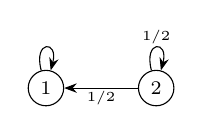
\begin{tikzpicture}[baseline=-0.6ex]
          \node[agent] (a) at (0,0) {1}; \node[agent] (b) at (1.4,0) {2};
          \draw[edge] (b) to node[weight, below] {1/2} (a);
          \draw[selfloop] (a) to (a);
          \draw[selfloop] (b) to node[weight, above] {1/2} (b);
        \end{tikzpicture}
      & $\left[\begin{smallmatrix} 1 & 0 \\ 1/2 & 1/2 \end{smallmatrix}\right]$
      & $\{1,\, 1/2\}$
      & $1$ simple and strictly dominant, $A$ not primitive / $C(G)$ has a unique sink, which is aperiodic
      & consensus \\
    (iv)
      & 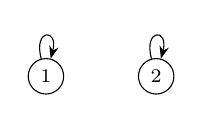
\begin{tikzpicture}[baseline=-0.6ex]
          \node[agent] (a) at (0,0) {1}; \node[agent] (b) at (1.4,0) {2};
          \draw[selfloop] (a) to (a);
          \draw[selfloop] (b) to (b);
        \end{tikzpicture}
      & $\left[\begin{smallmatrix} 1 & 0 \\ 0 & 1 \end{smallmatrix}\right]$
      & $\{1,\, 1\}$
      & $1$ semi-simple but not simple, strictly dominant / $C(G)$ has at least two sinks, all aperiodic
      & disagreement \\
    (v)
      & 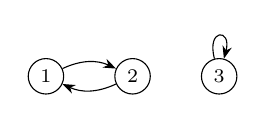
\begin{tikzpicture}[baseline=-0.6ex]
          \node[agent] (a) at (0,0) {1}; \node[agent] (b) at (1.1,0) {2};
          \node[agent] (c) at (2.2,0) {3};
          \draw[edge] (a) to[bend left=25] (b);
          \draw[edge] (b) to[bend left=25] (a);
          \draw[selfloop] (c) to (c);
        \end{tikzpicture}
      & $\left[\begin{smallmatrix} 0 & 1 & 0 \\ 1 & 0 & 0 \\ 0 & 0 & 1 \end{smallmatrix}\right]$
      & $\{1,\, 1,\, -1\}$
      & $1$ not strictly dominant / $G$ not strongly connected, at least one sink of $C(G)$ is periodic
      & no convergence \\
    \bottomrule
  \end{tabular}

  \vspace{1mm}
  {\tiny Cases (i)--(iv) and the examples follow [1]; the properties of case (v), left
  blank in the slides, follow from [5].}
  % REVISED (2026-11-16, buttons: the Rosetta stone has its own slide). Was:
  % \detailbuttons{\ret{m-fdg-model}}
  \detailbuttons{\ret{m-fdg-rosetta}}
\end{frame}

\begin{frame}[label=bk-stubborn]{Stubborn agents in the FDG}
  \scriptsize
  \begin{block}{Definition 2.5 (Stubbornness) [5]}
    An agent is said to be \emph{stubborn} if its opinion remains unchanged independent of
    the others' opinions.
  \end{block}
  If the opinions obey the FDG model, then agent $i$ is stubborn, $x_i(k) \equiv x_i(0)$,
  if and only if $a_{ii} = 1$ [5] (and hence $a_{ij} = 0$ for all $j \neq i$, since $A$ is
  row-stochastic). In the digraph, a stubborn agent is a strongly connected component made
  of a single node, which is a sink of $C(G)$ and is aperiodic because of its self-loop.
  If every agent is influenced by the stubborn agent $i$, then $i$ is the only globally
  reachable node, and Theorem~2.2 gives $w = e_i$.
  \begin{block}{Corollary 2.6 [5]}
    Let the group have $s \geq 1$ stubborn agents, influencing all other individuals (i.e.\
    every other node of $G$ is connected by a walk to the set of stubborn nodes). Then the
    FDG model (1) is convergent.
  \end{block}
  \begin{block}{Remark 2.7 (More than one stubborn agent)}
    If two or more agents are stubborn, each of them is a sink of $C(G)$ made of a single,
    aperiodic node. If every other agent is influenced, directly or through intermediaries,
    by at least one stubborn agent, these are the only sinks, and the group converges
    (Corollary~2.6) to a disagreement (Theorem~2.4): every stubborn agent keeps its own
    initial opinion, and every other agent converges to a convex combination of the
    opinions of the stubborn agents it is influenced by. Since there is no single consensus
    value, the social power is no longer defined.
  \end{block}
  % REVISED (2026-11-11, buttons: m-fdg-power is replaced by m-fdg-disagreement). Was:
  % \detailbuttons{\ret{m-fdg-power}}
  % REVISED (2026-11-16, buttons: also reached from m-bridge). Was:
  % \detailbuttons{\ret{m-fdg-disagreement}}
  % REVISED (2026-11-16, buttons: the bridge is now "Two stubborn agents"). Was:
  % \detailbuttons{\ret[Back to disagreement]{m-fdg-disagreement}\ \ret[Back to the bridge]{m-bridge}}
  \detailbuttons{\ret[Back to disagreement]{m-fdg-disagreement}\ \ret[Back to two stubborn agents]{m-bridge}}
\end{frame}

\begin{frame}[label=bk-spectra]{Spectra of $A(t)$}
  \small
  \begin{itemize}
    \item $t = 0$. Directed cycle: permutation matrix with $A^6 = I$, so its spectrum is the
          set of the sixth roots of unity. Bidirectional ring: circulant, with eigenvalues
          $\cos(2\pi k/6)$, $k = 0, \dots, 5$, i.e.\
          $\{1, \frac12, \frac12, -\frac12, -\frac12, -1\}$. Some eigenvalues different from
          $1$ lie on the unit circle: they cause the oscillations.
    \item $t > 0$: all the eigenvalues different from $1$ lie strictly inside the unit
          disk, and the group converges. For $t = 1/2$ the largest of their moduli,
          computed numerically, is $\approx 0.92$ on the directed cycle, where the
          characteristic polynomial of $A(1/2)$ is
          $\lambda^5(\lambda - \tfrac12) - \tfrac12$, and $\approx 0.90$ on the
          bidirectional ring.
    \item $t = 1$, directed cycle, agent~$1$ listed first: $A(1)$ is block lower
          triangular,
          \[ A(1) = \begin{bmatrix} 1 & 0 \\ b & N \end{bmatrix}, \qquad
             b = (0, 0, 0, 0, 1)^\top, \]
          where $b$ records that agent~$6$ listens to agent~$1$ and the block $N$ of agents
          $2, \dots, 6$ is strictly upper triangular, since agent~$i$ copies agent~$i+1$.
          Hence $N^5 = 0$, the eigenvalue $0$ has multiplicity $5$, and
          $A(1)^5 = \mathbf{1}_6 e_1^\top$: after five steps every agent holds $x_1(0)$.
  \end{itemize}
  \detailbuttons{\ret{m-fdg-conv}}
\end{frame}

\begin{frame}[label=bk-socialpower]{Social power $w(t)$}
  \small
  \begin{itemize}
    \item $0 < t < 1$: strongly connected, every agent globally reachable, so every agent
          has a positive social power (Theorem~2.2(i)). $t = 1$: agent~$1$ is the only
          globally reachable node, $w = e_1$.
    \item In between, $w$ is the left eigenvector of $A(t)$ for the eigenvalue $1$,
          normalized to sum $1$ (condition (A2) of Theorem~2.2). Substituting
          $w = (w_1, b, \dots, b)$ in $w^\top A(t) = w^\top$: in both networks agents
          $2, \dots, 6$ receive the same total weight from the others, and the equations
          reduce to $b = (1-t)\, w_1$. Hence
          \[ w(t) = \frac{1}{1 + 5(1-t)}\,\big(1,\ 1-t,\ 1-t,\ 1-t,\ 1-t,\ 1-t\big)^\top . \]
    % REVISED (2026-11-16, terms: 1/6 is a limit, at t = 0 there is no social power). Was:
    % \item $w_1 = 1/(1 + 5(1-t))$ grows from $1/6$ to $1$; for $t = 1/2$, $w_1 = 2/7$ and
    \item $w_1 = 1/(1 + 5(1-t))$ grows from $1/6$ (limit for $t \to 0$) to $1$; for $t = 1/2$, $w_1 = 2/7$ and
          $w_i = 1/7$ for $i \neq 1$.
    \item Consensus value (Theorem~2.2(ii)), with $x(0) = (0, 0.2, 0.4, 0.6, 0.8, 1)^\top$:
          \[ w(t)^\top x(0) = \frac{3(1-t)}{6 - 5t}, \]
          from the average $0.5$ for $t \to 0$ to $x_1(0) = 0$ for $t = 1$, and $3/7$ for
          $t = 1/2$.
  \end{itemize}
  \detailbuttons{\ret{m-fdg-sp}}
\end{frame}

% ---------------------------------------------------------------------------
% FJ model: theory
% ---------------------------------------------------------------------------

% REMOVED (2026-11-11, terms): Definition 3.1, the decomposition (6)-(7) and Theorem 3.2
% are now on the main slide m-fj-conv. Was:
% \begin{frame}[label=bk-fj-thm]{Theorem 3.2}
%   \scriptsize
%   \begin{block}{Definition 3.1 (P-dependent agents) [5]}
%     Agent $i$ is \emph{P-dependent} if it is prejudiced or influenced by some prejudiced
%     agent $j$, that is, a walk from $i$ to $j$ in the graph $G$ exists. Otherwise, the agent
%     is \emph{P-independent}.
%   \end{block}
%   Agents $1, \dots, r$ P-dependent, $r+1, \dots, n$ P-independent: $W^{21} = 0$,
%   $\Lambda^{22} = I$, and [5]
%   \[
%     x^1(k+1) = \Lambda^{11}\bigl[W^{11} x^1(k) + W^{12} x^2(k)\bigr]
%                + (I - \Lambda^{11})\, u^1 \;\; (6), \qquad
%     x^2(k+1) = W^{22} x^2(k) \;\; (7).
%   \]
%   \begin{block}{Theorem 3.2 [5]}
%     Let the community have $r \geq 1$ P-dependent agents and $n - r \geq 0$ P-independent
%     ones. Then, the subsystem (6) is asymptotically stable, i.e.\ $\Lambda^{11} W^{11}$ is
%     Schur stable $\rho(\Lambda^{11} W^{11}) < 1$. The model (4) is convergent if and only if
%     $r = n$ or (7) is convergent, i.e.\ $W^{22}$ is regular. In this case
%     \[
%       x^1(\infty) = V \begin{bmatrix} u^1 \\ x^2(\infty) \end{bmatrix}, \qquad
%       V \triangleq (I_r - \Lambda^{11} W^{11})^{-1}
%           \begin{bmatrix} I_r - \Lambda^{11} & \Lambda^{11} W^{12} \end{bmatrix}.
%     \]
%     The matrix $V$ is stochastic, i.e.\ the final opinion of any agent is a convex
%     combination of the prejudices and final opinions of P-independent agents.
%   \end{block}
%   \detailbuttons{\go{bk-fj-stab}{Stability}\ \ret{m-fj-conv}}
% \end{frame}

\begin{frame}[label=bk-fj-stab]{Asymptotic stability}
  \scriptsize
  \begin{block}{Corollary 3.3 [5]}
    The Friedkin--Johnsen model (4) is asymptotically stable if and only if all agents are
    P-dependent. Then, $V = (I - \Lambda W)^{-1}(I - \Lambda)$. This holds, in particular,
    if $\Lambda < I_n$ or $\Lambda \neq I_n$ and $G$ is strongly connected ($W$ is
    irreducible).
  \end{block}
  \textbf{With the tools of the course.} Row $i$ of $\Lambda W$ sums to $\lambda_i$: rows of
  agents that are not prejudiced sum to $1$, rows of prejudiced agents to less than $1$, so
  $\Lambda W$ is row-substochastic (Definition~1.13) and Lemma~1.14 applies: every agent that
  is not prejudiced must be influenced, directly or through intermediaries, by a prejudiced
  agent, i.e.\ all agents are P-dependent.

  \medskip
  \textbf{Intuition.} $x(\infty) = Vu$ satisfies $x(\infty) = \Lambda W x(\infty) + (I -
  \Lambda)u$, since $(I - \Lambda W)V = I - \Lambda$. With $e(k) = x(k) - x(\infty)$:
  \[ e(k+1) = \Lambda W\, e(k) \qquad (10), \]
  an autonomous system without $u$: $\Lambda W$ decides whether the opinions converge, $u$
  decides where. Componentwise $e_i(k+1) = \lambda_i \sum_j w_{ij}\, e_j(k)$: a prejudiced
  agent loses a fraction $1 - \lambda_i$ of the deviations, so they vanish only if every
  agent is influenced by a prejudiced agent.
  % REVISED (2026-11-19, notes of 19/11: Corollary 3.3 is now on m-fj-conv3). Was:
  % \detailbuttons{\go{bk-fj-stab2}{Convergence, spectrum}\ \go{bk-prelim3}{Lemma 1.14}\ \ret{m-fj-conv}}
  \detailbuttons{\go{bk-fj-stab2}{Convergence, spectrum}\ \go{bk-prelim3}{Lemma 1.14}\ \ret{m-fj-conv3}}
\end{frame}

\begin{frame}[label=bk-fj-stab2]{Convergence and spectrum}
  \footnotesize
  \begin{block}{Corollary 3.4 [5]}
    The model (4) converges if and only if $\Lambda W$ is regular, i.e.\ the limit
    $\lim_{k \to \infty} (\Lambda W)^k$ exists.
  \end{block}
  \textbf{Theorem 3.2 by $r$.} $r = 0$: not covered, $\Lambda = I$ is the FDG model.
  $0 < r < n$: the P-independent agents follow the FDG model with $W^{22}$, read on the
  sinks of $C^{22}$. $r = n$: no P-independent agents, the model always converges
  (Corollary~3.3).

  \medskip
  Not trivial [5]: a system $x(k+1) = A x(k) + B u$ with a regular matrix $A$ may not
  converge, and may even have unbounded solutions, as for $A = B = I$.

  \medskip
  \textbf{Spectrum.} Listing the P-dependent agents first,
  \[
    \Lambda W = \begin{bmatrix} \Lambda^{11} W^{11} & \Lambda^{11} W^{12} \\ 0 & W^{22}
    \end{bmatrix},
    \qquad
    \operatorname{spec}(\Lambda W) = \operatorname{spec}(\Lambda^{11} W^{11}) \cup
    \operatorname{spec}(W^{22}),
  \]
  and $\rho(\Lambda^{11} W^{11}) < 1$ (Theorem~3.2): the eigenvalues on the unit circle
  can only come from $W^{22}$, i.e.\ from the FDG model of the P-independent agents.
  Asymptotically stable when $r = n$; convergent when the eigenvalue $1$ of $W^{22}$ is
  semi-simple and its other eigenvalues lie inside the unit disk, i.e.\ $W^{22}$ regular.
  % REVISED (2026-11-17, preview: the button "Spectrum" is now on m-fj-conv2). Was:
  % \detailbuttons{\ret[Back to stability]{bk-fj-stab}\ \ret{m-fj-conv}}
  \detailbuttons{\ret[Back to stability]{bk-fj-stab}\ \ret{m-fj-conv2}}
\end{frame}

\begin{frame}[label=bk-fj-consensus]{Consensus in the FJ model}
  \small
  All agents P-dependent: $x_i(\infty) = \sum_{j=1}^{n} v_{ij}\, u_j$, so
  \begin{itemize}
    \item the initial opinions are forgotten: $x(0)$ does not appear in $x(\infty)$;
    \item only the prejudices of prejudiced agents count: if $\lambda_j = 1$, the $j$-th
          column of $I - \Lambda$ is zero, hence so is the $j$-th column of $V$;
    \item every final opinion lies between the smallest and the largest prejudice of the
          prejudiced agents.
  \end{itemize}
  For a given $u$, consensus if $x(\infty) = \gamma\,\mathbf{1}_n$. Since
  $W\mathbf{1}_n = \mathbf{1}_n$, $\gamma\mathbf{1}_n$ is an equilibrium iff
  \[ \gamma\,\mathbf{1}_n = \Lambda W \gamma\,\mathbf{1}_n + (I - \Lambda)\, u
     \iff (I - \Lambda)(\gamma\,\mathbf{1}_n - u) = 0, \]
  i.e.\ $(1 - \lambda_i)(\gamma - u_i) = 0$ for every agent $i$; when all agents are
  P-dependent the equilibrium is unique and equal to $Vu$ (Corollary~3.3).
  \begin{alertblock}{}
    When all agents are P-dependent, the FJ model reaches a consensus if and only if all
    the prejudiced agents have the same prejudice, and the group agrees on it.
  \end{alertblock}
  \detailbuttons{\ret{m-fj-final}}
\end{frame}

\begin{frame}[label=bk-augmented]{The augmented model}
  \small
  Each agent $i$ gets a virtual agent $i'$ with $x_{i'}(k) = u_i$ for all $k$ [5]:
  \[
    \begin{bmatrix} x(k+1) \\ x'(k+1) \end{bmatrix}
    = \underbrace{\begin{bmatrix} \Lambda W & I - \Lambda \\ 0 & I \end{bmatrix}}_{\bar A}
      \begin{bmatrix} x(k) \\ x'(k) \end{bmatrix},
    \qquad x'(0) = u . \qquad (11)
  \]
  Row $i$ of $\bar A$ sums to $\lambda_i + (1 - \lambda_i) = 1$, row $i'$ to $1$: an FDG
  model on $2n$ agents. In the augmented graph a real agent $i$ listens to $j$ with weight
  $\lambda_i w_{ij}$ and to $i'$ with weight $1 - \lambda_i$; $i'$ listens only to itself:
  it is stubborn.
  % REVISED (2026-11-11, terms: sinks of the condensation digraph of the augmented graph;
  % n >= 2, as in the report). Was:
  %   \item Every virtual agent is an aperiodic sink: at least $n$ sinks, so cases (i),
  %         (ii), (iii) never occur.
  \begin{itemize}
    \item Every virtual agent is an aperiodic sink of the condensation digraph of the
          augmented graph: at least $n$ sinks, so for $n \geq 2$ cases (i), (ii), (iii)
          never occur.
    \item \emph{Disagreement} (case (iv)) when all sinks are aperiodic: with all agents
          P-dependent the only sinks are the virtual agents, and every real agent converges
          to a convex combination of the prejudices, i.e.\ (9); otherwise the closed groups
          of P-independent agents are further sinks, all aperiodic iff $W^{22}$ is regular.
    \item \emph{No convergence} (case (v)) when a sink of $C^{22}$ is periodic.
  \end{itemize}
  % REVISED (2026-11-16, buttons: also reached from m-six-sinks). Was:
  % \detailbuttons{\go{bk-augmented2}{Two descriptions}\ \ret{m-fj-final}}
  \detailbuttons{\go{bk-augmented2}{Two descriptions}\ \ret[Back to final opinions]{m-fj-final}\ \ret[Back to six sinks]{m-six-sinks}}
\end{frame}

\begin{frame}[label=bk-augmented2]{Two descriptions, one dynamics}
  \small
  With all agents P-dependent, the FJ model is asymptotically stable (Corollary~3.3),
  while the augmented model (11), row-stochastic, is never asymptotically stable: it
  converges to the disagreement of case (iv), which depends on $x'(0) = u$. $\bar A$ is
  block triangular, so
  \[
    \operatorname{spec}(\bar A) = \operatorname{spec}(\Lambda W) \cup
    \{\underbrace{1, \dots, 1}_{n}\}.
  \]
  \begin{itemize}
    \item The eigenvalues of $\Lambda W$ lie inside the unit disk: the FJ model, which has
          only these, is asymptotically stable.
    \item The augmented model adds the eigenvalue $1$ once for each virtual agent,
          semi-simple by Theorem~2.4 applied to its $n$ aperiodic sinks: the prejudices,
          which in the augmented model are \alert{states}.
    \item In the FJ model $u$ is an \alert{input}: asymptotic stability concerns the
          perturbations of $x(0)$ with $u$ fixed, which die out as in (10); changing $u$
          is a different input, with a different equilibrium $Vu$.
  \end{itemize}
  \detailbuttons{\ret[Back to the augmented model]{bk-augmented}\ \ret{m-fj-final}}
\end{frame}

\begin{frame}[label=bk-centrality]{Influence centrality}
  \small
  Asymptotically stable FJ model with $u = x(0)$ [5]: $x(\infty) = V x(0)$, and
  \[ c = n^{-1} V^\top \mathbf{1}_n, \qquad
     \bar x = \frac{1}{n} \sum_{i=1}^{n} x_i(\infty) = \frac{1}{n} \mathbf{1}_n^\top V x(0)
            = c^\top x(0). \qquad (12) \]
  $c_i$ is the average of the $i$-th column of $V$; $V$ stochastic gives $c \geq 0$ and
  $c^\top \mathbf{1}_n = 1$. For $\Lambda = \alpha I_n$, $\alpha \in [0,1)$: for $\alpha = 0$,
  $V = I$ and $c_0 = n^{-1}\mathbf{1}_n$ [5].
  \begin{block}{Lemma 3.5 [5]}
    Let $W$ be a fully regular matrix and $w$ stand for the vector of French's social power,
    corresponding to the FDG model (1) with $A = W$. Then, $w = \lim_{\alpha \to 1-0}
    c_\alpha$.
  \end{block}
  As $\alpha \to 1$, $V_\alpha = (1 - \alpha)(I - \alpha W)^{-1} \to \mathbf{1}_n w^\top$
  [5]: the final opinions approach the FDG consensus, and $c_\alpha \to w$. The limit
  cannot be replaced by $\alpha = 1$: for $\Lambda = I$ the FJ model is the FDG model, which
  is not asymptotically stable, and $I - W$ is singular since $1 \in \operatorname{spec}(W)$
  (Theorem~1.6), so $V$ is not defined.
  % REVISED (2026-11-17, preview: the button "Lemma 3.5" is now on m-lemma). Was:
  % \detailbuttons{\ret{m-fj-centrality}}
  \detailbuttons{\ret{m-lemma}}
\end{frame}

% ---------------------------------------------------------------------------
% FJ model: examples
% ---------------------------------------------------------------------------

\begin{frame}[label=bk-state-input]{How a perturbation evolves}
  \small
  $x(k)$, $\tilde x(k)$: trajectories of Figures 6 and 7, $\delta(k) = \tilde x(k) - x(k)$.
  \begin{itemize}
    \item FJ: $u$ is the same in the two runs, so $\delta(k+1) = \Lambda W\, \delta(k)$, the
          recursion of the error (10). All agents P-dependent: $\Lambda W$ Schur stable,
          $\delta(k) \to 0$, the two runs reach the same $Vu$.
    \item FDG: $\delta(k+1) = A\,\delta(k)$ and, by Theorem~2.2,
          $\delta(k) \to (w^\top \delta(0))\mathbf{1}_6 = 0.5\,\mathbf{1}_6$, since
          $w = e_1$ and $\delta(0) = 0.5\, e_1$: never forgotten.
  \end{itemize}
  \textbf{Spectra.} $\Lambda W$ and $A(1)$ differ only in the row of agent~$1$: zero in
  $\Lambda W$, $e_1^\top$ in $A(1)$. Listing agent~$1$ first, both are block lower
  triangular, with diagonal entry $0$ or $1$ for agent~$1$ and the same block for agents
  $2, \dots, 6$.
  \begin{itemize}
    \item Ring: the block is $\tfrac12$ times the adjacency matrix of the path graph on
          five nodes, whose spectrum is $\{2\cos(k\pi/6) \mid k = 1, \dots, 5\}$ [4], so the
          block has eigenvalues $\cos(k\pi/6)$:
          $\operatorname{spec}(\Lambda W) = \{0, 0, \pm\tfrac12, \pm\tfrac{\sqrt3}{2}\}$,
          $\operatorname{spec}(A(1)) = \{1, 0, \pm\tfrac12, \pm\tfrac{\sqrt3}{2}\}$.
    \item Cycle: the block is the nilpotent $N$: all eigenvalues $0$, except the eigenvalue
          $1$ of $A(1)$, that of the virtual agent $1'$.
  \end{itemize}
  \detailbuttons{\ret{m-state-input}}
\end{frame}

\begin{frame}[label=bk-rewritings]{From one model to the other}
  \centering
  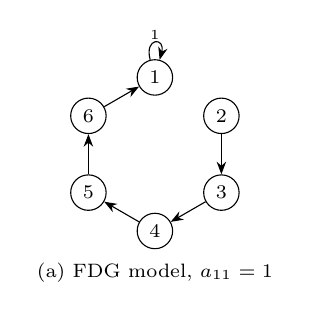
\begin{tikzpicture}[baseline=(c.base), scale=0.75]
    \foreach \i in {1,...,6} {
      \node[agent] (rd\i) at ({90-60*(\i-1)}:1.3) {\i};
    }
    \node (c) at (0,0) {};
    \foreach \i/\j in {2/3,3/4,4/5,5/6,6/1} {
      \draw[edge] (rd\i) -- (rd\j);
    }
    \draw[selfloop] (rd1) to node[weight, above] {$1$} (rd1);
    \node at (0,-2.0) {\scriptsize (a) FDG model, $a_{11} = 1$};
  \end{tikzpicture}
  \hspace{1.5cm}
  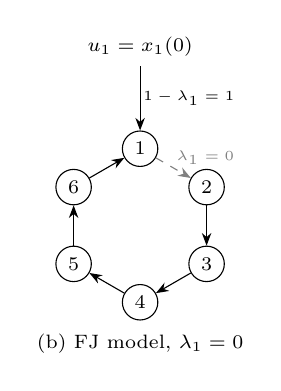
\begin{tikzpicture}[baseline=(c.base), scale=0.75]
    \foreach \i in {1,...,6} {
      \node[agent] (rf\i) at ({90-60*(\i-1)}:1.3) {\i};
    }
    \node (c) at (0,0) {};
    \foreach \i/\j in {2/3,3/4,4/5,5/6,6/1} {
      \draw[edge] (rf\i) -- (rf\j);
    }
    \draw[edge, dashed, gray] (rf1) -- node[weight, above right] {$\lambda_1 = 0$} (rf2);
    \draw[edge] (0,2.7) node[above, font=\scriptsize] {$u_1 = x_1(0)$}
      -- node[weight, right] {$1-\lambda_1 = 1$} (rf1);
    \node at (0,-2.0) {\scriptsize (b) FJ model, $\lambda_1 = 0$};
  \end{tikzpicture}

  {\scriptsize Figure 5: the rewriting of [5] on the directed cycle with $t = 1$.}

  \vspace{2mm}
  \raggedright
  \footnotesize
  \begin{itemize}
    \item $\lambda_i = 0$ and $u_i = x_i(0)$ for every stubborn agent, $\lambda_i = 1$ (and
          any $u_i$) for the others: the two models produce the same trajectories.
    \item The row of $W$ of a stubborn agent plays no role, since it is multiplied by
          $\lambda_i = 0$. The stubborn agent turns from a state into an input; its opinion
          appears twice, as $x_i(0)$ and as $u_i = x_i(0)$.
  \end{itemize}
  \detailbuttons{\go{bk-rewritings2}{Second rewriting}\ \ret{m-state-input}}
\end{frame}

\begin{frame}[label=bk-rewritings2]{The stubborn agent as a prejudice}
  \centering
  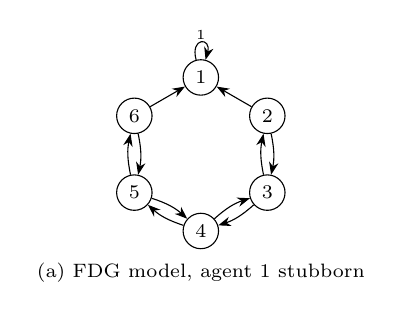
\begin{tikzpicture}[baseline=(c.base), scale=0.75]
    \foreach \i in {1,...,6} {
      \node[agent] (sa\i) at ({90-60*(\i-1)}:1.3) {\i};
    }
    \node (c) at (0,0) {};
    \foreach \i/\j in {2/3,3/4,4/5,5/6} {
      \draw[edge] (sa\i) to[bend left=12] (sa\j);
      \draw[edge] (sa\j) to[bend left=12] (sa\i);
    }
    \draw[edge] (sa2) -- (sa1);
    \draw[edge] (sa6) -- (sa1);
    \draw[selfloop] (sa1) to node[weight, above] {$1$} (sa1);
    \node at (0,-2.0) {\scriptsize (a) FDG model, agent~$1$ stubborn};
  \end{tikzpicture}
  \hspace{1.5cm}
  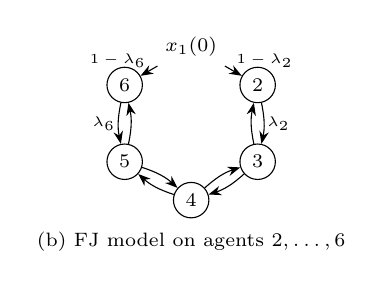
\begin{tikzpicture}[baseline=(c.base), scale=0.75]
    \foreach \i in {2,...,6} {
      \node[agent] (sb\i) at ({90-60*(\i-1)}:1.3) {\i};
    }
    \node (c) at (0,0) {};
    \node[font=\scriptsize] (su) at (90:1.3) {$x_1(0)$};
    \foreach \i/\j in {3/4,4/5} {
      \draw[edge] (sb\i) to[bend left=12] (sb\j);
      \draw[edge] (sb\j) to[bend left=12] (sb\i);
    }
    \draw[edge] (sb2) to[bend left=12] node[weight, right] {$\lambda_2$} (sb3);
    \draw[edge] (sb3) to[bend left=12] (sb2);
    \draw[edge] (sb6) to[bend right=12] node[weight, left] {$\lambda_6$} (sb5);
    \draw[edge] (sb5) to[bend right=12] (sb6);
    \draw[edge] (su) -- node[weight, above right] {$1-\lambda_2$} (sb2);
    \draw[edge] (su) -- node[weight, above left] {$1-\lambda_6$} (sb6);
    \node at (0,-2.0) {\scriptsize (b) FJ model on agents $2, \dots, 6$};
  \end{tikzpicture}

  {\scriptsize Figure 8: bidirectional ring with $t = 1$; every edge between agents has
  weight $1/2$.}

  \vspace{2mm}
  \raggedright
  \footnotesize
  \begin{itemize}
    \item An agent $i$ that listens to the stubborn agent~$1$ updates as
          $x_i(k+1) = \sum_{j \neq 1} a_{ij}\, x_j(k) + a_{i1}\, x_1(0)$, which is (5) with
          $\lambda_i = 1 - a_{i1}$, $w_{ij} = a_{ij}/\lambda_i$, $u_i = x_1(0)$.
    \item On the ring: $\lambda_2 = \lambda_6 = 1/2$, $u_2 = u_6 = x_1(0)$,
          $\lambda_3 = \lambda_4 = \lambda_5 = 1$: the augmented graph read backwards. The
          stubborn opinion appears only once, as a prejudice.
  \end{itemize}
  % REVISED (2026-11-16, buttons: also reached from m-bridge). Was:
  % \detailbuttons{\ret[Back to the first rewriting]{bk-rewritings}\ \ret{m-state-input}}
  % REVISED (2026-11-16, buttons: Figure 8 is now reached from m-back-question). Was:
  % \detailbuttons{\ret[Back to the first rewriting]{bk-rewritings}\ \ret[Back to state or input]{m-state-input}\ \ret[Back to the bridge]{m-bridge}}
  \detailbuttons{\ret[Back to the first rewriting]{bk-rewritings}\ \ret[Back to state or input]{m-state-input}\ \ret[Back to the question]{m-back-question}}
\end{frame}

\begin{frame}[label=bk-one-prej]{A single prejudice}
  \small
  On the directed cycle:
  \[
    {\setlength{\arraycolsep}{3pt}
    \Lambda W = \begin{bmatrix}
       0&\frac12&0&0&0&0\\ 0&0&1&0&0&0\\ 0&0&0&1&0&0\\ 0&0&0&0&1&0\\ 0&0&0&0&0&1\\ 1&0&0&0&0&0
    \end{bmatrix},
    \qquad
    A(\tfrac12) = \begin{bmatrix}
       \frac12&\frac12&0&0&0&0\\ 0&0&1&0&0&0\\ 0&0&0&1&0&0\\ 0&0&0&0&1&0\\ 0&0&0&0&0&1\\ 1&0&0&0&0&0
    \end{bmatrix}}
  \]
  The weight $1/2$ taken off the agent it listens to goes, in $A(1/2)$, to the diagonal
  (current opinion), and in the FJ model out of the matrix, to the input
  $(1 - \lambda_1)u_1$; the first row of $\Lambda W$ sums to $1/2$.
  \begin{itemize}
    \item Strongly connected: all agents P-dependent, asymptotically stable
          (Corollary~3.3, case $\Lambda \neq I_n$, $W$ irreducible).
    \item Column $j$ of $V$ is zero when $\lambda_j = 1$ and $V$ is stochastic:
          $V = \mathbf{1}_6 e_1^\top$, $x(\infty) = u_1\mathbf{1}_6 = 0$, $c = e_1$.
    \item Augmented graph: $2', \dots, 6'$ have weight $0$, nobody listens to them; the
          rest has the single sink $1'$, so it reaches a consensus with social power
          $e_{1'}$: with $u = x(0)$, the group converges to $x_1(0)$.
  \end{itemize}
  \detailbuttons{\ret{m-one-prej}}
\end{frame}

\begin{frame}[label=bk-all-prej]{Every agent prejudiced}
  \small
  On the directed cycle:
  \[
    {\setlength{\arraycolsep}{3pt}
    A = 0.2\, I + 0.8\, W = \begin{bmatrix}
       0.2&0.8&0&0&0&0\\ 0&0.2&0.8&0&0&0\\ 0&0&0.2&0.8&0&0\\ 0&0&0&0.2&0.8&0\\
       0&0&0&0&0.2&0.8\\ 0.8&0&0&0&0&0.2
    \end{bmatrix},
    \qquad
    \Lambda W = 0.8\, W = \begin{bmatrix}
       0&0.8&0&0&0&0\\ 0&0&0.8&0&0&0\\ 0&0&0&0.8&0&0\\ 0&0&0&0&0.8&0\\
       0&0&0&0&0&0.8\\ 0.8&0&0&0&0&0
    \end{bmatrix}}
  \]
  \begin{itemize}
    \item FDG: $A$ row- and column-stochastic with positive diagonal, primitive
          (Corollary~1.12): consensus on the average $0.5$ (Corollary~2.3).
    \item FJ: $\Lambda < I_6$, asymptotically stable (Corollary~3.3),
          $x(\infty) = Vu$ with $V = 0.2\,(I - 0.8\,W)^{-1}$, stochastic, with all entries
          positive since $W$ is irreducible: every prejudice enters every final opinion,
          with weights that change from row to row; the prejudices differ, so no consensus.
    \item Augmented graph: six stubborn virtual agents with different opinions, as in
          Remark~2.7.
  \end{itemize}
  \detailbuttons{\ret{m-all-prej}}
\end{frame}

\begin{frame}[label=bk-aux]{Auxiliary network: blocks}
  \scriptsize
  Order $\sigma = (4, 5 \mid 1, 2, 3, 6)$, $P = [\, e_4\ e_5\ e_1\ e_2\ e_3\ e_6 \,]^\top$; for
  $W_{\mathrm{a}}$:
  \[
    \tilde W_{\mathrm{a}} = P\, W_{\mathrm{a}} P^\top =
    \left[\begin{array}{cc|cccc}
      0 & 1 & 0 & 0 & 0 & 0\\
      0 & 0 & 0 & 0 & 0 & 1\\ \hline
      0 & 0 & 0 & 1 & 0 & 0\\
      0 & 0 & \tfrac12 & 0 & \tfrac12 & 0\\
      0 & 0 & 1 & 0 & 0 & 0\\
      0 & 0 & 1 & 0 & 0 & 0
    \end{array}\right]
    = \begin{bmatrix} W^{11} & W^{12} \\ 0 & W^{22} \end{bmatrix},
    \qquad
    \tilde\Lambda = \mathrm{diag}(1,\, 0.5 \mid 1,\, 1,\, 1,\, 1).
  \]
  The lower-left block is zero: no P-independent agent listens to a P-dependent one. With
  $\Lambda^{11} = \mathrm{diag}(1, 0.5)$, Theorem~3.2 gives
  \[
    V = (I_2 - \Lambda^{11} W^{11})^{-1}\big[\, I_2 - \Lambda^{11},\ \Lambda^{11} W^{12} \,\big]
      = \left[\begin{array}{cc|cccc}
          0 & 0.5 & 0 & 0 & 0 & 0.5\\ 0 & 0.5 & 0 & 0 & 0 & 0.5
        \end{array}\right],
    \quad x_4(\infty) = x_5(\infty) = 0.5\, u_5 + 0.5\, x_6(\infty).
  \]
  Social power of the closed group $\{1, 2, 3\}$, from its block of $W^{22}$
  (Theorem~2.2): $w_1 = \tfrac12 w_2 + w_3$, $w_2 = w_1$, $w_3 = \tfrac12 w_2$, sum $1$
  $\Rightarrow$ $(0.4, 0.4, 0.2)$.
  \begin{itemize}
    \item (c): consensus $0.4 \cdot 0 + 0.4 \cdot 0.5 + 0.2 \cdot 1 = 0.4$, agent~$6$ follows
          agent~$1$, agents $4, 5$ at $0.5 \cdot 0.9 + 0.5 \cdot 0.4 = 0.65$.
    \item (d): $x_2(0) = 1$, consensus $0.4 \cdot 1 + 0.2 \cdot 1 = 0.6$, agents $4, 5$ at
          $0.5 \cdot 0.9 + 0.5 \cdot 0.6 = 0.75$. In the augmented model the closed group
          adds a seventh eigenvalue $1$.
  \end{itemize}
  \detailbuttons{\go{bk-aux-table}{Summary}\ \ret{m-aux}}
\end{frame}

\begin{frame}[label=bk-aux-table]{Auxiliary network: Table 2}
  \centering
  \scriptsize
  \renewcommand{\arraystretch}{1.25}
  \begin{tabular}{@{}c c >{\raggedright\arraybackslash}p{2.3cm} c >{\raggedright\arraybackslash}p{4.2cm} >{\raggedright\arraybackslash}p{3.6cm}@{}}
    \toprule
    Panel & $W$ & Prejudiced agent & P-dependent & Outcome & What it shows \\
    \midrule
    (a) & $W_{\mathrm{p}}$ & $2$, inside the closed group & all ($r = n$)
        & asymptotically stable (Corollary~3.3),
          $x(\infty) = u_2 \mathbf{1}_6 = 0.5\, \mathbf{1}_6$
        & the periodic cycle plays no role \\
    \midrule
    (b) & $W_{\mathrm{p}}$ & $5$, outside the closed group & $4, 5$ ($r = 2$)
        & $W^{22}$ not regular: not convergent (Theorem~3.2)
        & aperiodicity is needed again, for the P-independent agents \\
    \midrule
    (c) & $W_{\mathrm{a}}$ & $5$, outside the closed group & $4, 5$ ($r = 2$)
        & $W^{22}$ regular: convergent (Theorem~3.2), not asymptotically stable; agents
          $1,2,3,6$ at $0.4$, agents $4,5$ at $0.65$
        & convergence without asymptotic stability (Corollary~3.4) \\
    \midrule
    (d) & $W_{\mathrm{a}}$ & as (c), $x_2(0) = 1$, $u$ unchanged & $4, 5$ ($r = 2$)
        & as (c), but agents $1,2,3,6$ at $0.6$, agents $4,5$ at $0.75$
        & the limit depends on the initial opinions of the P-independent agents \\
    \bottomrule
  \end{tabular}
  \detailbuttons{\ret[Back to blocks and $V$]{bk-aux}\ \ret{m-aux}}
\end{frame}

\begin{frame}[label=bk-lemma-numbers]{The numbers of Figure 13}
  \small
  \begin{itemize}
    \item $W = A(1/2)$: strongly connected with a self-loop, primitive (Corollary~1.12),
          hence fully regular, as Lemma~3.5 requires. $\Lambda = \alpha I$,
          $\alpha \in [0, 0.995]$ (the lemma takes $\alpha < 1$), $u = x(0)$.
    \item $\alpha = 0$: $V = I$, so $c_0 = \frac16 \mathbf{1}_6$ (dotted line $1/6$).
    \item $\alpha \to 1$: $c_\alpha \to w$, the social power of the FDG model with
          $A = A(1/2)$: $w_1 = 2/7$, $w_2 = \dots = w_6 = 1/7$ (dashed lines), from
          $w(t)$ at $t = 1/2$.
    \item On the directed cycle $c_2$ first goes below $w_2$: its computed minimum is about
          $0.137$, at $\alpha \approx 0.65$.
    \item $c_\alpha$ exists on every network: $\rho(\alpha W) = \alpha < 1$ for every
          stochastic $W$, also where $w$ does not exist.
  \end{itemize}
  \detailbuttons{\ret{m-lemma}}
\end{frame}

% ADDED (2026-11-22, notes of 22/11: V_alpha and c_alpha in closed form on the two networks,
% from the formulas of the report, Section 3.1.4 and (12); computed by us, checked with sympy).
\begin{frame}[label=bk-lemma-V,t]{$V_\alpha$ and $c_\alpha$ in closed form}
  \only<1>{%
  \footnotesize
  $x(\infty) = V_\alpha\, x(0)$, $V_\alpha = (1-\alpha)(I - \alpha W)^{-1}$, $W = A(\frac12)$;
  $c_\alpha = \frac16 V_\alpha^\top \mathbf{1}_6$ (12): $c_j(\alpha)$ is the mean of column $j$
  of $V_\alpha$.
  \par\medskip
  \textbf{Directed cycle}, with $D(\alpha) = 2 + \alpha + \alpha^2 + \alpha^3 + \alpha^4 + \alpha^5$:
  {\setlength{\arraycolsep}{4pt}\renewcommand{\arraystretch}{1.1}%
  \[ V_\alpha = \frac{1}{D(\alpha)} \begin{bmatrix}
       2 & \alpha & \alpha^2 & \alpha^3 & \alpha^4 & \alpha^5 \\
       2\alpha^5 & 2-\alpha & \alpha(2-\alpha) & \alpha^2(2-\alpha) & \alpha^3(2-\alpha) & \alpha^4(2-\alpha) \\
       2\alpha^4 & \alpha^5 & 2-\alpha & \alpha(2-\alpha) & \alpha^2(2-\alpha) & \alpha^3(2-\alpha) \\
       2\alpha^3 & \alpha^4 & \alpha^5 & 2-\alpha & \alpha(2-\alpha) & \alpha^2(2-\alpha) \\
       2\alpha^2 & \alpha^3 & \alpha^4 & \alpha^5 & 2-\alpha & \alpha(2-\alpha) \\
       2\alpha & \alpha^2 & \alpha^3 & \alpha^4 & \alpha^5 & 2-\alpha
     \end{bmatrix} \]}
  \[ c_1(\alpha) = \frac13 - \frac{1}{3D(\alpha)}, \qquad
     c_j(\alpha) = \frac16 - \frac{\alpha^{j-1}}{6D(\alpha)}, \quad j = 2, \dots, 6. \]
  $\alpha = 0$: $D = 2$, every $c_j = \frac16$. $\alpha \to 1$: $D \to 7$, $c_1 \to \frac27$,
  $c_j \to \frac17$. Agents $2, \dots, 6$: the same form, only the power $\alpha^{j-1}$
  changes.}%
  \only<2>{%
  \footnotesize
  $x(\infty) = V_\alpha\, x(0)$, $V_\alpha = (1-\alpha)(I - \alpha W)^{-1}$, $W = A(\frac12)$;
  $c_\alpha = \frac16 V_\alpha^\top \mathbf{1}_6$ (12): $c_j(\alpha)$ is the mean of column $j$
  of $V_\alpha$.
  \par\medskip
  \textbf{Bidirectional ring}, with $E(\alpha) = 8 + 4\alpha - 4\alpha^2 - \alpha^3$ and
  $p = 4 - \alpha^2$:
  {\setlength{\arraycolsep}{5pt}\renewcommand{\arraystretch}{1.1}%
  \[ V_\alpha = \frac{1}{p\,E(\alpha)} \begin{bmatrix}
       2p(4-3\alpha^2) & \alpha p q & \alpha^2 p & \alpha^3 p & \alpha^2 p & \alpha p q \\
       2\alpha p q & f & \alpha q r & \alpha^2 (2-\alpha) p & \alpha^3 h & \alpha^2(4-\alpha^3) \\
       2\alpha^2 p & \alpha q r & g & \alpha p s & \alpha^2 r & \alpha^3 h \\
       2\alpha^3 p & \alpha^2 (2-\alpha) p & \alpha p s & p k & \alpha p s & \alpha^2 (2-\alpha) p \\
       2\alpha^2 p & \alpha^3 h & \alpha^2 r & \alpha p s & g & \alpha q r \\
       2\alpha p q & \alpha^2(4-\alpha^3) & \alpha^3 h & \alpha^2 (2-\alpha) p & \alpha q r & f
     \end{bmatrix} \]}
  {\scriptsize $q = 2-\alpha^2$, $r = 8-4\alpha-\alpha^2$, $s = 4-2\alpha-\alpha^2$,
  $h = 6-2\alpha-\alpha^2$, $k = 8-4\alpha-4\alpha^2+\alpha^3$,
  $f = 32-16\alpha-28\alpha^2+12\alpha^3+4\alpha^4-\alpha^5$,
  $g = 32-16\alpha-24\alpha^2+8\alpha^3+3\alpha^4$.\par}
  \[ c_1 = \frac{(1+\alpha)(4-\alpha^2)}{3E}, \quad
     c_2 = c_6 = \frac{4+\alpha-2\alpha^2}{3E}, \quad
     c_3 = c_5 = \frac{(1+\alpha)(8-4\alpha-\alpha^2)}{6E}, \quad
     c_4 = \frac{(2+\alpha)(2-\alpha^2)}{3E}. \]
  $\alpha = 0$: $E = 8$, every $c_j = \frac16$. $\alpha \to 1$: $E \to 7$, $c_1 \to \frac27$,
  $c_j \to \frac17$. Symmetric with respect to agent~$1$.}%
  \detailbuttons{\ret{m-lemma}}
\end{frame}

% ---------------------------------------------------------------------------
% Conclusions and references
% ---------------------------------------------------------------------------

\begin{frame}[label=bk-table]{Comparison (Table 3)}
  \centering
  \scriptsize
  \renewcommand{\arraystretch}{0.95}
  \begin{tabular}{@{}>{\raggedright\arraybackslash}p{2.4cm}
                  >{\raggedright\arraybackslash}p{5.7cm}
                  >{\raggedright\arraybackslash}p{6.0cm}@{}}
    \toprule
    & FDG model (1) & FJ model (4) \\
    \midrule
    Resistance to the others
      & self-weight $a_{ii}$: inertia, a weight on the current opinion
      & attachment $1 - \lambda_i$ to the prejudice $u_i$: an anchor to a fixed value \\
    Stubborn agent (Def.~2.5)
      & $a_{ii} = 1$: a condition on the matrix only
      & $\lambda_i = 0$ and $u_i = x_i(0)$: a condition on the matrix and on the input \\
    Opinion of a stubborn agent & a state & an input \\
    Convergence
      & Table~1: sinks of $C(G)$ and their aperiodicity
      & all agents P-dependent (Corollary~3.3), or $W^{22}$ regular (Theorem~3.2) \\
    Asymptotic stability
      & never: the eigenvalue $1$ lies on the unit circle (Theorem~1.6)
      & if and only if all agents are P-dependent, i.e.\ $\rho(\Lambda W) < 1$
        (Corollary~3.3) \\
    Final opinions
      & consensus $(w^\top x(0))\mathbf{1}_n$ (Theorem~2.2), or disagreement with at least
        two aperiodic sinks (Theorem~2.4)
      & if all agents are P-dependent, $x(\infty) = Vu$ (9): convex combinations of the
        prejudices, independent of $x(0)$ \\
    Strongly connected network
      & consensus or no convergence, never disagreement
      & disagreement whenever the prejudices that count differ \\
    Aperiodicity & always needed & needed only for the P-independent agents \\
    Measure of power
      & social power $w$ (2): requires a consensus
      & influence centrality $c$ (12): requires $\rho(\Lambda W) < 1$ and $u = x(0)$ \\
    From one model to the other
      & with stubborn agents, an FJ model with $\lambda_i = 0$, $u_i = x_i(0)$ for the
        stubborn agents [5], or, removing them, an FJ model in which their opinions are
        prejudices (Figure~8)
      & an FDG model on the augmented graph (11), with $n$ virtual stubborn agents \\
    \bottomrule
  \end{tabular}
  \detailbuttons{\ret{m-table}}
\end{frame}

\begin{frame}[label=bk-refs]{References}
  \small
  \begin{enumerate}
    \item[{[1]}] Giacomo Baggio. DT averaging systems. Lecture slides, Network Dynamical
          Systems, University of Padova, 2025.
    \item[{[2]}] Giacomo Baggio. Elements of Graph Theory. Lecture slides, Network
          Dynamical Systems, University of Padova, 2025.
    \item[{[3]}] Giacomo Baggio. Elements of Matrix Theory. Lecture slides, Network
          Dynamical Systems, University of Padova, 2025.
    \item[{[4]}] Francesco Bullo. Lectures on Network Systems. Kindle Direct Publishing,
          1.7 edition, 2024. With contributions by J.\ Cort\'es, F.\ D\"orfler, and
          S.\ Mart\'inez.
    \item[{[5]}] Anton V.\ Proskurnikov and Roberto Tempo. A tutorial on modeling and
          analysis of dynamic social networks. Part I. Annual Reviews in Control,
          43:65--79, 2017.
  \end{enumerate}
\end{frame}

% ADDED (2026-11-23, notes of 23/11): slides moved here from the main line, to save time.

\begin{frame}[label=m-prelim]{Preliminaries}
  \footnotesize
  \begin{columns}[T]
    \column{0.49\textwidth}
      \textbf{Graphs} [1, 2]
      \begin{itemize}
        \item Edge $(i,j)$, $i \to j$, weight $a_{ij} > 0$: agent $i$ is influenced by
              agent $j$; $A = [a_{ij}]$ the (weighted) adjacency matrix.
        \item \alert{Strongly connected}: a directed walk from any node to any other
              node. \alert{Globally reachable} node: reached from any other node.
        \item A strongly connected digraph is \alert{periodic} if an integer $k > 1$
              divides the length of every simple cycle; otherwise \alert{aperiodic}.
              A self-loop makes it aperiodic.
        \item \alert{Condensation digraph} $C(G)$: each strongly connected component
              collapsed into a single node. \alert{Sink}: a node with no outgoing edges,
              i.e.\ a group influenced only by itself.
      \end{itemize}
    \column{0.49\textwidth}
      \textbf{Matrices} [2, 3]
      \begin{itemize}
        \item \alert{Row-stochastic}: $A \geq 0$, $A\mathbf{1}_n = \mathbf{1}_n$;
              \alert{doubly-stochastic}: also $A^\top\mathbf{1}_n = \mathbf{1}_n$.
        \item \alert{Semi-convergent}: $\lim_{k \to +\infty} A^k$ exists (finite);
              \alert{convergent} (Schur stable): the limit is $0_{n \times n}$, iff
              $\rho(A) < 1$.
        \item Eigenvalue $1$ \alert{simple} (algebraic = geometric multiplicity $= 1$),
              \alert{semi-simple} (algebraic = geometric multiplicity),
              \alert{strictly dominant} (all other eigenvalues have modulus $< 1$).
        \item \alert{Irreducible} ($n \geq 2$) iff $G$ is strongly connected;
              \alert{primitive}, i.e.\ $A^k > 0$ for some $k$, iff $G$ is strongly
              connected and aperiodic.
      \end{itemize}
  \end{columns}
  \detailbuttons{\go{bk-graphs}{Graphs}\ \go{bk-prelim}{Matrices}\ \ret[Back to the FDG model]{m-fdg-model}}
\end{frame}

\begin{frame}[label=m-fdg-rosetta]{Which outcome: the Rosetta stone}
  \centering
  \footnotesize
  The outcome can be read on the spectrum of $A$, on the matrix $A$, or on the digraph
  $G$; the Rosetta stone of the course links the three.

  \vspace{2mm}
  \renewcommand{\arraystretch}{1.25}
  \begin{tabular}{@{}c >{\raggedright\arraybackslash}p{4.4cm}
                    >{\raggedright\arraybackslash}p{5.2cm} l@{}}
    \toprule
    Case & Property of $A$ & Property of $G$ & Outcome \\
    \midrule
    (i)   & $A$ primitive
          & $G$ strongly connected and aperiodic
          & consensus \\
    (ii)  & $A$ irreducible, not primitive
          & $G$ strongly connected and periodic
          & no convergence \\
    (iii) & $1$ simple and strictly dominant, $A$ not primitive
          & $C(G)$ has a unique sink, which is aperiodic
          & consensus \\
    (iv)  & $1$ semi-simple but not simple, strictly dominant
          & $C(G)$ has at least two sinks, all aperiodic
          & disagreement \\
    (v)   & $1$ not strictly dominant
          & $G$ not strongly connected, at least one sink of $C(G)$ is periodic
          & no convergence \\
    \bottomrule
  \end{tabular}

  \vspace{1mm}
  {\scriptsize Rosetta stone [1]: Table~1 without the examples. The properties of case
  (v), left blank in [1], follow from [5].}

  % REVISED (2026-11-19, layout: the translation at full width, Corollary 1.12 narrower, so
  % that it stays clear of the four buttons). Was: \vspace{2mm}, minipage 0.80.
  \vspace{1.5mm}
  \raggedright
  % ADDED (2026-11-19, notes of 19/11): where the translation between A and G comes from,
  % as in the report (Section 2.1.4).
  The translation between $A$ and $G$ comes from the characterizations of irreducible and
  primitive matrices (Theorem~1.11) in cases (i)--(ii), and from Theorems~2.2 and~2.4 in
  cases (iii)--(iv).

  \smallskip
  \begin{minipage}{0.62\textwidth}
    \textbf{Corollary 1.12} [2]: if $G$, of order $n \geq 2$, has at least one self-loop
    and is strongly connected, then $A$ is primitive.
    % REVISED (2026-11-19, notes of 19/11: the slide now follows consensus and disagreement;
    % the focus of the work is on m-fdg-consensus). Was:
    % \smallskip
    % Focus of this work: \alert{consensus}, the case in which the weight of each agent can
    % be measured (next slide); disagreement in one slide after it.
  \end{minipage}
  % REVISED (2026-11-19, buttons: Theorem 1.11 is named on the slide). Was:
  % \detailbuttons{\go{bk-graphs}{Graphs}\ \go{bk-prelim}{Matrices}\ \go{bk-rosetta}{Table 1}}
  \detailbuttons{\go{bk-graphs}{Graphs}\ \go{bk-prelim}{Matrices}\ \go{bk-prelim2}{Theorem 1.11}\ \go{bk-rosetta}{Table 1}\ \ret[Back to disagreement]{m-fdg-disagreement}}
\end{frame}

\begin{frame}[label=m-fj-matrices]{FJ on the same networks: $W$ and $\Lambda$}
  \footnotesize
  % REVISED (2026-11-22, notes of 22/11: W is the FDG matrix A(0), strongly connected and
  % periodic). Was:
  % $W = A(0)$: the networks of «Two networks, one agent», without self-loops. Prejudices
  % $u = x(0) = (0, 0.2, \dots, 1)^\top$, as in the original FJ model.
  $W = A(0)$: the networks of «Two networks, one agent», without self-loops, strongly
  connected and periodic. With $\Lambda = I$ the FJ model is the FDG model with $A(0)$: the
  opinions do not converge. Prejudices $u = x(0) = (0, 0.2, \dots, 1)^\top$, as in the
  original FJ model.

  {\setlength{\arraycolsep}{3.5pt}\renewcommand{\arraystretch}{0.8}%
  \begin{columns}[c]
    \column{0.44\textwidth}
      \centering
      Directed cycle: \
      $W = \begin{bmatrix}
        0&1&0&0&0&0\\ 0&0&1&0&0&0\\ 0&0&0&1&0&0\\ 0&0&0&0&1&0\\ 0&0&0&0&0&1\\ 1&0&0&0&0&0
      \end{bmatrix}$
    \column{0.52\textwidth}
      \centering
      Bidirectional ring: \
      $W = \dfrac12 \begin{bmatrix}
        0&1&0&0&0&1\\ 1&0&1&0&0&0\\ 0&1&0&1&0&0\\ 0&0&1&0&1&0\\ 0&0&0&1&0&1\\ 1&0&0&0&1&0
      \end{bmatrix}$
  \end{columns}}

  \smallskip
  \scriptsize
  \renewcommand{\arraystretch}{1.1}
  \begin{tabular}{@{}lllll@{}}
    \toprule
    & \textbf{FJ}: $\Lambda$ & $I - \Lambda$ & $\Lambda W$ & \textbf{FDG}: $A$ \\
    \midrule
    Agent~$1$ stubborn & $\operatorname{diag}(0, 1, \dots, 1)$
      & $\operatorname{diag}(1, 0, \dots, 0)$ & $W$ with row~$1$ times $0$ & $A(1)$ \\
    Agent~$1$ with weight $t$ & $\operatorname{diag}(1-t, 1, \dots, 1)$
      & $\operatorname{diag}(t, 0, \dots, 0)$ & $W$ with row~$1$ times $1-t$ & $A(t)$ \\
    Every agent with weight $0.2$ & $0.8\,I$ & $0.2\,I$ & $0.8\,W$ & $0.2\,I + 0.8\,W$ \\
    \bottomrule
  \end{tabular}

  \smallskip
  % REVISED (2026-11-23): smaller, for the return buttons. Was: \footnotesize
  \scriptsize
  \begin{itemize}
    \setlength{\itemsep}{1pt}
    \item $\Lambda W$ multiplies row~$i$ of $W$ by $\lambda_i$: its entries are the weights
          on the edges of the FJ graphs (b), (d), (f), (h).
    \item In the three cases $A$ and $\Lambda W$ have the same weights on the others. The rest of row~$i$,
          $1 - \lambda_i$, is on the current opinion $x_i(k)$ in the FDG model (diagonal of
          $A$), on the prejudice $u_i$ in the FJ model (out of the matrix):
          $A = \Lambda W + (I - \Lambda)$.
    % ADDED (2026-11-22, notes of 22/11: one prejudice is enough).
    \item \alert{One prejudiced agent is enough}: $G$ is strongly connected, so every agent
          has a path to agent~$1$ and is P-dependent; by Corollary~3.3 the FJ model is
          asymptotically stable. No aperiodicity is needed. In the FDG model the same
          change of one agent, a self-weight $t > 0$, gives consensus by making $G$
          aperiodic.
  \end{itemize}
  \detailbuttons{\go{m-fj-matrices-all}{Next}\ \ret[Back to the networks]{m-fj-graphs}}
\end{frame}

\begin{frame}[label=m-fj-matrices-all]{Every agent with weight $0.2$: the matrices}
  \footnotesize
  $\Lambda = 0.8\,I$, $I - \Lambda = 0.2\,I$, $u = x(0)$: every agent gives weight $0.2$ to
  its current opinion in the FDG model, to its prejudice in the FJ model.
  % ADDED (2026-11-22, notes of 22/11: why this case; report, Section 3.2.2).
  \alert{Why this case:} with one prejudice the FJ model still reaches a consensus,
  $u_1\mathbf{1}_6$; with a different prejudice for every agent it disagrees on the same
  strongly connected network on which the FDG model can only agree. This is the main
  difference between the two models.

  \smallskip

  \smallskip
  {\setlength{\arraycolsep}{3pt}\renewcommand{\arraystretch}{0.85}\scriptsize
  \begin{tabular}{@{}r@{\ \ }c@{\qquad}c@{}}
    & \textbf{FDG}: $A = 0.2\,I + 0.8\,W$ & \textbf{FJ}: $\Lambda W = 0.8\,W$ \\ \noalign{\vskip 3pt}
    directed cycle &
    $\begin{bmatrix}
      0.2&0.8&0&0&0&0\\ 0&0.2&0.8&0&0&0\\ 0&0&0.2&0.8&0&0\\ 0&0&0&0.2&0.8&0\\
      0&0&0&0&0.2&0.8\\ 0.8&0&0&0&0&0.2
    \end{bmatrix}$ &
    $\begin{bmatrix}
      0&0.8&0&0&0&0\\ 0&0&0.8&0&0&0\\ 0&0&0&0.8&0&0\\ 0&0&0&0&0.8&0\\
      0&0&0&0&0&0.8\\ 0.8&0&0&0&0&0
    \end{bmatrix}$ \\ \noalign{\vskip 6pt}
    bidirectional ring &
    $\begin{bmatrix}
      0.2&0.4&0&0&0&0.4\\ 0.4&0.2&0.4&0&0&0\\ 0&0.4&0.2&0.4&0&0\\ 0&0&0.4&0.2&0.4&0\\
      0&0&0&0.4&0.2&0.4\\ 0.4&0&0&0&0.4&0.2
    \end{bmatrix}$ &
    $\begin{bmatrix}
      0&0.4&0&0&0&0.4\\ 0.4&0&0.4&0&0&0\\ 0&0.4&0&0.4&0&0\\ 0&0&0.4&0&0.4&0\\
      0&0&0&0.4&0&0.4\\ 0.4&0&0&0&0.4&0
    \end{bmatrix}$
  \end{tabular}\par}

  % REVISED (2026-11-23): smaller, for the return buttons. Was: \footnotesize
  \scriptsize
  \begin{itemize}
    \setlength{\itemsep}{1pt}
    \item $A$: row- and column-stochastic, i.e.\ doubly-stochastic, with a positive diagonal:
          $G$ strongly connected and aperiodic, so consensus, with $w = \frac16\mathbf{1}_6$:
          the average $0.5$ of $x(0)$.
    \item $\Lambda W$: every row sums to $0.8$ (row-substochastic); every agent is
          prejudiced, so all P-dependent: asymptotically stable, $x(\infty) = Vu$ (9).
          The final opinions are closer to each other than the initial ones, but not
          equal: the prejudices differ, so no consensus.
  \end{itemize}
  \detailbuttons{\go{m-fj-networks}{Next}\ \ret[Back to the networks]{m-fj-graphs}}
\end{frame}

\begin{frame}[label=m-fj-networks]{FDG and FJ: the updates}
  \footnotesize
  Every cell is an update equation, with the weight of each opinion written out. In (5)
  the weight of $x_j(k)$ in the update of agent~$i$ is $\lambda_i w_{ij}$, the entry
  $(i,j)$ of $\Lambda W$.

  \smallskip
  \scriptsize
  \renewcommand{\arraystretch}{1.3}
  \begin{tabular}{@{}lll@{}}
    \toprule
    & \textbf{FDG}: self-weight $a_{ii}$ on the current opinion $x_i(k)$
    & \textbf{FJ}: attachment $1 - \lambda_i$ to the prejudice $u_i$ \\
    \midrule
    \multicolumn{3}{@{}l}{\textbf{Agent~$1$ stubborn}: $a_{11} = 1$, $\lambda_1 = 0$
      (Figure~6)} \\
    both & $x_1(k+1) = x_1(k)$ & $x_1(k+1) = u_1 = x_1(0)$ \\
    \midrule
    \multicolumn{3}{@{}l}{\textbf{Agent~$1$ with weight $t$}: $a_{11} = t$,
      $1 - \lambda_1 = t$ (graphs (a), (b), (e), (f); Figure~9: $t = \frac12$)} \\
    cycle & $x_1(k+1) = t\,x_1(k) + (1-t)\,x_2(k)$
      & $x_1(k+1) = (1-t)\,x_2(k) + t\,u_1$ \\
    ring & $x_1(k+1) = t\,x_1(k) + \frac{1-t}{2}\,x_2(k) + \frac{1-t}{2}\,x_6(k)$
      & $x_1(k+1) = \frac{1-t}{2}\,x_2(k) + \frac{1-t}{2}\,x_6(k) + t\,u_1$ \\
    \midrule
    \multicolumn{3}{@{}l}{\textbf{Every agent with weight $0.2$}: $A = 0.2\,I + 0.8\,W$,
      $\Lambda = 0.8\,I$ (graphs (c), (d), (g), (h); Figure~10)} \\
    cycle & $x_i(k+1) = 0.2\,x_i(k) + 0.8\,x_{i+1}(k)$
      & $x_i(k+1) = 0.8\,x_{i+1}(k) + 0.2\,u_i$ \\
    ring & $x_i(k+1) = 0.2\,x_i(k) + 0.4\,x_{i-1}(k) + 0.4\,x_{i+1}(k)$
      & $x_i(k+1) = 0.4\,x_{i-1}(k) + 0.4\,x_{i+1}(k) + 0.2\,u_i$ \\
    \bottomrule
  \end{tabular}

  \smallskip
  \footnotesize In the first two cases the other agents are as in $A(0)$ in both models
  ($\lambda_i = 1$).
  \socially{The same weight on a different object: the current opinion, which still moves
  towards the others, or the prejudice, which never moves.}
  \detailbuttons{\ret[Back to the networks]{m-fj-graphs}}
\end{frame}

\begin{frame}[label=m-six-sinks,t]{Six prejudices, six sinks}
  % [t]: the augmented graph does not move between the three steps
  \compactblocks
  \begin{columns}[T]
    \column{0.36\textwidth}
      \centering
      \begin{tikzpicture}[scale=0.7]
        \fill[red_unipd!10] (0,0) circle (1.85);
        \foreach \i in {1,...,6} {
          \pgfmathsetmacro{\ang}{90-60*(\i-1)}
          \node[agent, fill=white] (g\i) at (\ang:1.3) {\i};
          \node[agent, dashed, fill=white, minimum size=5mm] (v\i) at (\ang:2.6) {\i$'$};
        }
        \foreach \i/\j in {1/2,3/4,4/5,5/6,6/1} {
          \draw[edge] (g\i) -- (g\j);
        }
        \draw[edge] (g2) -- node[weight, left] {$0.8$} (g3);
        \foreach \i in {2,...,6} {
          \draw[edge] (g\i) -- (v\i);
        }
        \draw[edge] (g1) -- node[weight, left] {$0.2$} (v1);
        \foreach \i in {2,...,6} {
          \pgfmathsetmacro{\ang}{90-60*(\i-1)}
          \pgfmathsetmacro{\angout}{\ang+28}
          \pgfmathsetmacro{\angin}{\ang-28}
          \draw[edge] (v\i) to[out=\angout, in=\angin, looseness=5, min distance=4mm]
            (v\i);
        }
        \draw[edge] (v1) to[out=118, in=62, looseness=5, min distance=4mm]
          node[weight, right] {$1$} (v1);
        \node at (0,-3.85) {\scriptsize (a) augmented graph of network (d)};
      \end{tikzpicture}
    \column{0.62\textwidth}
      \footnotesize
      \only<1>{%
        {\centering
          \begin{tikzpicture}[scale=0.62]
            \node[circle, fill=red_unipd!10, draw=red_unipd, inner sep=0pt,
                  minimum size=1.15cm, font=\scriptsize] (R) at (0,0) {$\{1,\dots,6\}$};
            \foreach \i in {1,...,6} {
              \pgfmathsetmacro{\ang}{90-60*(\i-1)}
              \node[agent, dashed, minimum size=5mm] (w\i) at (\ang:1.85) {\i$'$};
              \draw[edge] (R) -- (w\i);
            }
            \node[anchor=west, font=\scriptsize] at (2.7,0)
              {(b) condensation digraph: six sinks};
          \end{tikzpicture}\par}
        \smallskip
        Network (d) ($\Lambda = 0.8I$, Figure~10) as an FDG model on $12$ agents (11):
        each prejudice $u_i$ becomes the virtual agent $i'$, stubborn at $u_i$; agent $i$
        gives $0.8$ to the other real agents and $0.2$ to $i'$.

        \smallskip
        Real agents: one strongly connected component (shaded), not a sink. Virtual
        agents: six sinks, aperiodic because of their self-loops.

        \smallskip
        Theorem~2.4 with $n_s = 6$: \alert{case (iv)}, as in Remark~2.7. The same on the
        bidirectional ring.}%
      \only<2>{%
        \begin{itemize}
          \item $x(\infty) = Vu$, $V = 0.2\,(I - 0.8W)^{-1}$ with all entries positive:
                every final opinion is a convex combination of all six prejudices.
          \item Figure~9: six sinks too, but only $1'$ is listened to; without the other
                five, a single sink and a consensus.
        \end{itemize}
        \begin{alertblock}{The FDG disagreement, not forgotten}
          \footnotesize One stubborn agent: consensus (Figure~2, $t = 1$). Two:
          disagreement (Two stubborn agents; Back to the question). Six virtual ones, all
          listened to: here, an FDG model with the disagreement of Theorem~2.4.
        \end{alertblock}}%
      \only<3>{%
        \textbf{Twelve trajectories.} Figure~10 shows only the six real agents; in the
        augmented model the six virtual agents stay at $u_i = x_i(0)$. Every real agent
        starts on the line of its virtual agent and leaves it as soon as the opinions it
        listens to (weight $0.8$) average to a different value: at once on the directed
        cycle; on the ring, agents $2, \dots, 5$ later, when the change of agents $1$ and
        $6$ reaches them. The weight $0.2$ on its virtual agent keeps pulling it back, and
        it settles at $x(\infty) = Vu$, never on its own prejudice. In the FDG model the
        same $0.2$ is on the current opinion: the agent follows the group to the
        consensus.}
  \end{columns}
  \detailbuttons{\go{bk-augmented}{Augmented}\ \ret[Back to every agent prejudiced]{m-all-prej}}
\end{frame}


\end{document}
